\chapter{Top Physics}
\label{chapter:topanalysis}
\section{Introduction}

\begin{figure}
  \centering
  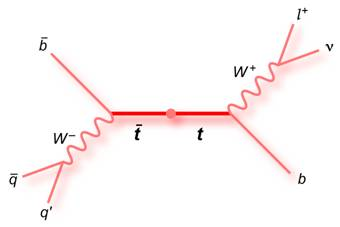
\includegraphics[width=0.5\textwidth]{TopAnalysis/figures/TopFeynmann.jpg}
  \caption[Semileptonic $t\bar{t}$ decay]{Semileptonic $t\bar{t}$ decay}
  \label{fig:topfeynmann}
\end{figure}

Here we give details of an analysis proposed for measuring the top quark forward-backward asymmetry, A$_{FB}^t$, at CLIC during the 1.4 TeV stage. 

As described in Chapter \ref{theory}, A$_{FB}^t$ is sensitive to the electroweak form factors of the $ttX, X=Z,\gamma$ vertex. By measuring A$_{FB}^t$ and the $t\bar{t}$ cross section at multiple energies and with different beam polarizations, it is possible to extract values for many of these form factors and use them as a probe for testing the \ac{SM}. The measurement is well motivated by the existing result for the b quark forward-backward asymmetry observed at \ac{LEP}\cite{ABBIENDI200229}, which is currently the largest deviation from the \ac{SM} within electroweak fits. Due to the limited energy at \ac{LEP} (which is still the highest energy e$^+$e$^-$ collider to have existed,) an analogous measurement of the asymmetry for tops has has yet to be performed at a lepton collider. 

\begin{table}[b]
  \centering
  \begin{tabular}{l |c}
    \toprule
    Decay Mode     & Branching Fraction (\%) \\
    \midrule
    Fully Hadronic, $tt\rightarrow WbWb\rightarrow qqbqqb$ & 45.3  \\
    \midrule
    Semileptonic, $tt\rightarrow WbWb\rightarrow qqbl\nu b$ & 43.8 \\
    \midrule
    Fully Leptonic, $tt\rightarrow WbWb\rightarrow l\nu bl\nu b$ & 10.6 \\
    \midrule
    $tt\rightarrow Other$ & 0.4 \\
    \bottomrule
  \end{tabular}
  \caption[Top Pair Decay Modes]{Top Pair Decay Modes\cite{Patrignani:2016xqp}.}
  \label{table:topdecaymodes}
\end{table}

A$_{FB}$ is defined as:

\begin{equation}
A_{FB}^t=\frac{N_F-N_B}{N_F+N_B},
\end{equation}
where $N_{F}$ and $N_{B}$ are the number of t quarks produced in the forward and backward directions, which are defined to be the regions corresponding to cos$\theta >$($<$)0 respectively, where $\theta$ is the angle of the particles 3-momentum relative to the z-axis.

\begin{figure}[]
  \centering
  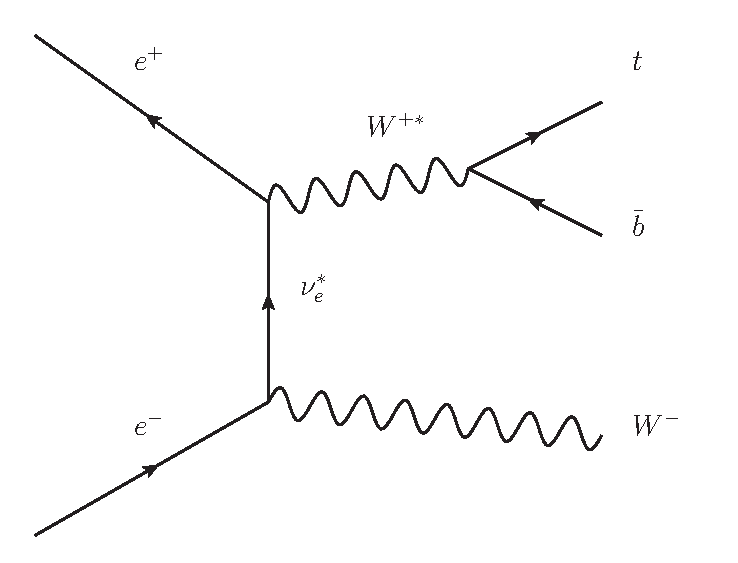
\includegraphics[width=0.5\textwidth]{TopAnalysis/figures/SingleTop}
  \caption[Dominant single top production mode]{Dominant single top production mode capable of mimicking the signal process}
  \label{fig:singletop}
\end{figure}


As tops decay almost exclusively to a W and b (99.8\% of decays) they are typically described in terms of the resulting decay modes of the Ws. The dominant decay modes are described in \reftab{table:topdecaymodes}. Here we will look at measuring $A_{FB}^{t}$ using the semileptonic $t\bar{t}$ decay channel (see \reffig{fig:topfeynmann}) in which one of the W's decays to a lepton and neutrino and the other W decays to a a pair of quarks. This decay mode is ideal for determining $A_{FB}^{t}$ as the lepton from the leptonically decaying top provides the ability to charge tag the top while the hadronic decay allows an accurate measurement of the production angle of the top. Due to the sensitivity of $A_{FB}^{t}$ to polarization states, the measurement will be done for two different electron beam polarizations, -80\% and +80\%, assuming an even split of luminosity between the two configurations. The dominant signal and background processes examined by this analysis, as well as their cross sections and internal \ac{CLIC} production ID numbers for each polarization are shown in \reftabs{table:topsamplesnegpol} and \ref{table:topsamplespospol}. All samples are simulated using the CLIC\_ILD\_CDR detector model. The samples also include an overlay of $\gamma\gamma\rightarrow$ hadron events from beamsstrahlung based on a 30~ns time window around the generated physics events. Because these are inclusive six-fermion final state samples that include contributions from both signal (including $t\bar{t}$) and background amplitudes, before they can be used for this analysis the $e^+e^-\rightarrow qqqql\nu$ samples must be filtered to enhance the signal process. This is done by inspecting all three-fermion combinations of $qqq$ and $ql\nu$ and retaining only those in which the resulting triplets of particles both have masses within 5$\times\Gamma_t$ of $m_t$, where within the generator $m_t$ and $\Gamma_t$ are 174 GeV and 1.4 GeV respectively. In the case that two tops could not be simultaneously identified, the event is described as either single top or non top depending on whether any single combination of $qqq$ or $ql\nu$ is within the correct mass window. The dominant backgrounds are expected to be from alternative $t\bar{t}$ decays (fully hadronic decay modes and semileptonic decays containing taus) and from single top events (see \reffig{fig:singletop}) which will have similar topologies as they can both contain a hadronically decaying top.

\begin{table}
  \centering
  \begin{tabular}{l | r | r |r}
    \toprule
    Process     & Cross Section(fb) & Production ID & Events Used ($\times$10$^{3}$) \\
    \midrule
    $e^+e^-\rightarrow qqqql\nu$ & 142.3 & 6589,6592,6634,6637 & 3860 \\
    \midrule
    $e^+e^-\rightarrow qqqqqq$ & 116.4 & 6595, 6598, 6601, 6604,  & 310 \\
     &  & 6610, 6607, 6613, 6616,  &  \\
     &  &  6619, 6622  &  \\
    \midrule
    $e^+e^-\rightarrow qql\nu l\nu$ & 44.1 & 6586, 6625, 6628, 6631 & 100 \\
    \midrule
    $e^+e^-\rightarrow qqqq$ & 2304 & 8254 & 1,590 \\
    \midrule
    $e^+e^-\rightarrow qql\nu$ & 6975 & 7477 & 3,520 \\
    \midrule
    $e^+e^-\rightarrow qqll$ & 2681 & 8244 & 1,190 \\
    \midrule
    $e^+e^-\rightarrow qq\nu\nu$ & 1395 & 8271 & 1,120 \\
    \midrule
    $e^+e^-\rightarrow qq$ & 4843 & 8283 & 2,400 \\
    \bottomrule
  \end{tabular}
  \caption{Samples used in the -80\% electron beam polarization study.}
  \label{table:topsamplesnegpol}
\end{table}

\begin{table}
  \centering
  \begin{tabular}{l | r | r |r}
    \toprule
    Process     & Cross Section(fb) & Production ID & Events Used (10$^{3}$) \\
    \midrule
    $e^+e^-\rightarrow qqqql\nu$ & 53.5 & 6646, 6697, 6691, 6694 & 160 \\
    \midrule
    $e^+e^-\rightarrow qqqqqq$ & 44.9 & 6652, 6655, 6658, 6661, & 198 \\
     &  & 6664, 6667, 6670, 6673, &  \\
     &  & 6676, 6679 &  \\
    \midrule
    $e^+e^-\rightarrow qql\nu l\nu$ & 15.3  & 6643, 6682, 6685, 6688 & 15.3 \\
    \midrule
    $e^+e^-\rightarrow qqqq$ & 347 & 8257 & 500 \\
    \midrule
    $e^+e^-\rightarrow qql\nu$ & 1640 & 7480 & 1,000 \\
    \midrule
    $e^+e^-\rightarrow qqll$ & 2530 & 8241 & 1,000 \\
    \midrule
    $e^+e^-\rightarrow qq\nu\nu$ & 180 & 8274 & 200 \\
    \midrule
    $e^+e^-\rightarrow qq$ & 3170 & 8286 & 1,500 \\
    \bottomrule
  \end{tabular}
  \caption{Samples used in the +80\% electron beam polarization study.}
  \label{table:topsamplespospol}
\end{table}


The results presented here are included in a paper summarizing the top physics potential at \ac{CLIC}\cite{TopPaperDraft}. Within the paper, an alternative version of this analysis is also performed in which an alternate reconstruction method and event selection are implemented. The results of both analysis have been found to yield consistent results for the expected precision on $A_{FB}^{t}$.


\section{Event Reconstruction}
Reconstruction of signal events is performed using ILCSOFT v01-17-10 and consists of three main stages. The first stage is to identify isolated leptons arising from the leptonically decaying top. These leptons are then removed and the remaining PFOs are resolved into two large radius ``fat jets''. The two fat jets must then be associated with either the b jet produced by the leptonically decaying top or with the combination of three jets arising from the hadronically decaying top. A kinematic fitter is used to reconstruct the neutrino and any \ac{ISR}/\ac{BS} photons present in the event. Throughout the analysis only tight selected PFOs have been considered in the reconstruction (PFOs reconstructed with a timing cut of $\sim$2~ns placed on clusters in the detector\cite{cdrvol2}) so as to reduce beam backgrounds.

\subsection{Lepton Finding}
\label{sec:lepfinding}
Lepton finding is the first stage of reconstruction performed in each event. Due to the fact the measurement of $A_{FB}^{t}$ is entirely reliant on using the lepton charge to distinguish between tops and antitops, it is essential that a high efficiency and purity are achieved and that there is no angular dependence on the performance. For this analysis lepton finding is done in two steps. Firstly, lepton candidates with energy $>$ 10~GeV are identified using the particle ID provided by the Pandora Particle Flow Algorithm \cite{Thomson200925}. Only muons and electrons are examined due to the fact tau leptons require different reconstruction techniques to identify and are typically reconstructed with significantly lower efficiency. This first stage removes $>$ 90\% of fake candidates with negligible impact on efficiency. The second stage of selection is to examine how isolated each of the candidates are. This is evaluated by resolving all PFOs in the event into five jets, then for each lepton candidate measuring the energy of the candidate ($E_{Candidate}$) relative to that of the jet ($E_{Jet}$) with which it was associated. For this process the inclusive ee kt algorithm was chosen for the jet finding to ensure that all lepton candidates are always placed within a jet. The lepton candidate found to have the highest ratio of $E_{Candidate}/E_{Jet}$ is then declared to be the isolated lepton arising from the leptonically decaying top. In the case that no lepton is selected by the first step, the restrictions on the particle ID and energy are relaxed and the lepton is selected purely based on which PFO is the most isolated according to step two. This method ensures that there is always exactly one lepton selected per event. The net efficiency with which this method selects a candidate with the correct charge is found to be 93\% for electrons and 96\% for muons.

\begin{figure}
  \centering
  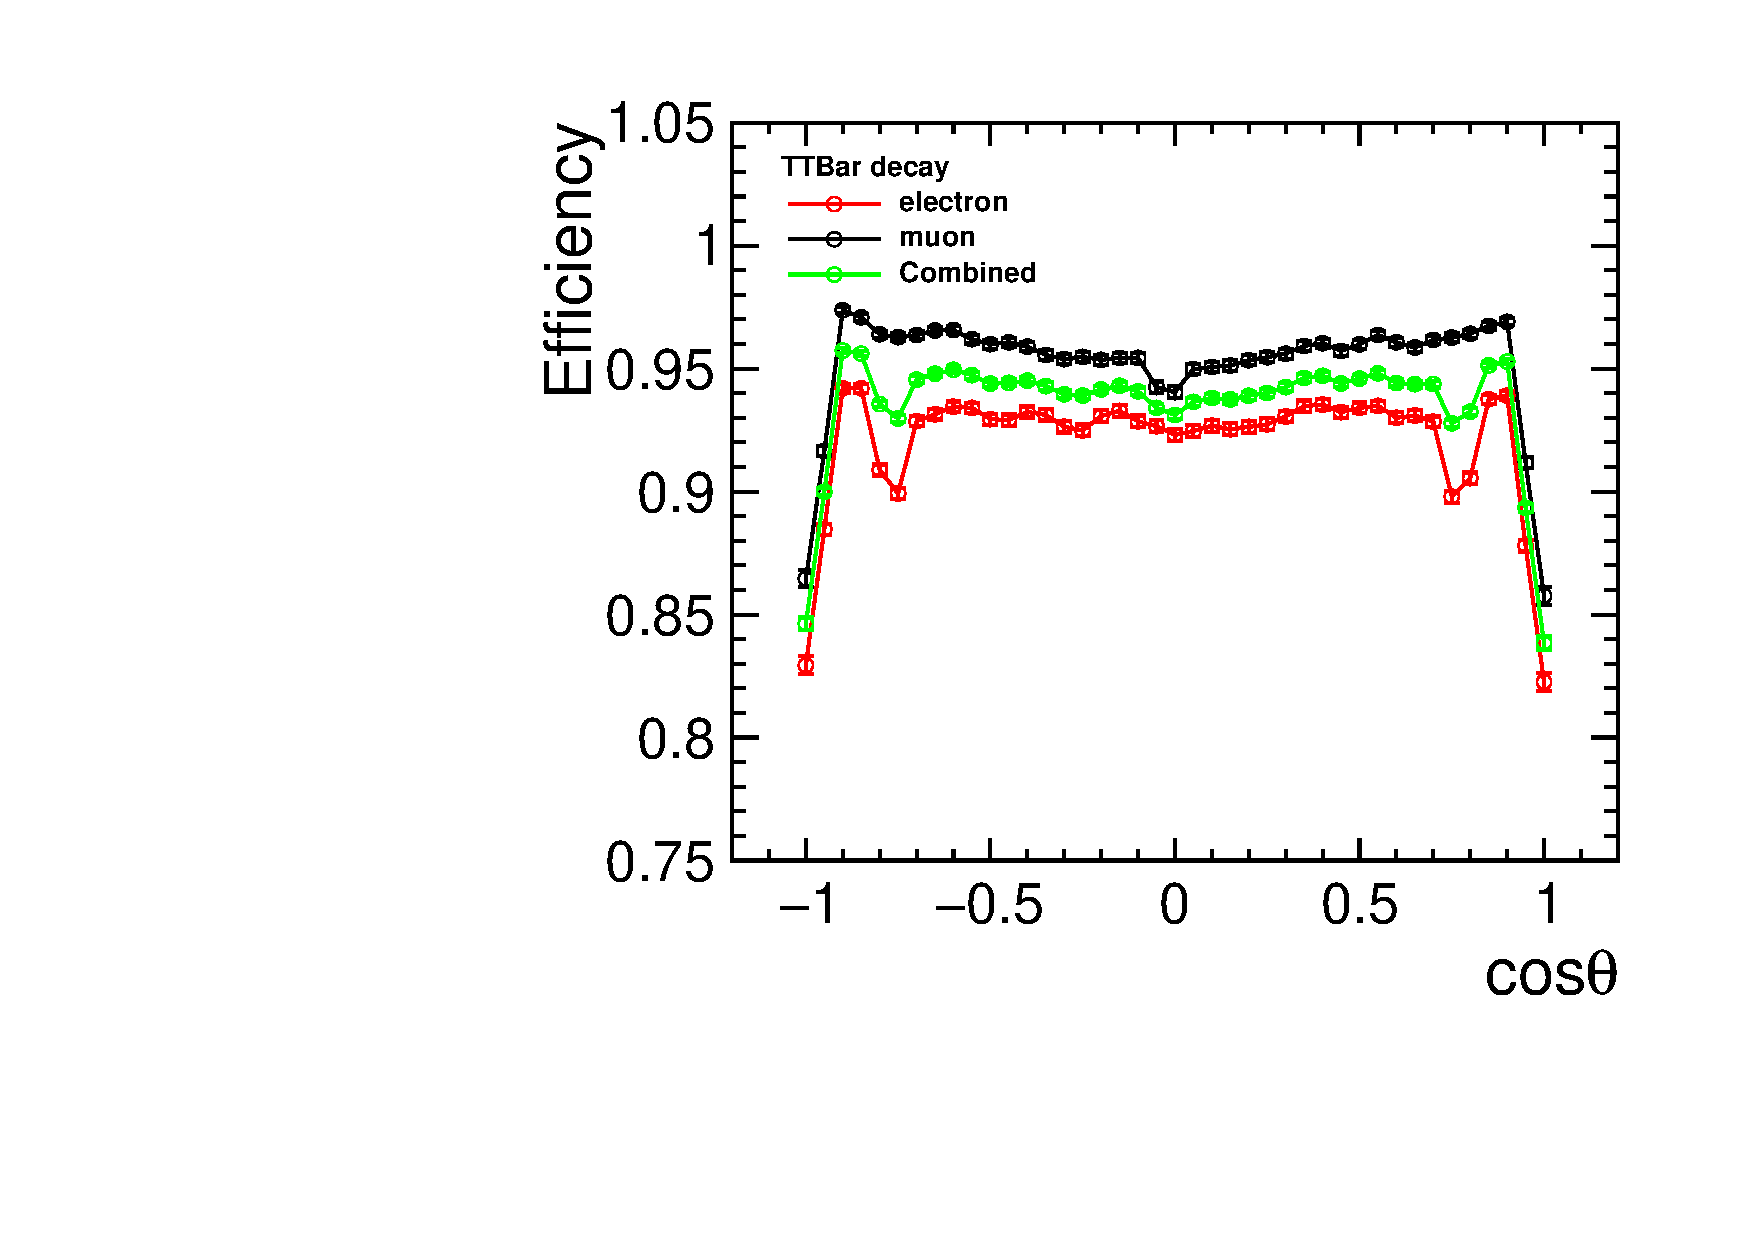
\includegraphics[width=0.7\textwidth]{TopAnalysis/figures/NetEfficiencys.pdf}
  \caption[Efficiency for identifying leptons with the correct charge as a function of angle.]{Efficiency for identifying leptons with the correct charge as a function of angle.}
  \label{fig:netefficiency}
\end{figure}


As well as understanding the net efficiency for finding leptons it is also important to examine the angular dependence of the efficiency to ensure there is no bias that could effect the measurement of $A_{FB}^{t}$. \reffig{fig:netefficiency} shows how the efficiency varies with angle. The efficiency is seen to rapidly decline for $|\cos\theta| > 0.9$ due to the detector acceptance. A decrease in efficiency is also seen for electrons at angles corresponding to the transition point between the ECAL barrel and endcaps. This effect is not seen for muons as they are also reconstructed using the muon detectors placed at a larger radius. Overall the efficiency is seen to be consistently worse for electrons than muons. This is to be expected as muons produce easily recognizable signatures in the detector due to the fact they typically penetrate through the tracker, ECAL, HCAL and muon systems whereas electrons only leave deposits in the tracker and ECAL. In the case that tracks are lost during reconstruction or are wrongly associated to other PFOs it is then possible for photons to be labeled incorrectly as electrons and vice versa leading to a higher fake rate for electrons.

As well as checking the angular dependence of the charge tagging efficiency it is also key to examine the charge dependence of the lepton finding to make sure there is no preference for identifying particles over antiparticles. The angular dependence of the charge tagging efficiency for particles vs antiparticles is shown in \reffig{fig:chargeEfficiencies}. An asymmetry in the performance is observed for both electrons and muons.

\begin{figure}
  \centering
  \begin{subfigure}{.5\textwidth}
    \centering
    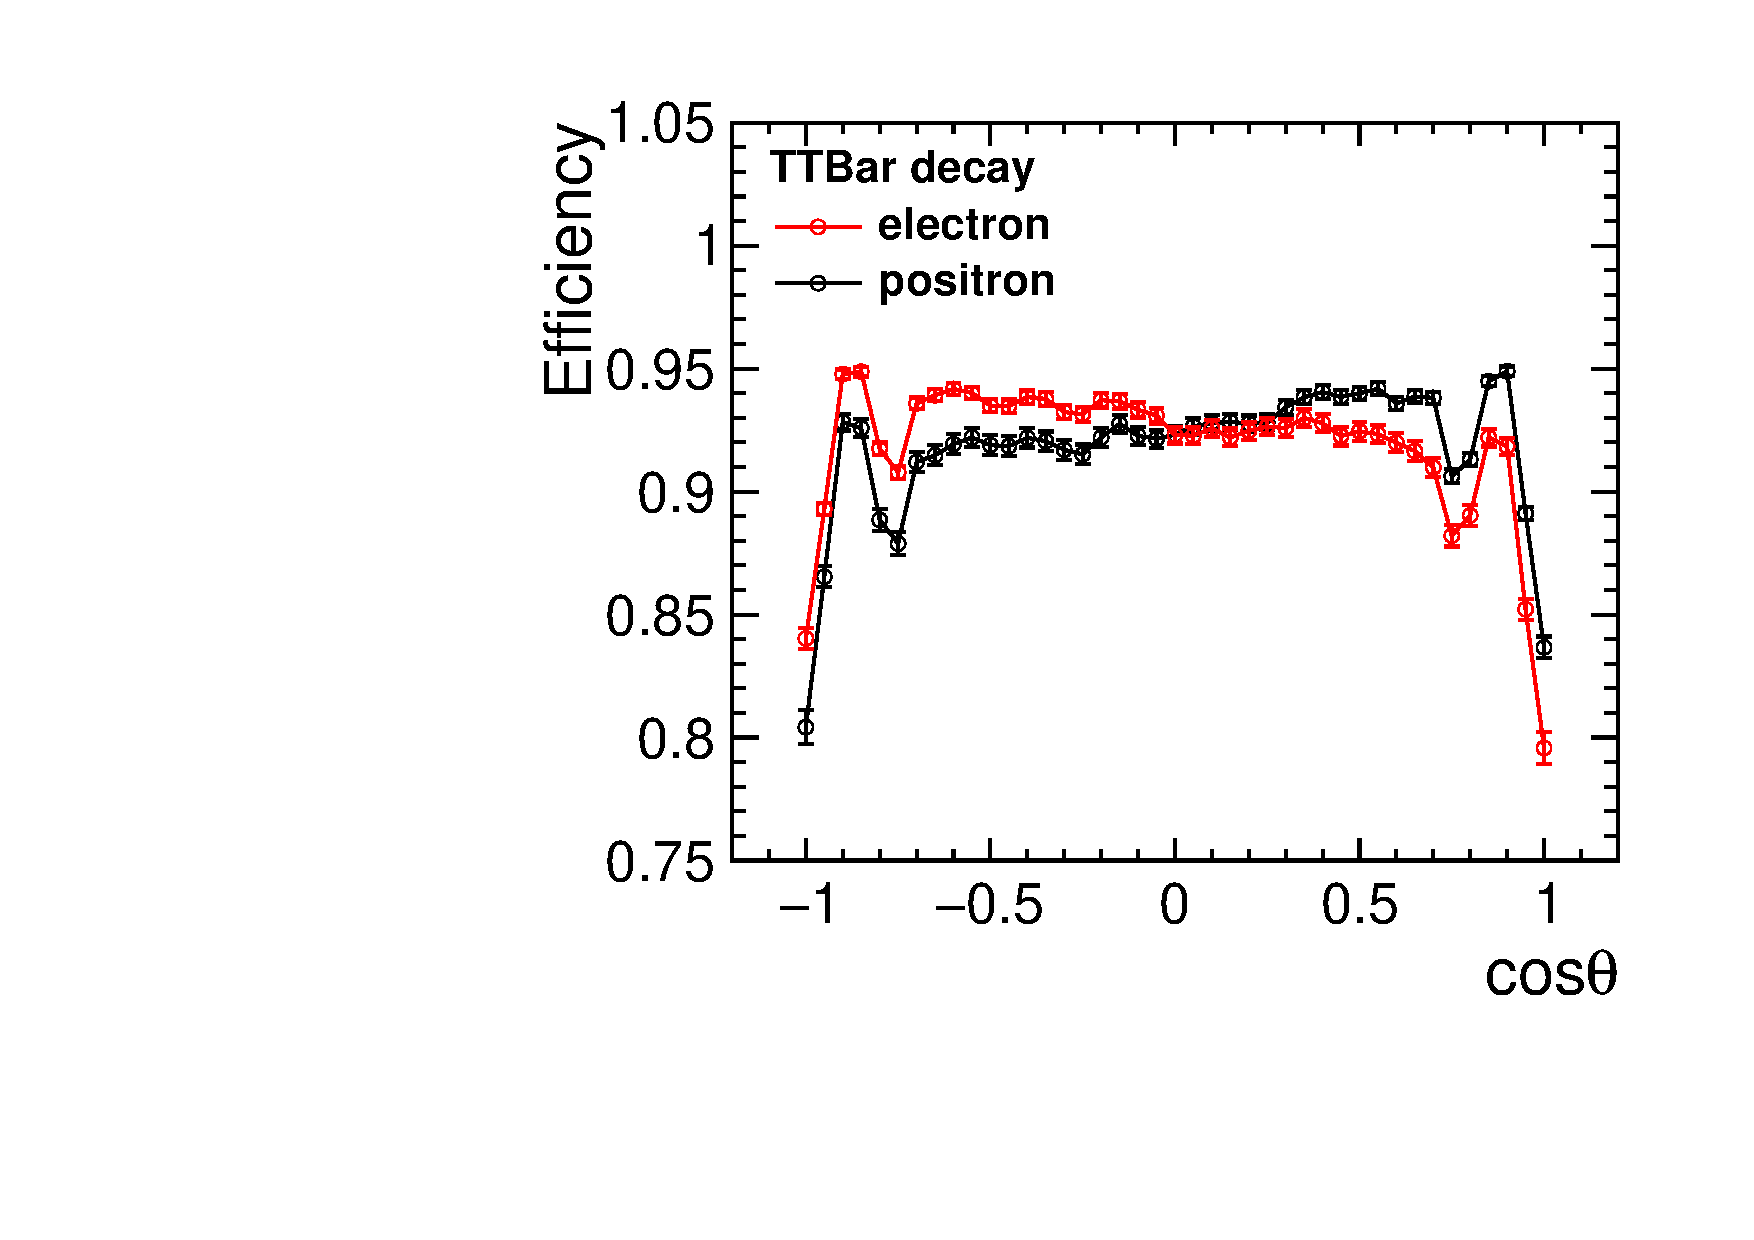
\includegraphics[width=0.99\textwidth]{TopAnalysis/figures/ElectronEfficiencys.pdf}
    \caption[Charge Tagging Efficiency]{Electrons}
    \label{fig:electronefficiency}
  \end{subfigure}%
  \begin{subfigure}{.5\textwidth}
    \centering
    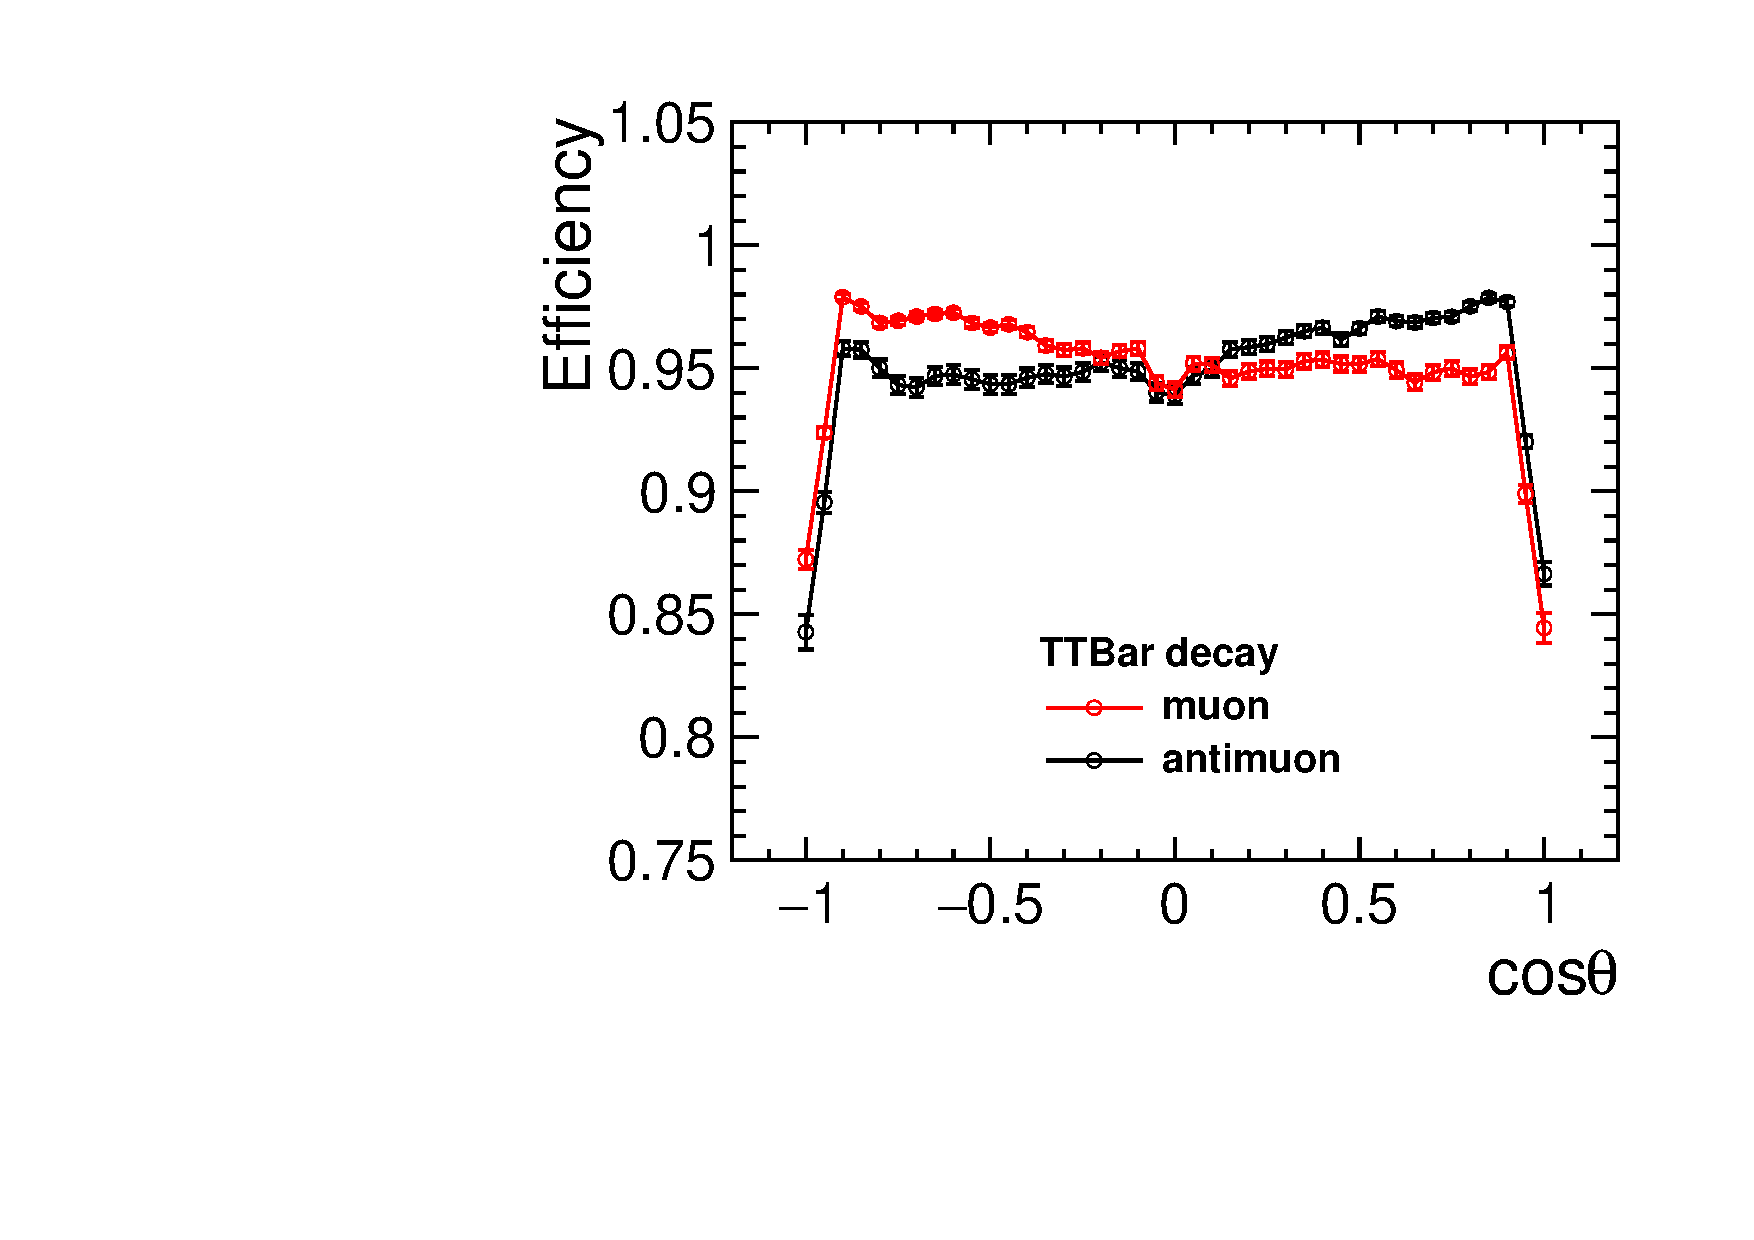
\includegraphics[width=0.99\textwidth]{TopAnalysis/figures/MuonEfficiencys.pdf}
    \caption[Charge Tagging Efficiency]{Muons}
    \label{fig:muonefficiency}
  \end{subfigure}
  \caption{Angular dependence of lepton finding for particles vs antiparticles.}
  \label{fig:chargeEfficiencies}
\end{figure}

This arises from the underlying asymmetry in the production of particles vs antiparticles due to forward-backward asymmetries. The top forward backward asymmetry means that tops are preferentially produced in one direction while antitops are produced more often in the opposite direction, however due to charge conservation this also means that the W bosons and leptons are produced asymmetrically too. Because the collisions are taking place well above the top pair production threshold, the W bosons will gain a large boost forcing them to travel in the same direction as the initial top. The polarization of the W means that the lepton will also be preferentially produced along the same direction as the W and will only be produced in the opposite direction with a lower energy. Overall this means that leptons are produced with higher energy in one direction and lower energy in the opposite direction while for antileptons this directional dependence is reversed. The effect is shown in \reffig{fig:efficiency2d} where it is seen that positrons are produced with a higher abundance and greater energy in the forward direction ($\cos\theta>0$) than the backward direction. It is known that the efficiency for reconstructing leptons at CLIC increases with energy and so the fact the energy and angle at which leptons are produced are correlated results in the asymmetric angular efficiency for correctly reconstructing the lepton. Further evidence for this theory is shown in \reffigs{fig:higgsleptons} and \ref{fig:effienciesWithCuts} which show that the asymmetry disappears when either the production mode for the leptons is symmetric or when low energy leptons are not included.

\begin{figure}
  \centering
  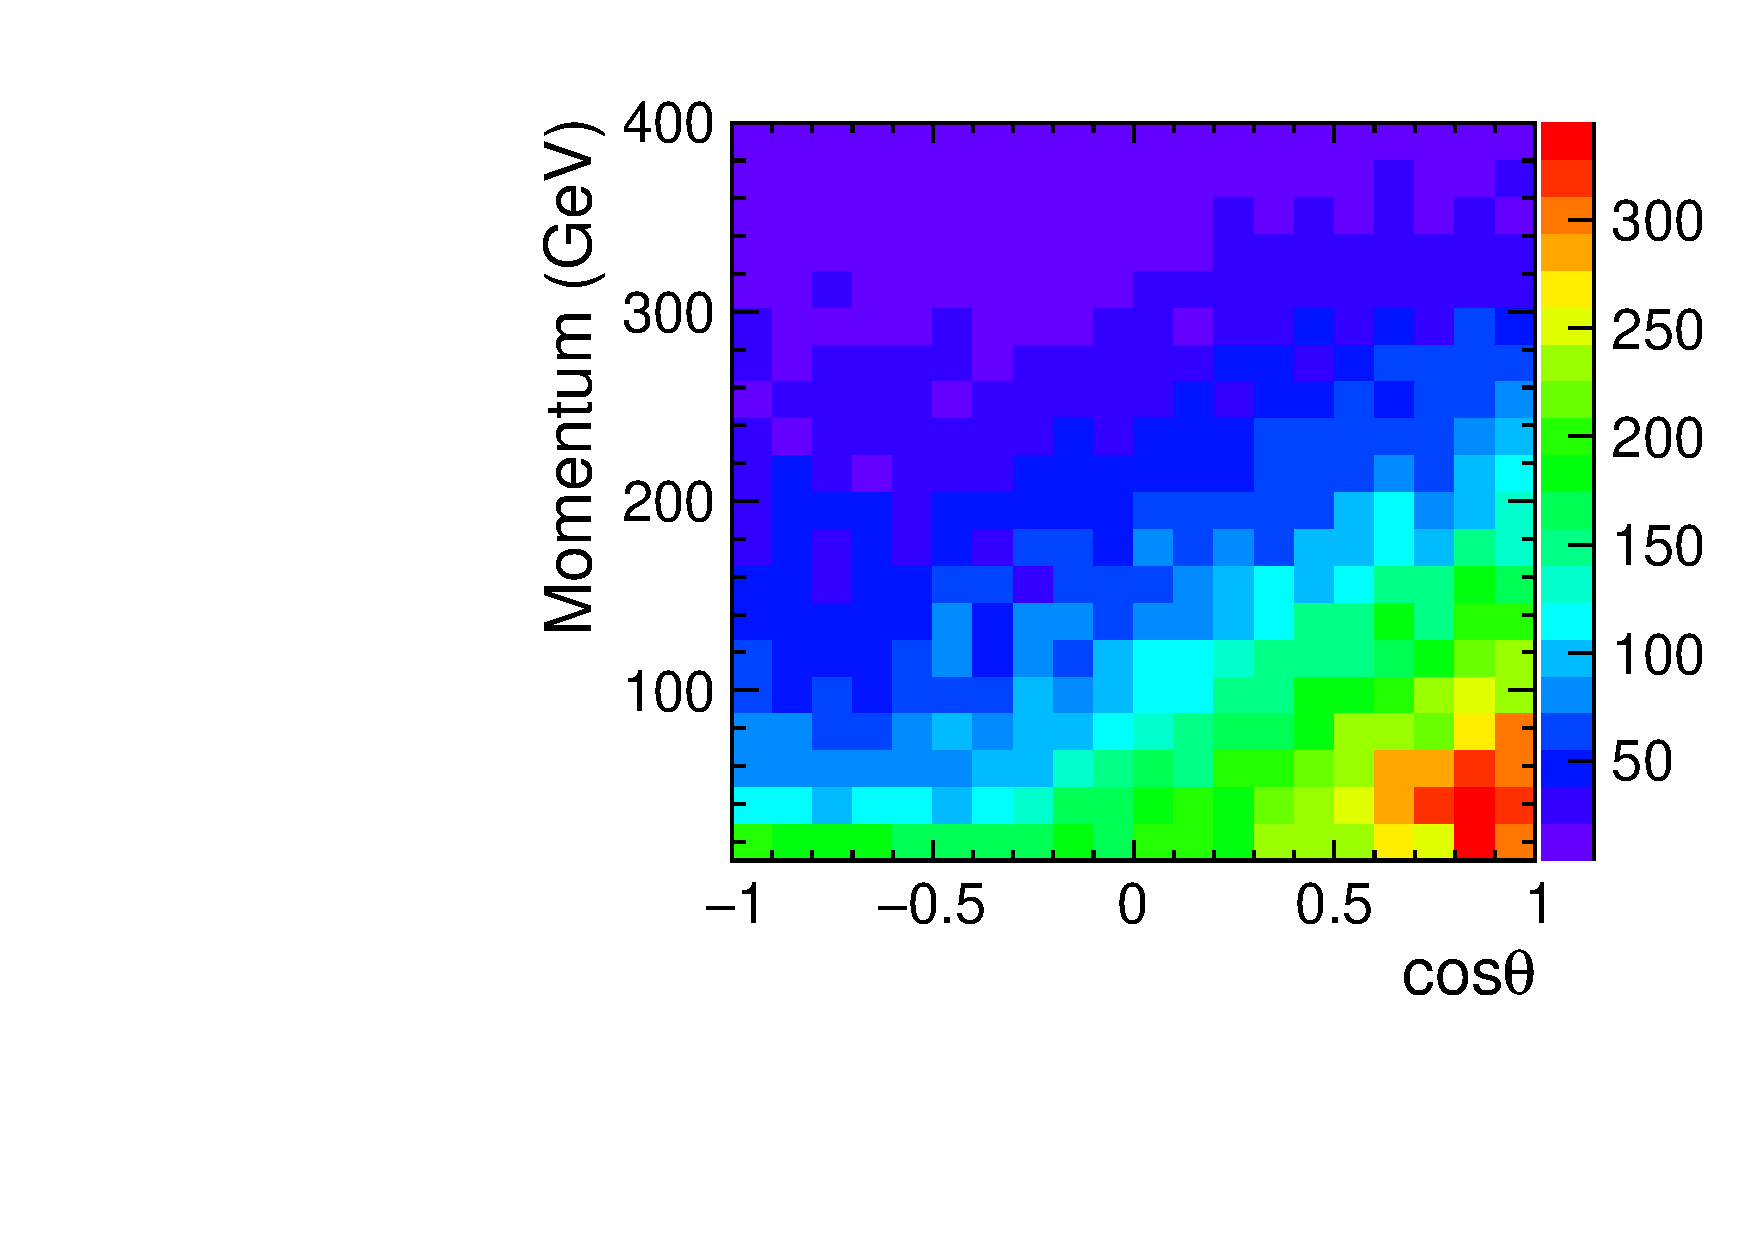
\includegraphics[width=0.6\textwidth]{TopAnalysis/figures/MomentumVsTheta.pdf}
  \caption[Lepton Momentum Vs Angle]{Correlation between lepton momentum and angle for positrons only.}
  \label{fig:efficiency2d}
\end{figure}

\begin{figure}
  \centering
  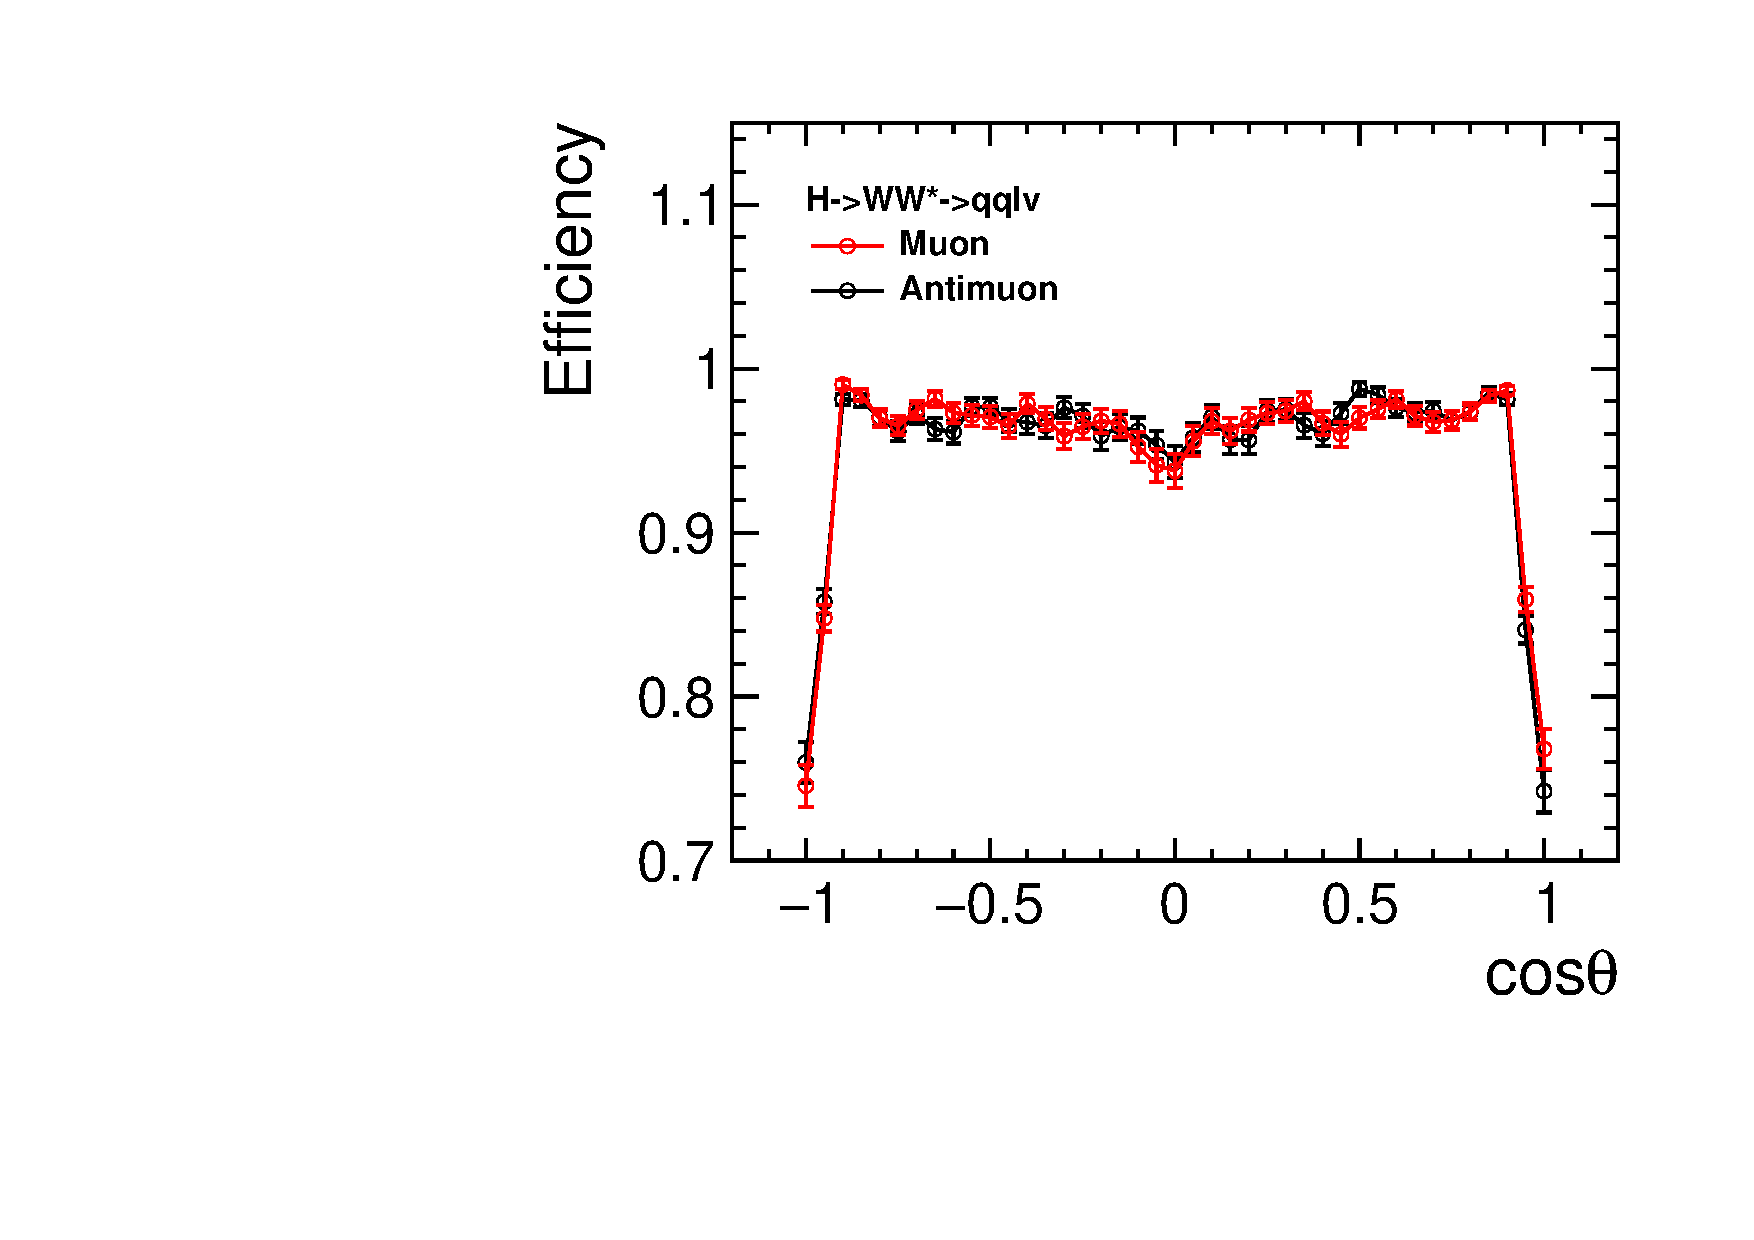
\includegraphics[width=0.8\textwidth]{TopAnalysis/figures/MuonEfficiency_Higgs.pdf}
  \caption[Lepton efficiency for $ee\rightarrow H\nu\nu,H \rightarrow WW\rightarrow qql\nu$ ]{Charge tagging efficiency for $ee\rightarrow H\nu\nu,H \rightarrow WW\rightarrow qql\nu$. The efficiency is seen to be symmetric for particles and antiparticles when they are produced with the same initial angular distribution.}
  \label{fig:higgsleptons}
\end{figure}

\begin{figure}
  \centering
  \begin{subfigure}{.5\textwidth}
    \centering
    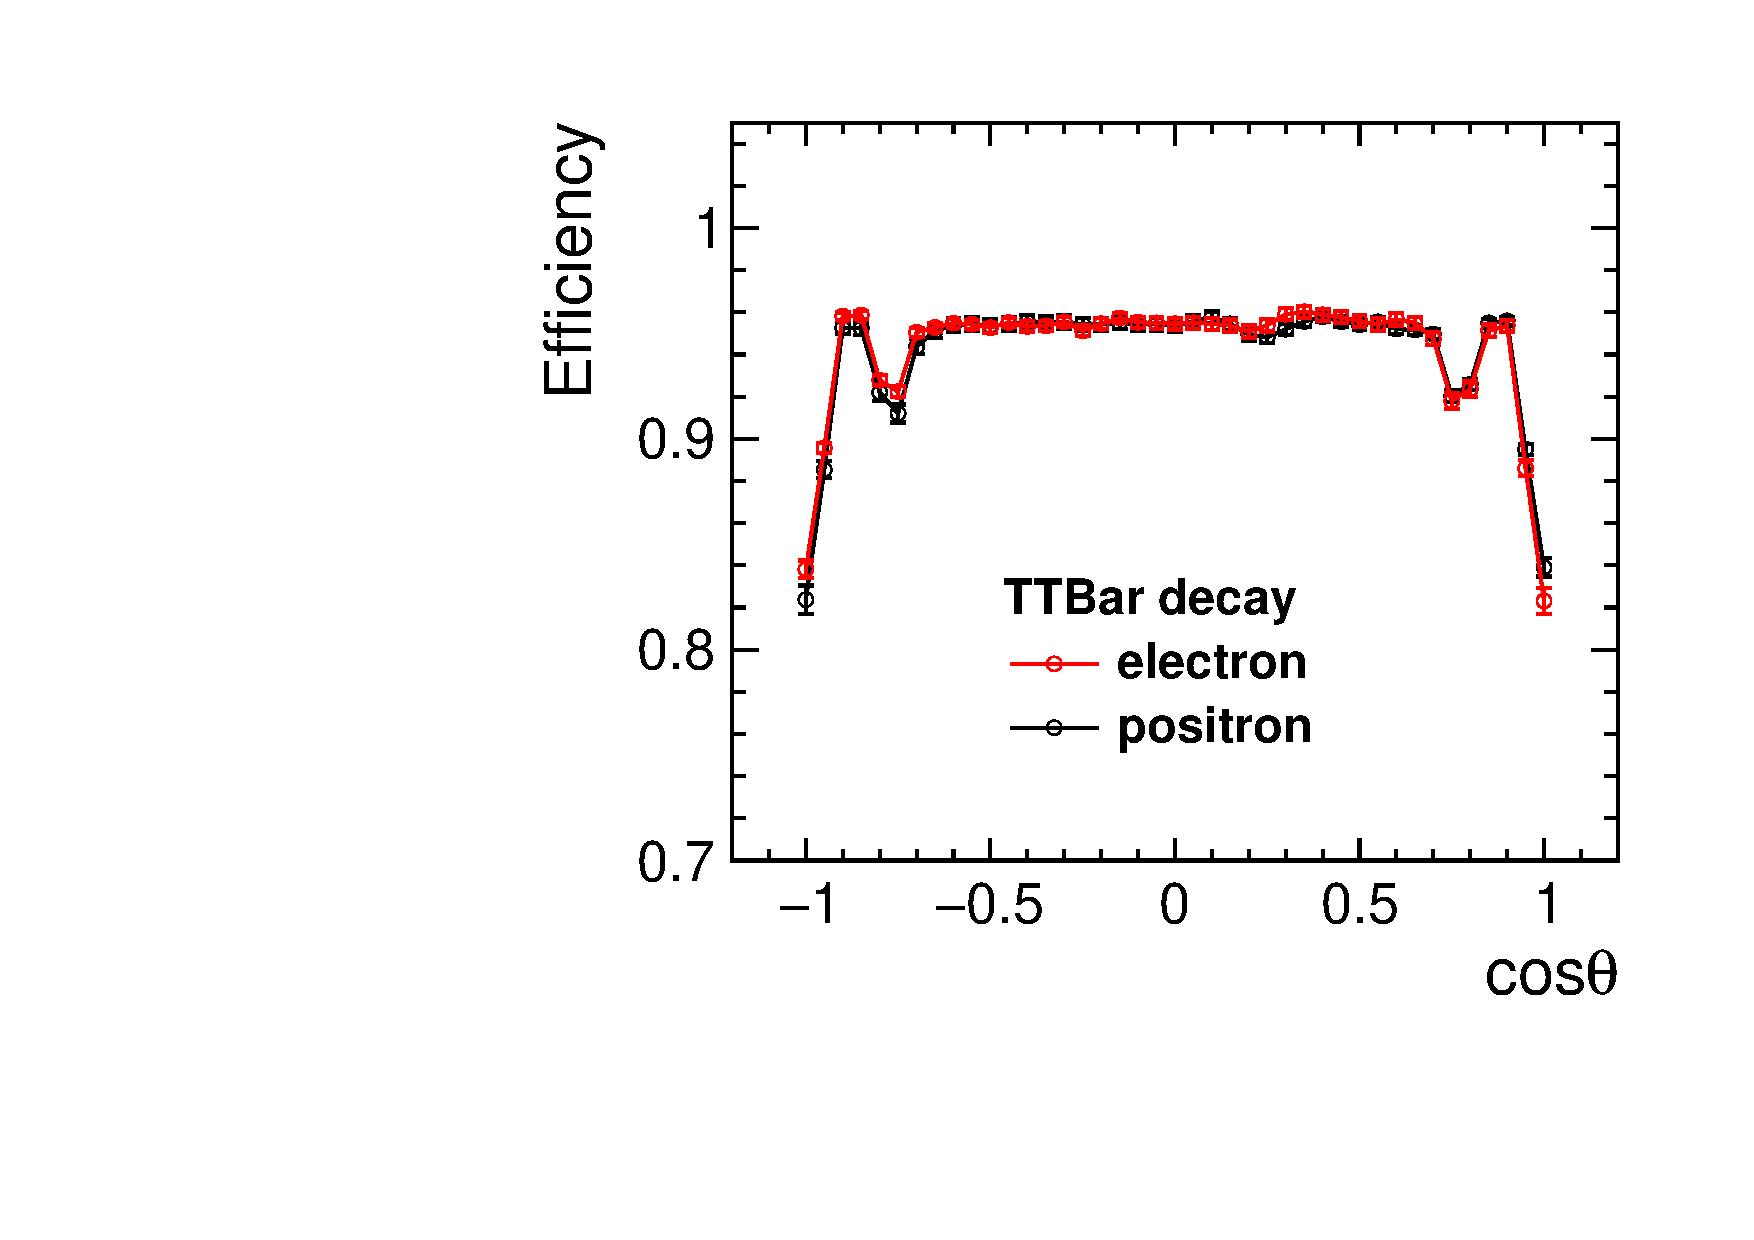
\includegraphics[width=0.99\textwidth]{TopAnalysis/figures/ElectronEfficiencys_20GeVMCCut.pdf}
    \caption[Charge Tagging Efficiency]{Electrons}
  \end{subfigure}%
  \begin{subfigure}{.5\textwidth}
    \centering
    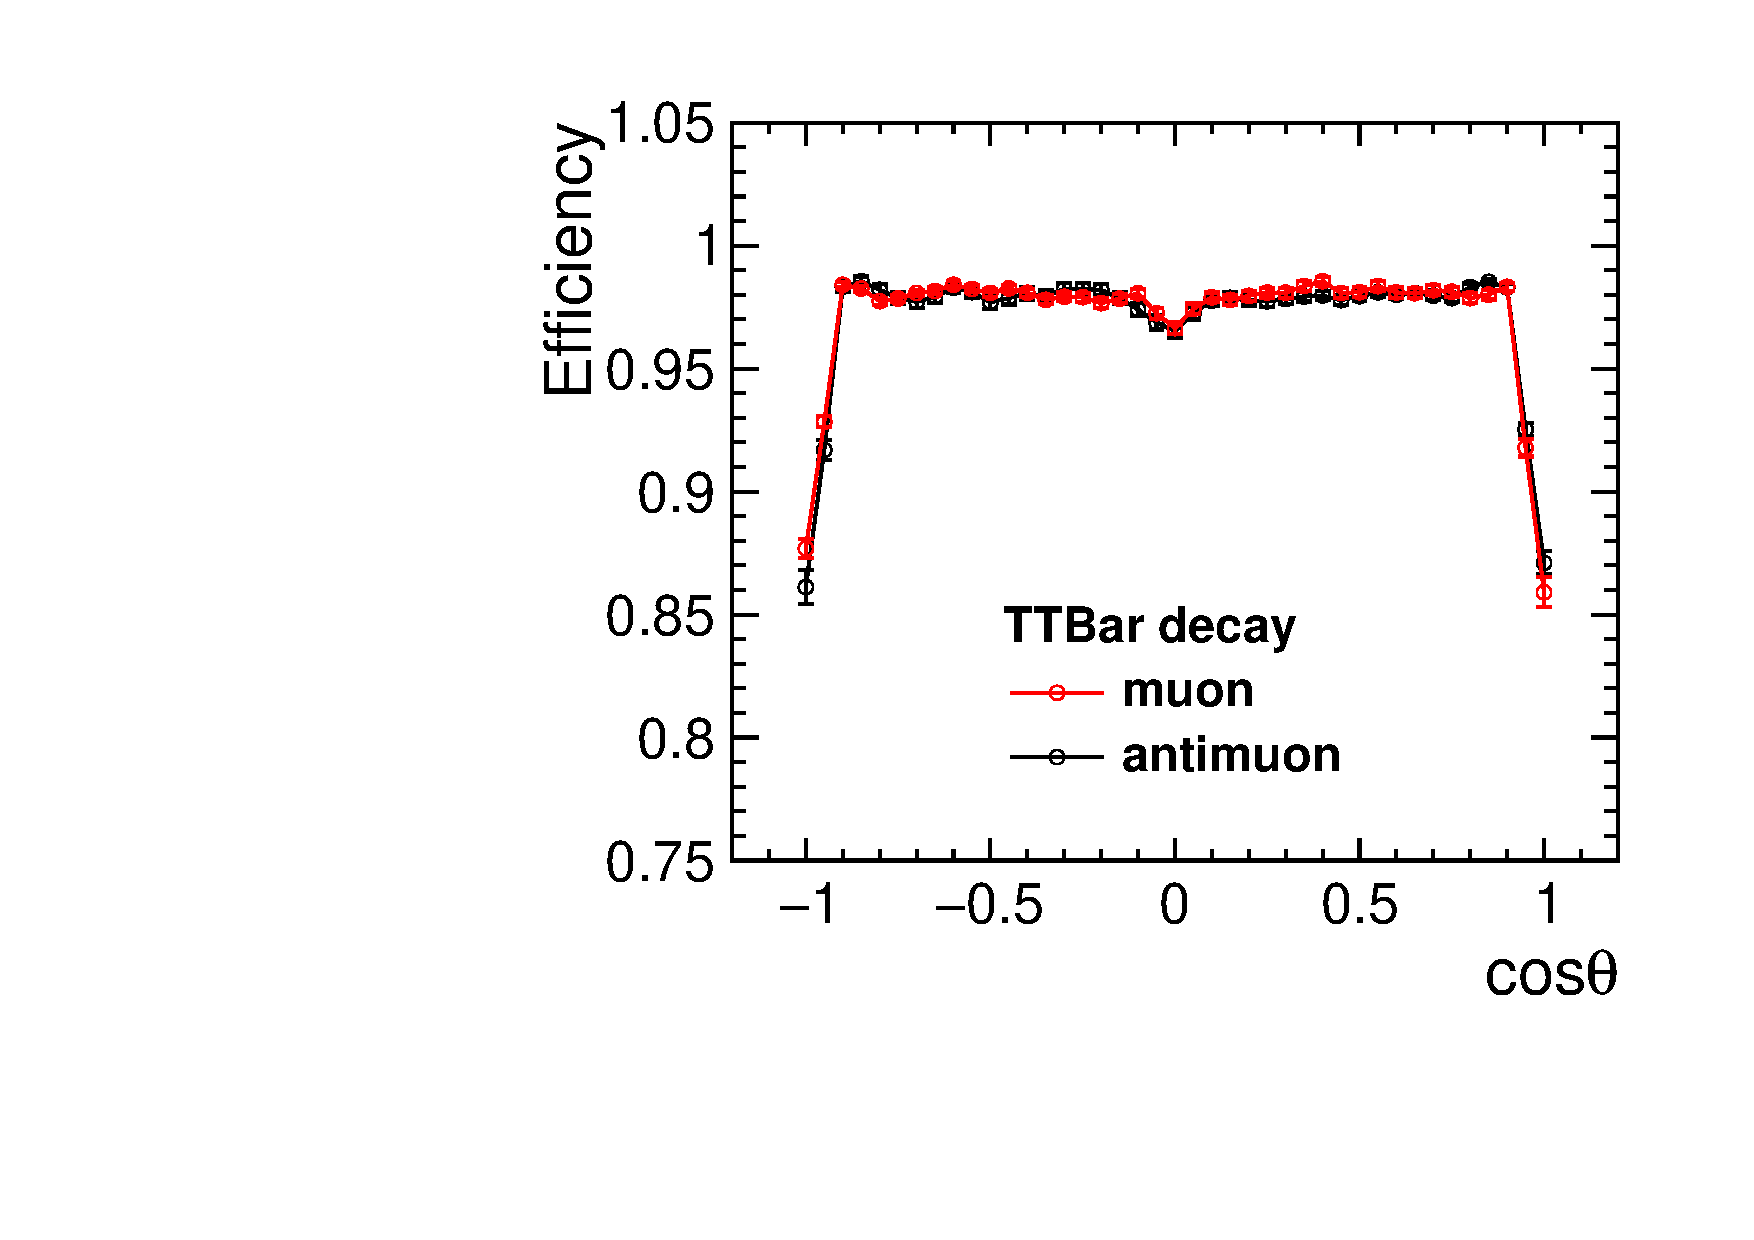
\includegraphics[width=0.99\textwidth]{TopAnalysis/figures/MuonEfficiencys_20GeVMCCut.pdf}
    \caption[Charge Tagging Efficiency]{Muons}
  \end{subfigure}
  \caption[Charge Tagging Efficiency After 20 GeV Lepton Momentum Cut]{Charge tagging efficiency after 20~GeV lepton momentum cut. The efficiency is seen to be symmetric for leptons with momentum $>$ 20~GeV.}
  \label{fig:effienciesWithCuts}
\end{figure}


\subsection{Fat Jet Finding}

\begin{figure}
  \centering
  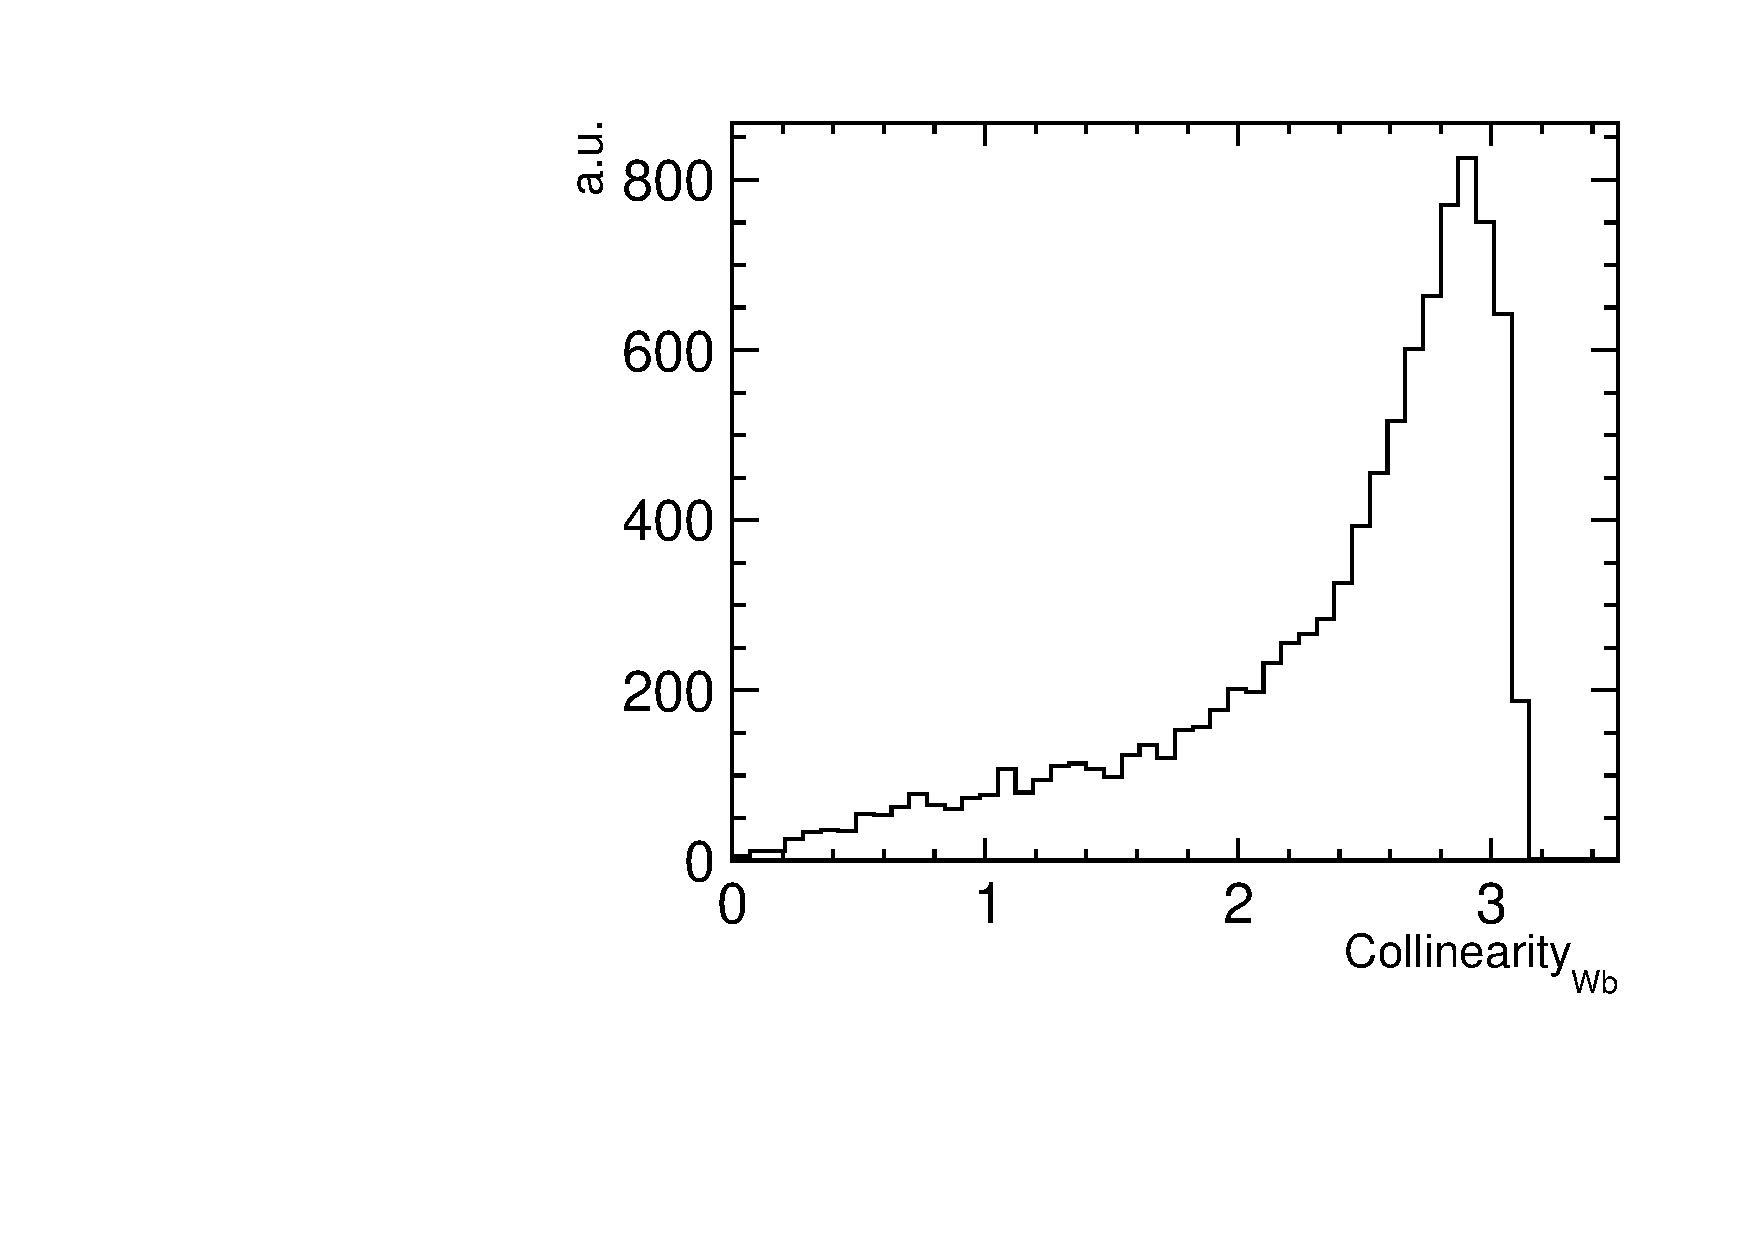
\includegraphics[width=0.6\textwidth]{TopAnalysis/figures/WBCollinearity.pdf}
  \caption[Separation between W and b jet from top decay]{Separation between W and b jets from top decays. The pair are typically too collimated to allow the b-jet and the pair of jets from the W decay to be successfully resolved into three distinct objects.}
  \label{fig:Collimated}
\end{figure}

Jet reconstruction was performed using the FastJet package \cite{Cacciari:2011ma}. Due to the high centre-of-mass of the collisions relative to the top mass, the tops produced are highly boosted and produce highly collimated decay products (see \reffig{fig:Collimated}.) This means it is typically not possible to resolve the decay products from the hadronically decaying top into three objects corresponding to the b-jet and light quark jets from the W decay. As a result, an alternative approach to jet reconstruction is considered based on the concept of fat jets, a technique already being used at the LHC\cite{Miller:2011qg}. Fat jets are large radius jets and are used to cluster groups of jets that cannot be accurately resolved individually into one larger jet. For the purpose of this analysis the events are clustered into two fat jets which should correspond to the b-jet from the leptonically decaying top and to the collective decay products of the hadronically decaying top. The mass and substructure (see \refsec{Event Selection}) of these fat jets can then be used to distinguish genuine top events from backgrounds. Two jet algorithms were considered for reconstructing the fat jets: the longitudinally invariant kt algorithm \cite{Cacciari:2008gp} and Valencia algorithm \cite{Boronat:2014hva}. The kt algorithm is already extensively used at hadron colliders while the Valencia algorithm is a newer variant of this designed for future lepton colliders that offers improved performance in handling beam related backgrounds. A full description of the kt algorithm is already given in \refsec{higgsjetfinding} so here we will only describe the Valencia algorithm. Overall the Valencia algorithm is similar to the kt algorithm, however the key differences are that the inter-particle distance and beam distance are redefined as:

\begin{equation}
d_{ij}=min(E_i^{2\beta},E_j^{2\beta})(1-cos\theta_{ij})/R^2
\end{equation}
\begin{equation}
d_{iB}=p_T^{2\gamma}E^{2(\beta - \gamma)},
\end{equation}

where $R$ is the usual jet radius defined in the same way as for the kt algorithm and $\beta$ and $\gamma$ are additional parameters that can be used to tune how the algorithm behaves for particles approaching the beam line. \reffig{fig:valenciaPerformance} shows how the ratio $d_{ij}/d_{iB}$ develops for a pair of particles produced with fixed energy and angular separation as a function of their polar angle for multiple $\beta$ factors. One can see that a higher $\beta$ factor introduces a larger penalty for approaching the beam line leading to a decreased chance for the particles to be merged into a jet.

\begin{figure}
  \centering
  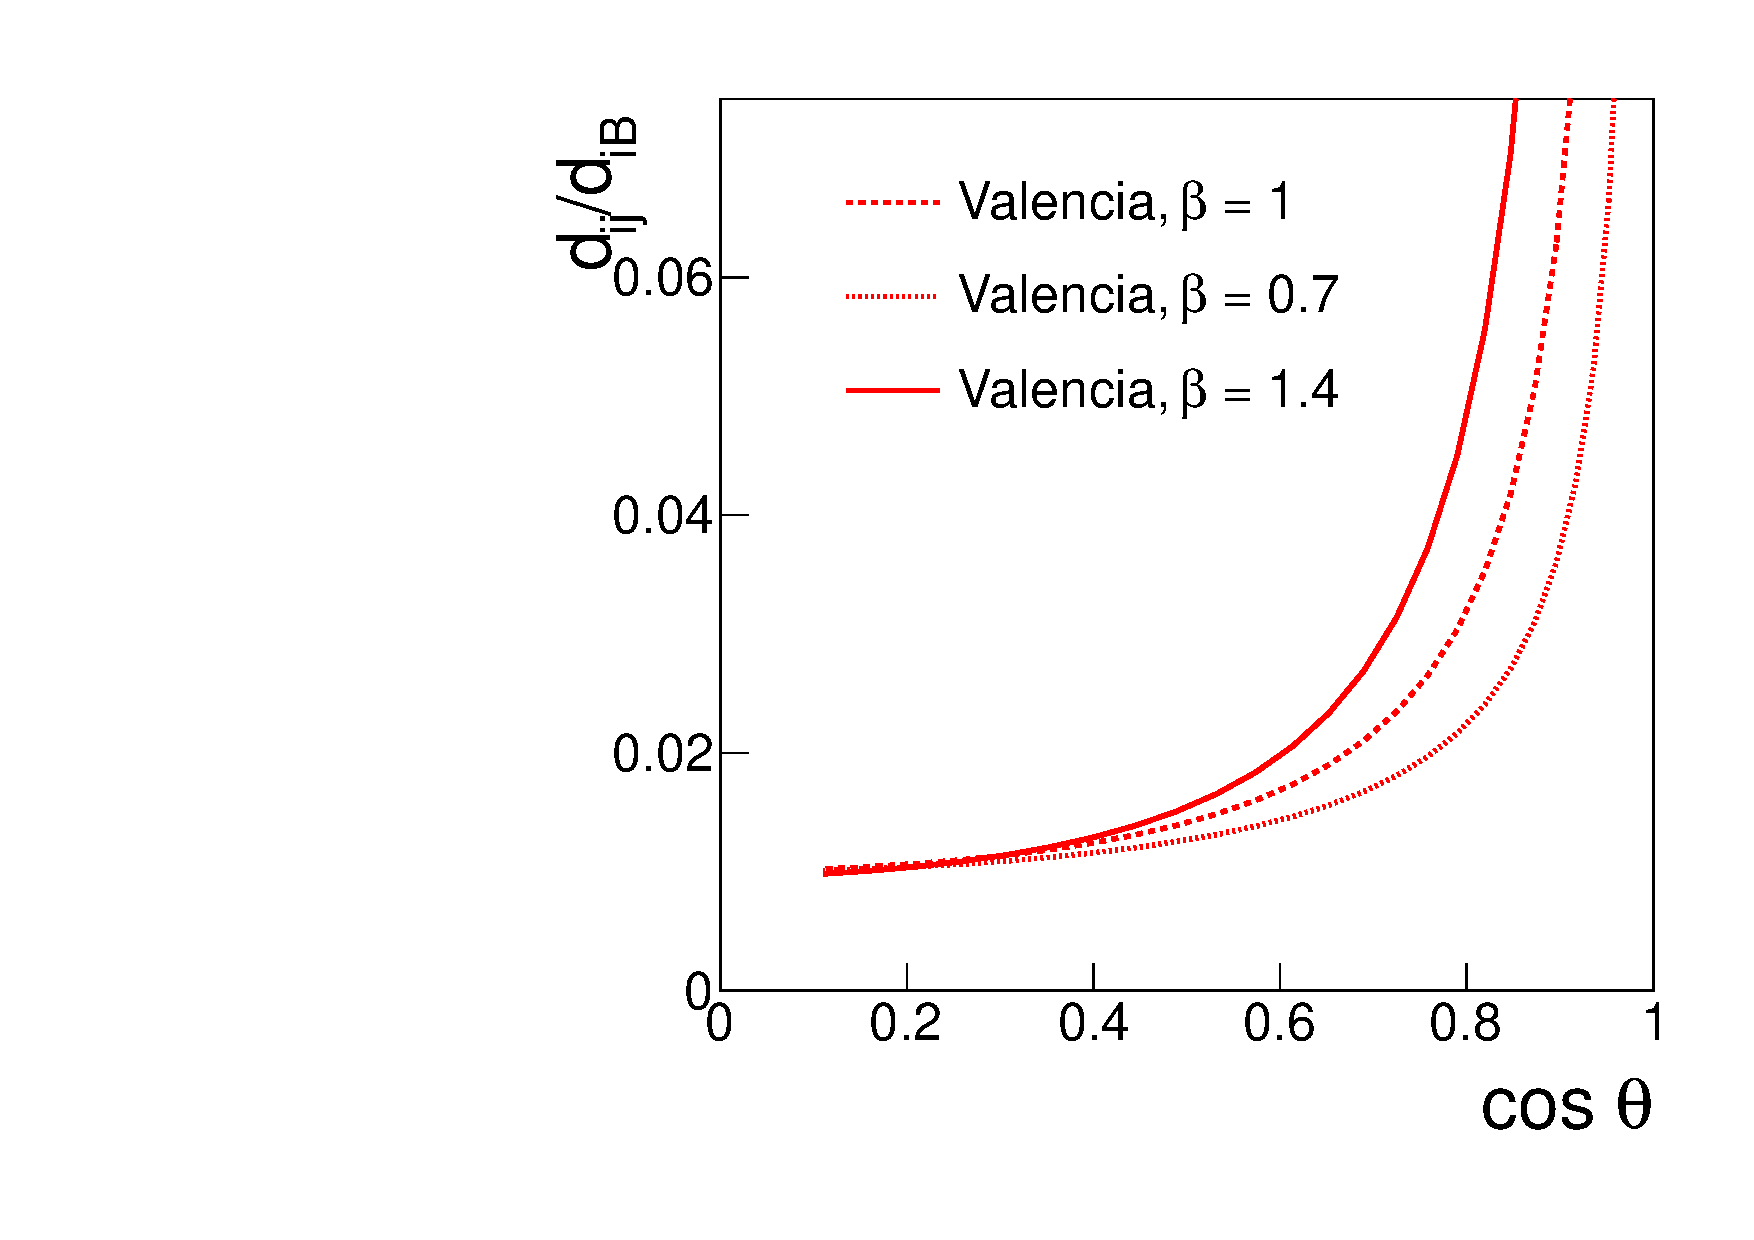
\includegraphics[width=0.6\textwidth]{TopAnalysis/figures/distance_ratio_vlc.pdf}
  \caption[Effect of the Valencia $\beta$ parameter]{Effect of the Valencia $\beta$ parameter on $d_{ij}/d_{iB}$ for a pair of particles produced at a fixed energy and angular separation as a function of their polar angle\cite{Boronat:2014hva}.}
  \label{fig:valenciaPerformance}
\end{figure}

The performance of both algorithms was evaluated based on their ability to reconstruct the mass of the hadronically decaying top as shown in figure \reffig{fig:jetfinding}. For both algorithms it is seen that at higher R the resolution on the top mass degrades while for lower $R$ sub-peaks start to appear in the mass distribution corresponding to partial reconstructions of the top (either a W boson or single quark). The kt algorithm is seen to produce a consistently broader distribution in the top mass. Placing a cut on the collision energy of E $>$ 1.2~TeV reveals that these lower mass peaks only occur for lower collision energies where the tops will no longer be produced back to back and their decay products will be less collimated. As a result the fat jet finding can merge components from both the hadronic and leptonic tops into each jet. This analysis will be focusing on reconstructing the most boosted tops. As a result the Valencia algorithm is preferred due to its better mass resolution. Performance for less boosted top decays might be improved by examining the performance of a more conventional jet analysis looking to resolve all four individual quarks whenever the fat jet finding produces jets outside the top mass window. This possibility is not examined here but represents a potential improvement for low $\sqrt{s'}$ events. Here the Valencia algorithm with $R$=1.5, $\beta$=1 and $\gamma$=1 is chosen as the optimal jet reconstruction method to provide a balance between mass resolution and the frequency of partial reconstructions. 

\begin{figure}
  \centering
  \begin{subfigure}{1\textwidth}
    \centering
    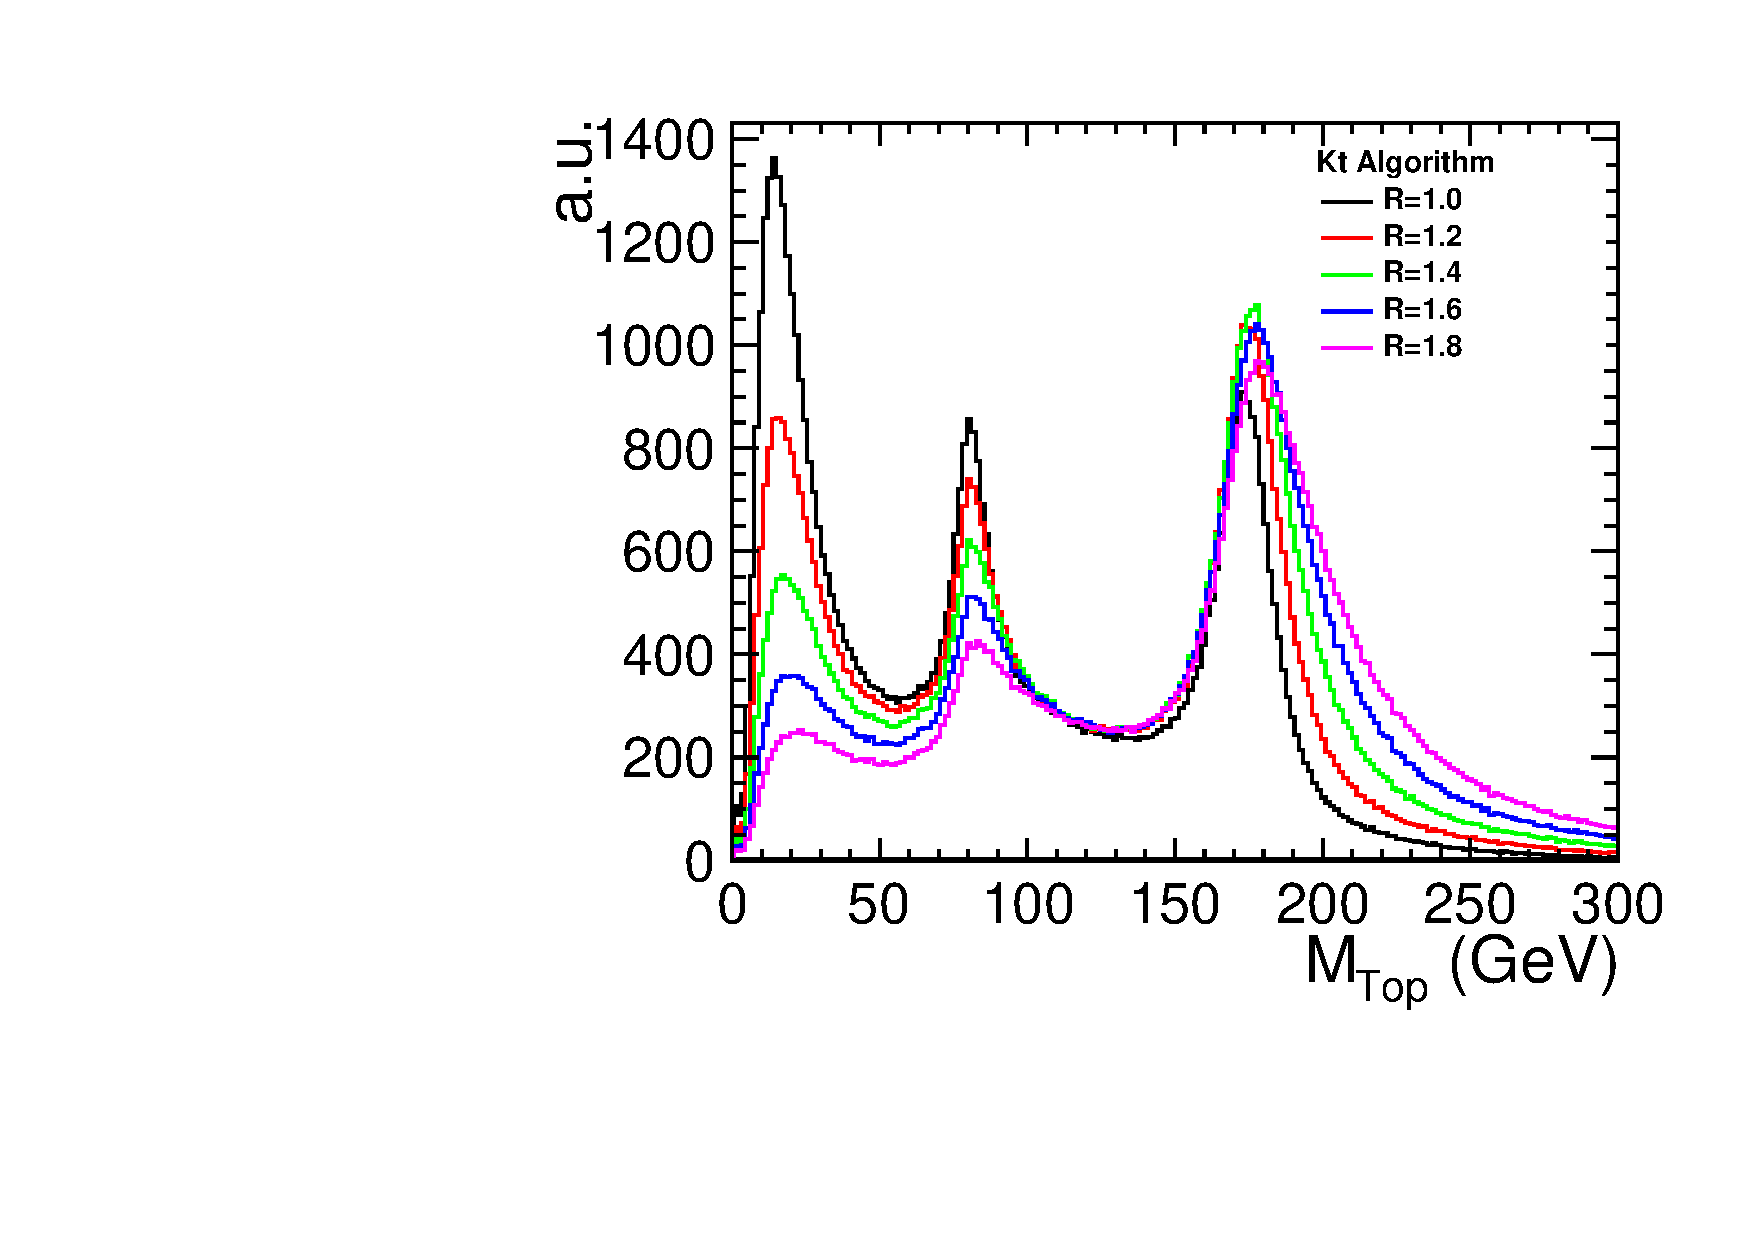
\includegraphics[width=0.8\textwidth]{TopAnalysis/figures/ComparisonKt.pdf}
    \caption[kt algorithm]{kt algorithm}
  \end{subfigure}
  \begin{subfigure}{1\textwidth}
    \centering
    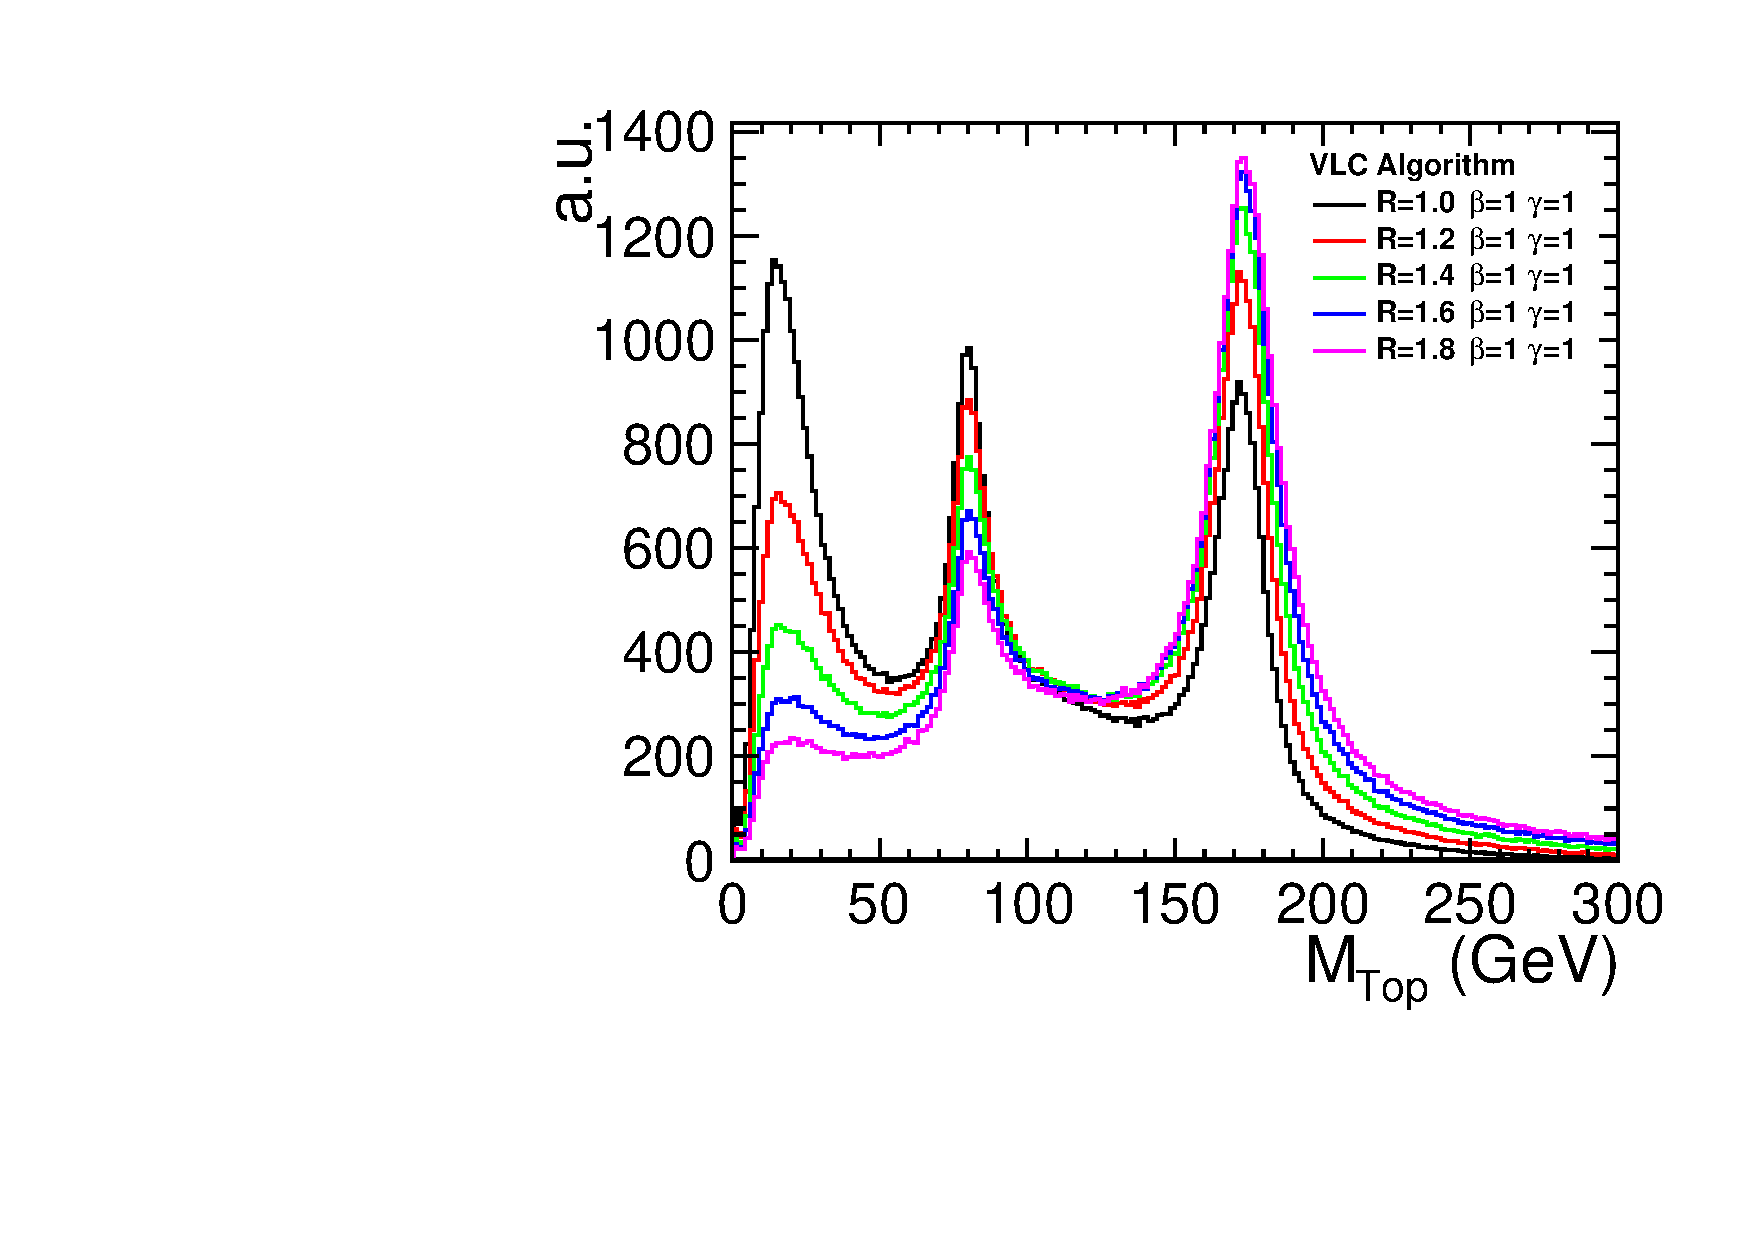
\includegraphics[width=0.8\textwidth]{TopAnalysis/figures/ComparisonVLC.pdf}
    \caption[Valencia algorithm]{Valencia algorithm}
  \end{subfigure}
  \caption[Performance of jet finding algorithms for reconstructing the top mass]{Performance of both jet finding algorithms for reconstructing the top mass for various parameter settings. }
  \label{fig:jetfinding}
\end{figure}


\begin{figure}
  \centering
  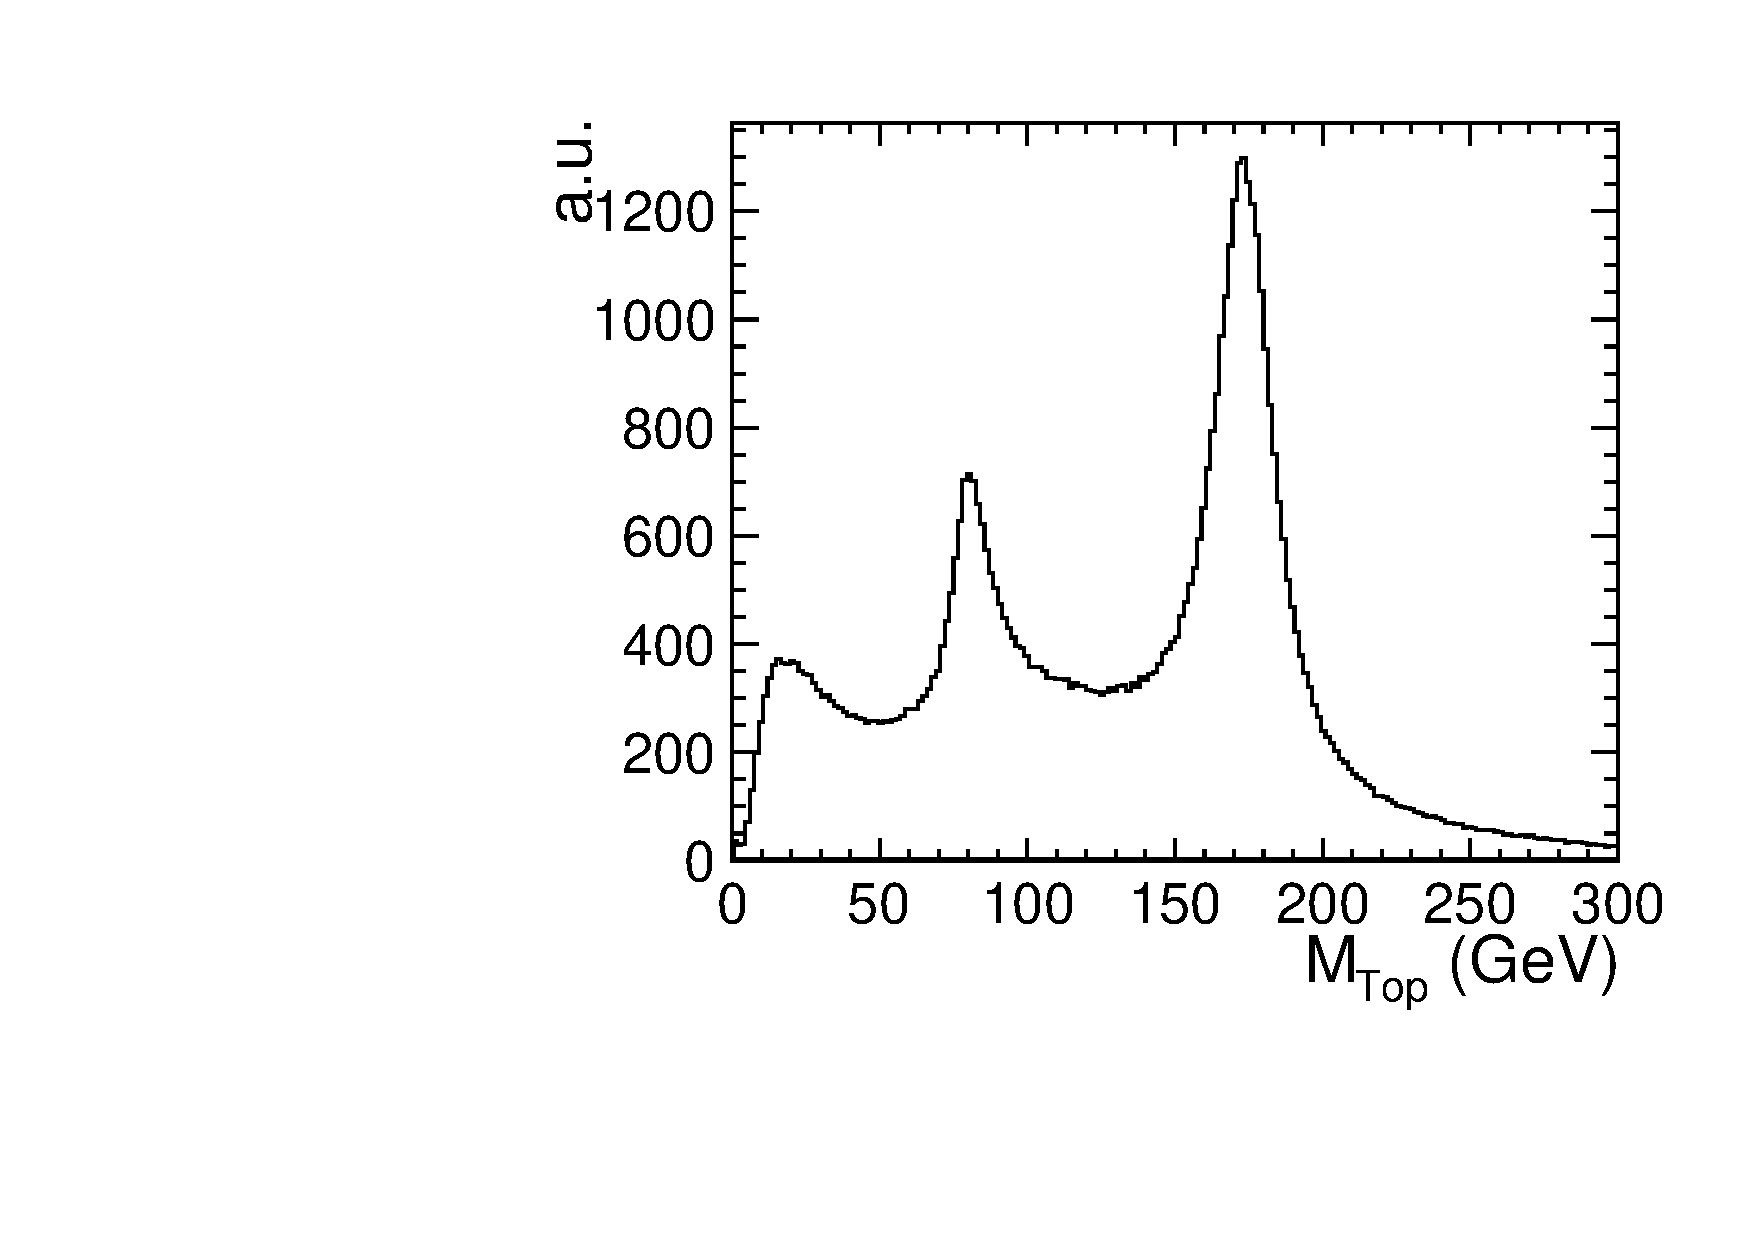
\includegraphics[width=0.7\textwidth]{TopAnalysis/figures/TopMass_EOver1200.pdf}
  \caption[Performance of Valencia algorithm for high energy events]{Reconstructed top mass for the Valencia algorithm in events close to the nominal collision energy (E $>$ 1.2~TeV).}
  \label{fig:highEValencia}
\end{figure}


\subsubsection{Jet Association}
\label{sec:jetassociation}
\begin{figure}
  \centering
  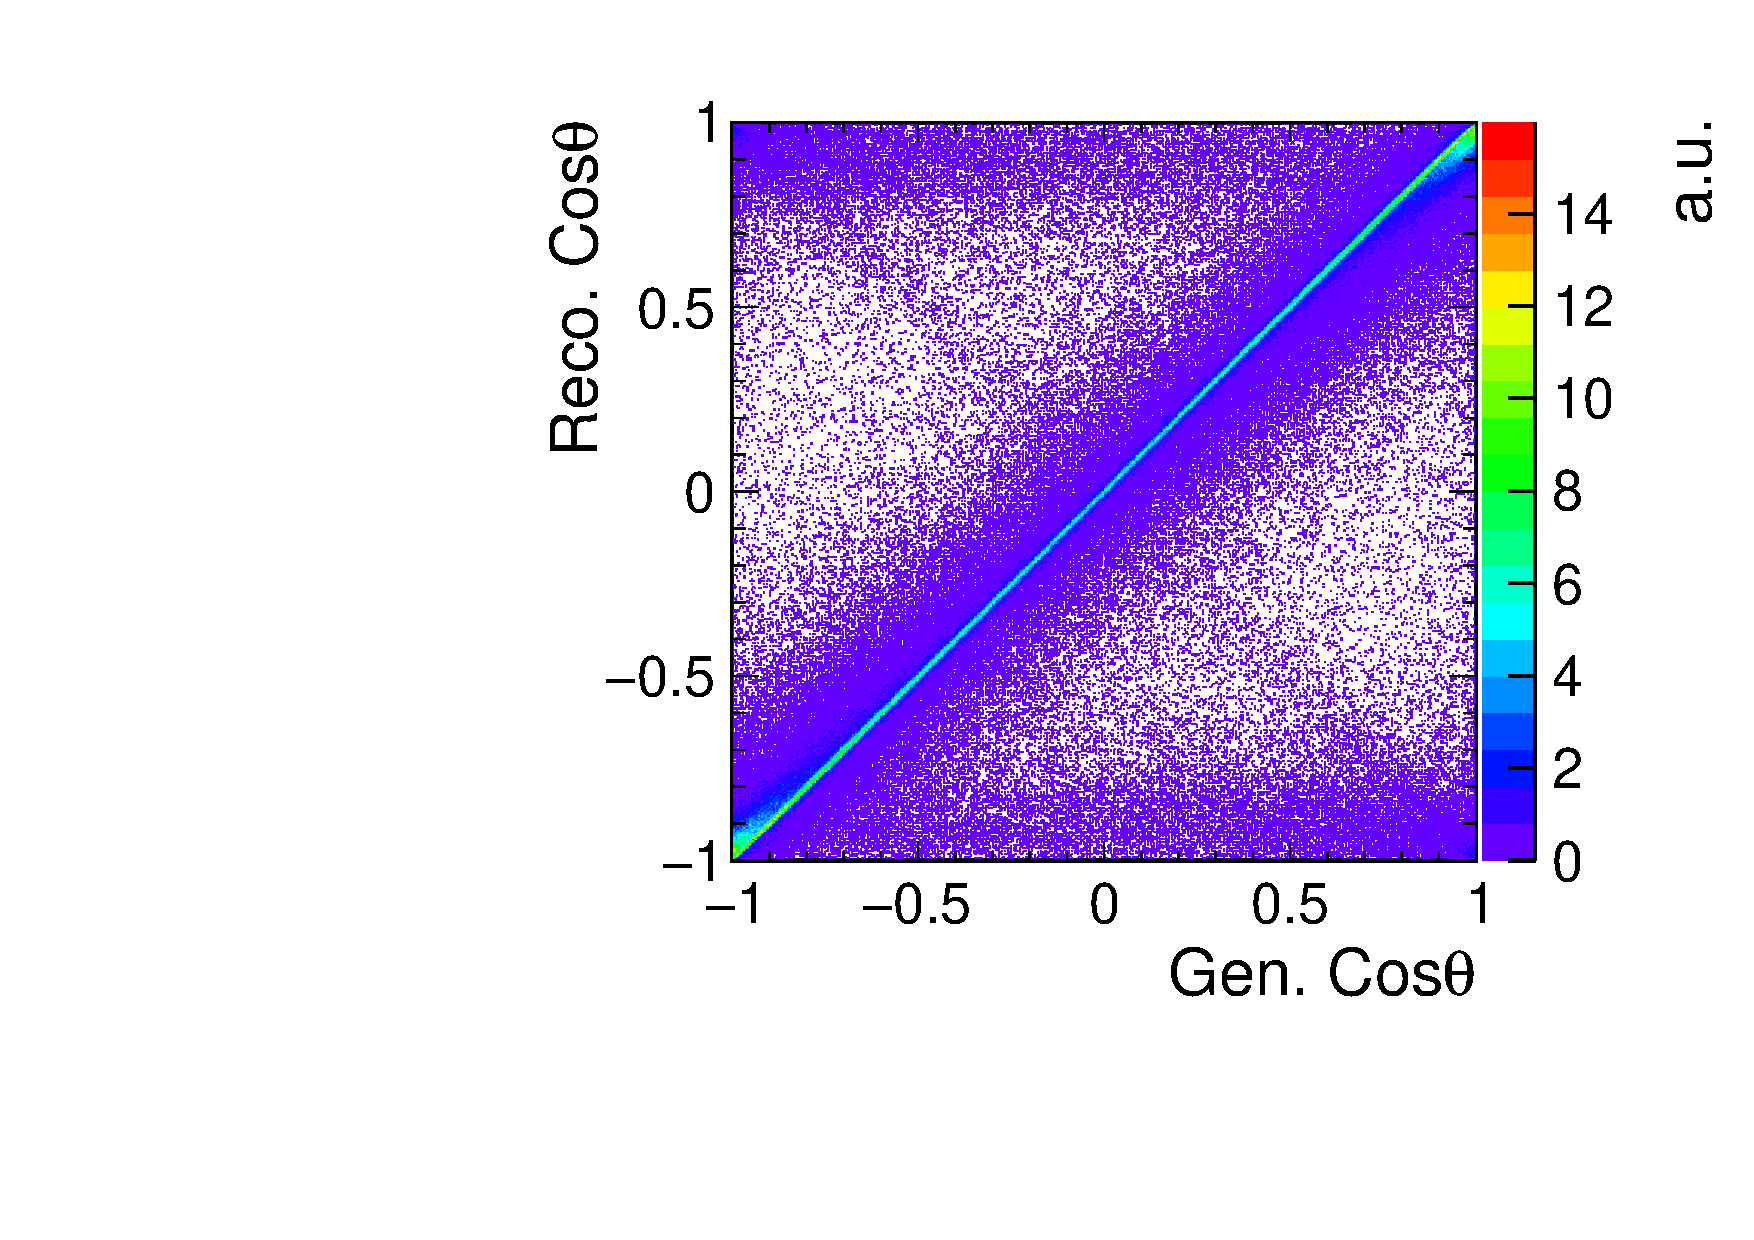
\includegraphics[width=0.7\textwidth]{TopAnalysis/figures/CosThetaRecoVsMC.pdf}
  \caption[Comparison of reconstructed top decay angle to generator level]{Comparison of reconstructed top decay angle to generator level. A strong correlation is seen over most of the range, however this starts to break down for large angles of $\mid \cos\theta \mid>0.9$ where non-negligible off diagonal contributions are seen.}
  \label{fig:2djetangle}
\end{figure}

\begin{figure}
  \centering
  \begin{subfigure}{.5\textwidth}
    \centering
    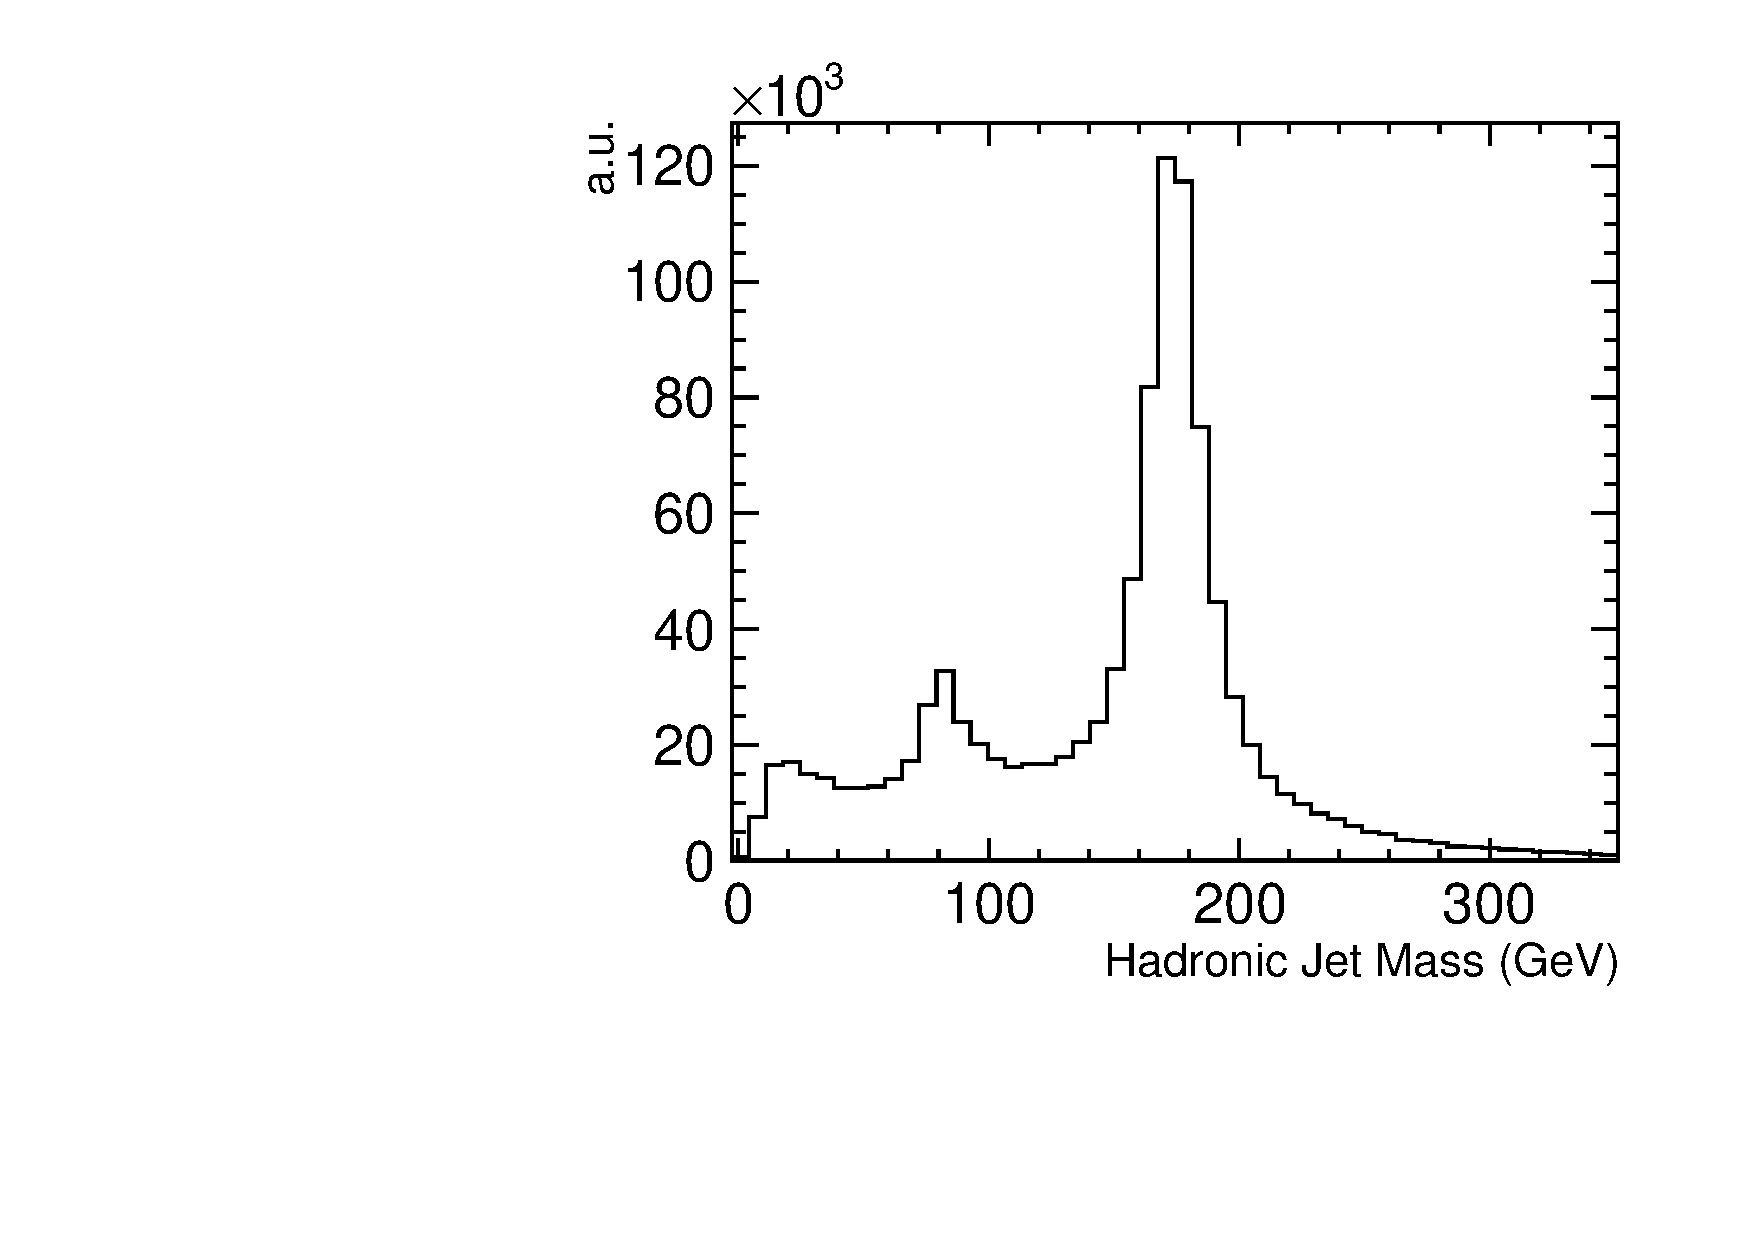
\includegraphics[width=1.0\textwidth]{TopAnalysis/figures/TopMassDiagonal.pdf}
  %  \caption[$\mid\frac{cos\theta_{Reco}}{cos\theta_{Generator}}\mid >1$]{Fat jet mass when $\mid\frac{cos\theta_{Reco}}{cos\theta_{Generator}}\mid >1$, on diagonal regions of fig \ref{fig:2djetangle}.}
  \end{subfigure}%
  \begin{subfigure}{.5\textwidth}
    \centering\captionsetup{width=.8\linewidth}%
    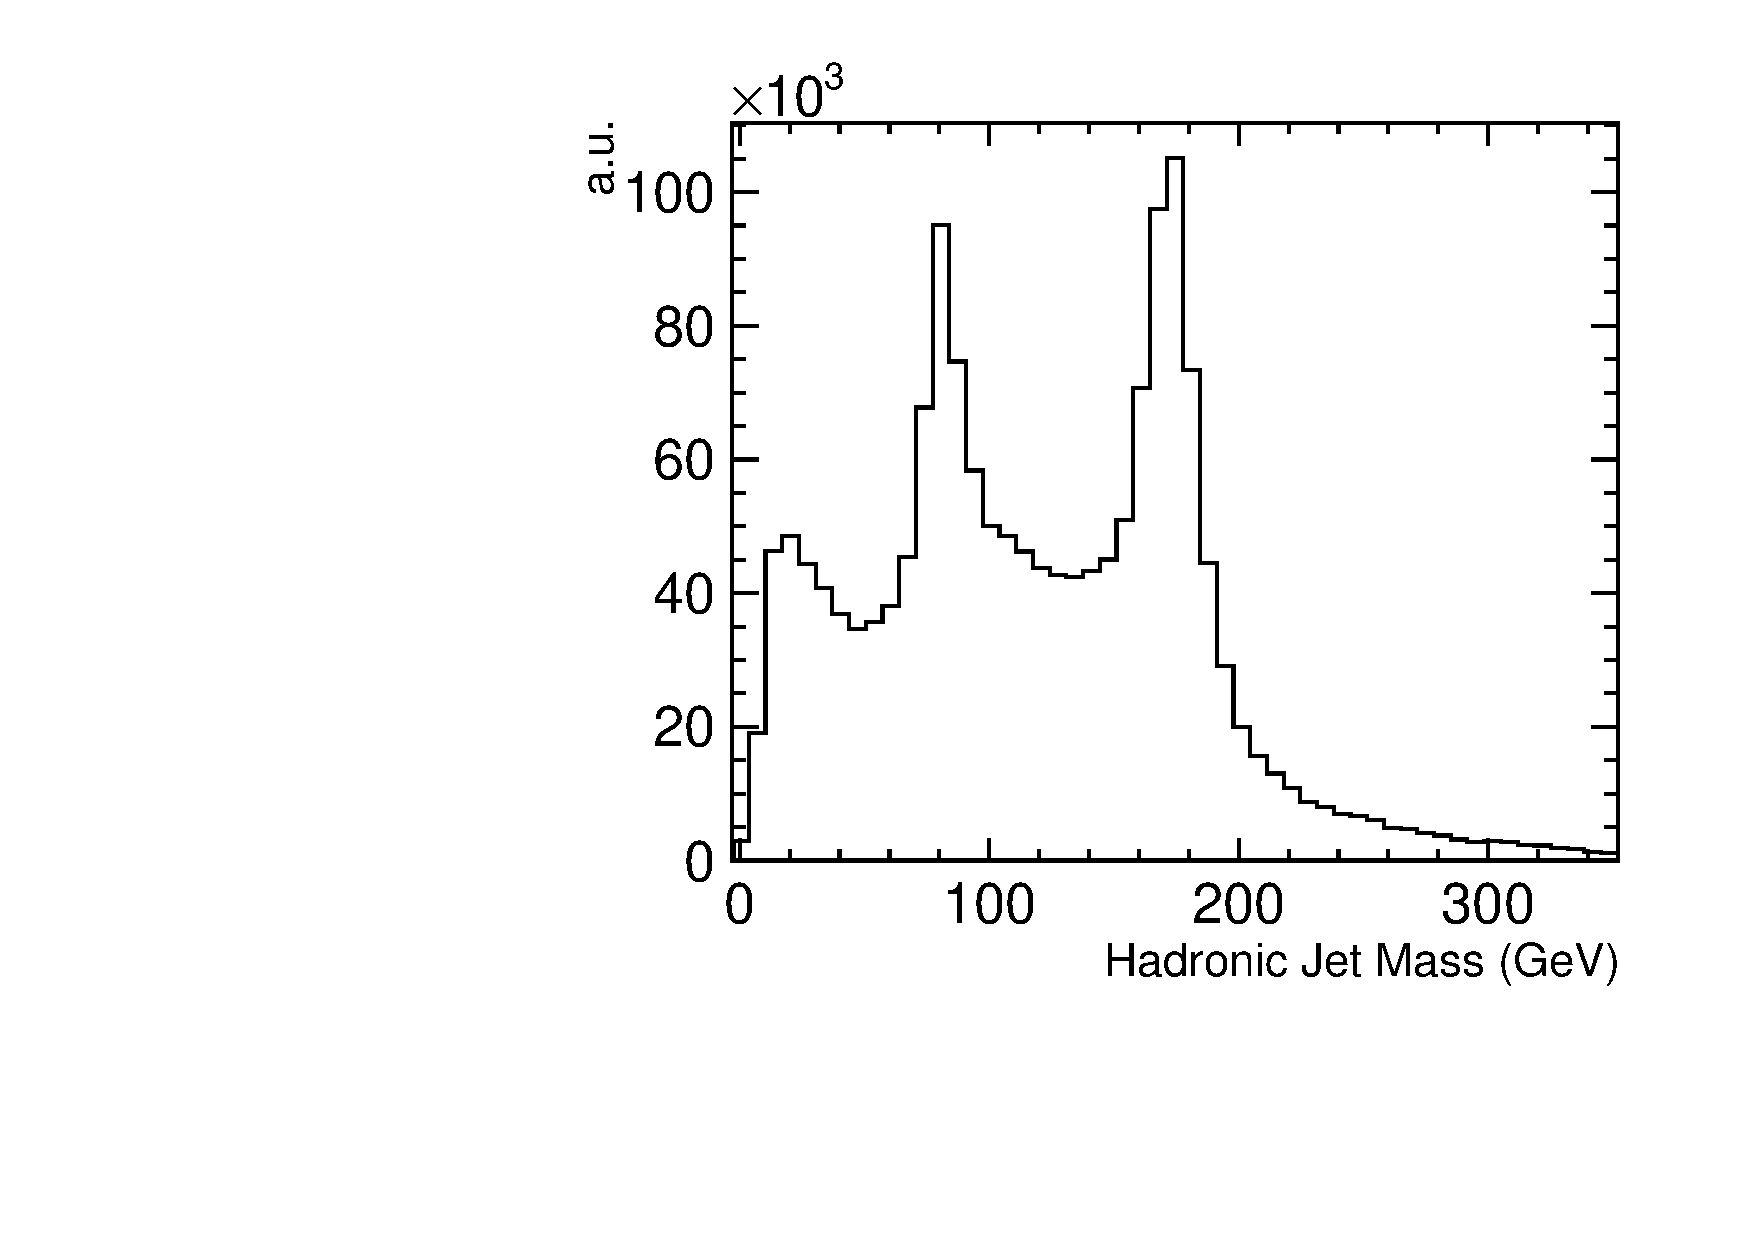
\includegraphics[width=1.0\textwidth]{TopAnalysis/figures/TopMassOffDiagonal.pdf}
 %   \caption[$\mid\frac{cos\theta_{Reco}}{cos\theta_{Generator}}\mid >1$]{Fat jet mass when $\mid\frac{cos\theta_{Reco}}{cos\theta_{Generator}}\mid <1$, off diagonal regions of fig \ref{fig:2djetangle}.}
  \end{subfigure}
  \caption[Reconstructed fat jet mass]{Reconstructed fat jet mass. Left: for the on diagonal elements of \reffig{fig:2djetangle}) where $\mid\frac{cos\theta_{Reco}}{cos\theta_{Gen.}}\mid >1$, the reconstructed fat jet matches the top mass. Right: in the regions corresponding to the off diagonal elements, the mass is no longer consistent.}
  \label{fig:diagonalTopMass}
\end{figure}


After the fat jet finding has been performed, the two reconstructed jets must then be associated as either coming from the hadronically decaying top or from the b jet from the leptonically decaying top. The default method for this was to associate the highest energy fat jet to the hadronically decaying top, as due to the neutrino not being reconstructed and the lepton already being removed, the remaining decay products from the leptonically decaying top should typically have considerably less energy. The performance of this method can be examined by comparing the reconstructed decay angle relative to the generator value (see \reffig{fig:2djetangle}). While the performance over most of the range studied is satisfactory, for $\mid \cos\theta \mid>0.9$ the correlation between the generator and reconstructed angles breaks down and off diagonal elements start to appear. Performance in these forward regions is typically poor due to the finite detector acceptance which results in losses down the beam line. In cases where parts of the hadronic top decay are not able to be reconstructed, using the fat jets energy to perform the jet association no longer becomes a reliable method. Evidence that misreconstruction is the source of these off diagonal elements is presented in \reffig{fig:diagonalTopMass} where it is clear that the fat jets in the off diagonal regions are not reconstructed with a consistent mass. If the jets are not fully reconstructed, it is more likely that the wrong jet is assigned to be from the hadronic top. When the wrong jet is selected the reconstructed angle will differ by approximately $\pi$ radians from the generator value as the tops are predominantly produced back to back. This explanation is further supported by the results shown in \reffig{fig:2djetangle_farfromleptop} which show that the off diagonal elements can be removed when a cut is placed on the angle between the reconstructed top and the generator level b jet from the leptonic top decay indicating that these elements are definitely coming from the wrong jet being selected. As well as the $\pi$ radian flips from selecting the wrong jet, there are also additional off diagonal contributions seen which arise from poor reconstruction of the fat jets. This typically happens when the tops are not produced back to back due to \ac{ISR}/\ac{BS}. When this happens, during the fat jet reconstruction it is possible for contributions from both true fat jets to be mixed e.g instead of grouping the three jets from the hadronic top together, only two of them are grouped together and the third is grouped with the lone b jet from the leptonic top. When this mismatching happens the hadronic top is no longer fully reconstructed and so the angle measured for the top decay has limited correlation with the generator value. \reffig{fig:2djetangle_goodtopseparation} shows that these remaining off diagonal elements disappear when a cut is placed on the separation of the tops at truth level. 

\begin{figure}
  \centering
  \begin{subfigure}{.48\textwidth}
    \centering
    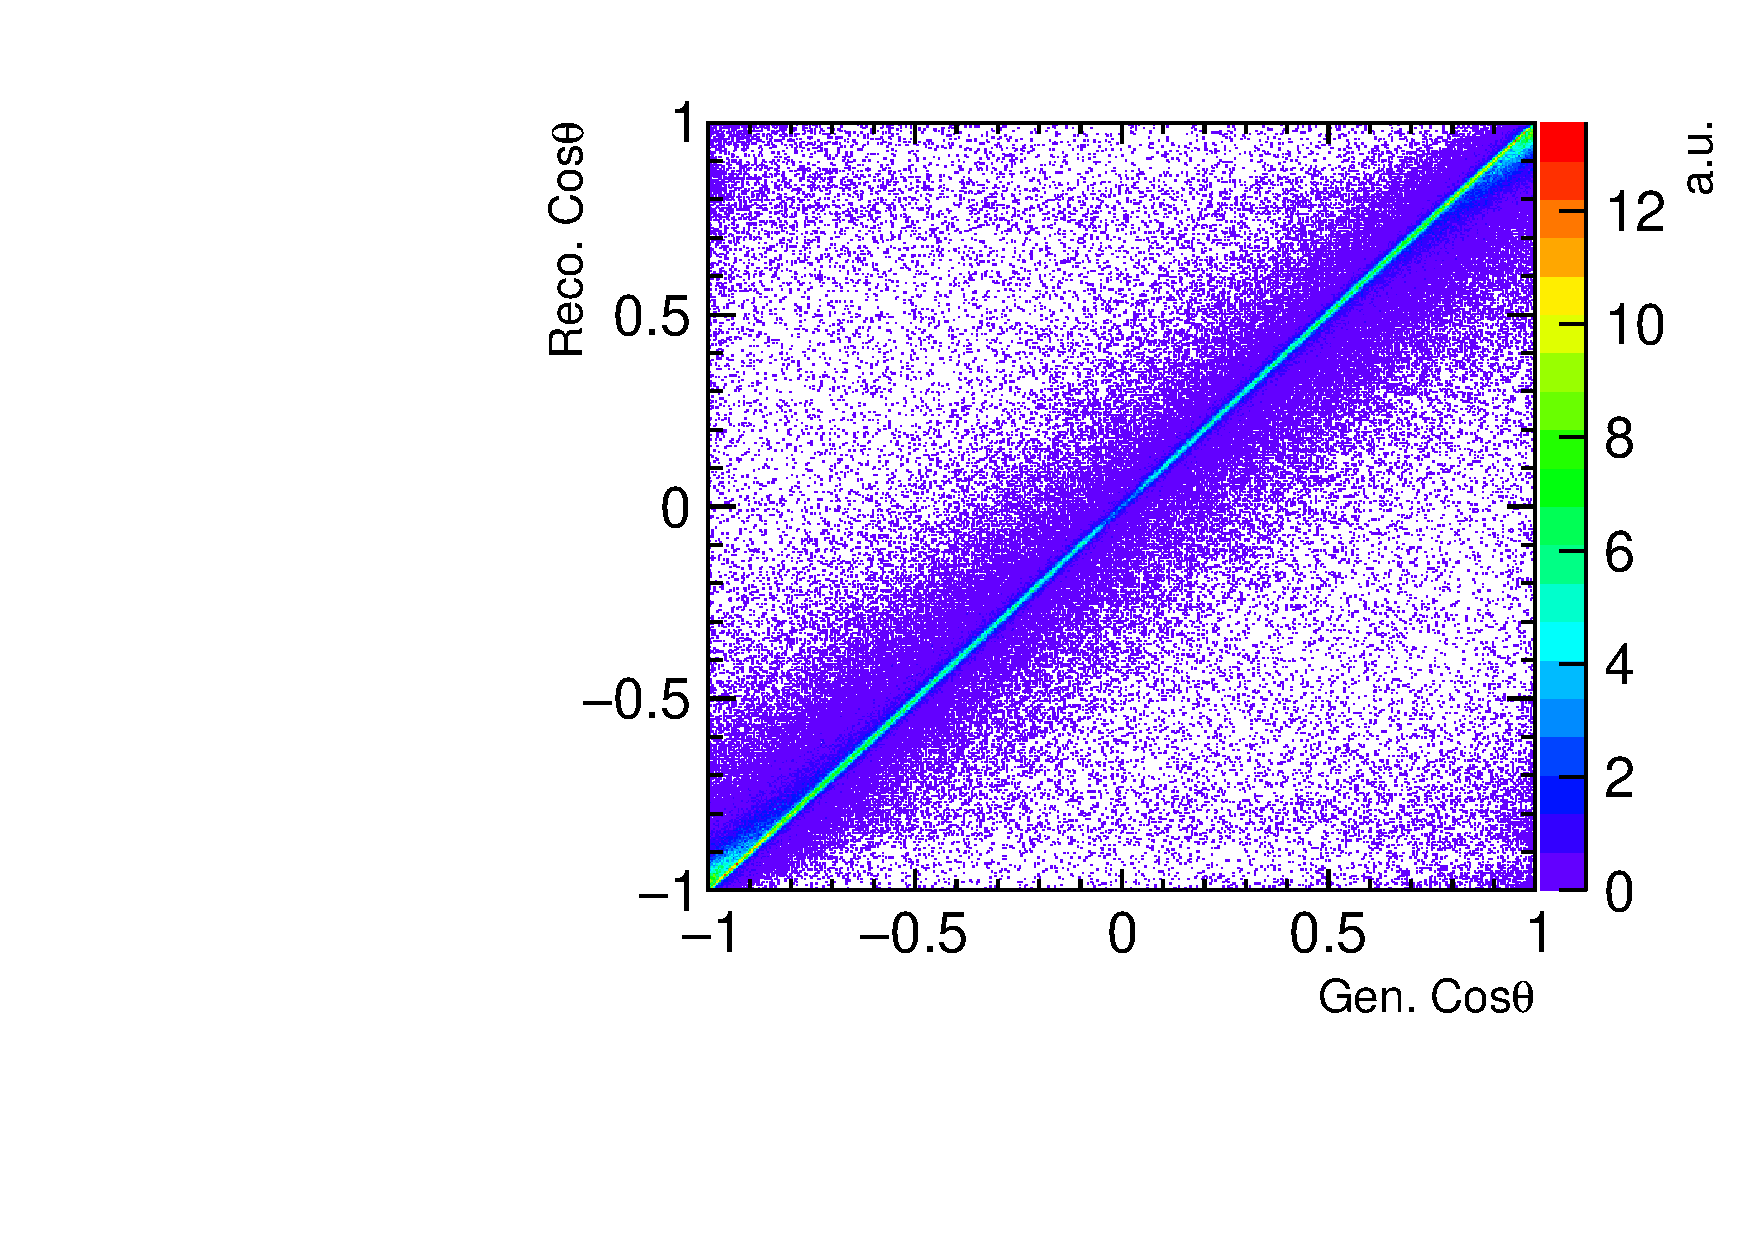
\includegraphics[width=1.0\textwidth]{TopAnalysis/figures/CosThetaRecoVsMC_NotNextToLepTop.pdf}%
    \caption[Cut placed on angle between reconstructed top and generator b jet from leptonic decay]{Cut placed on angle between reconstructed top and generator b jet from leptonic decay, $\Delta cos\theta_{Reco-Bjet}>0.1$.}
    \label{fig:2djetangle_farfromleptop}
  \end{subfigure}\hfill
  \begin{subfigure}{.48\textwidth}
    \centering
    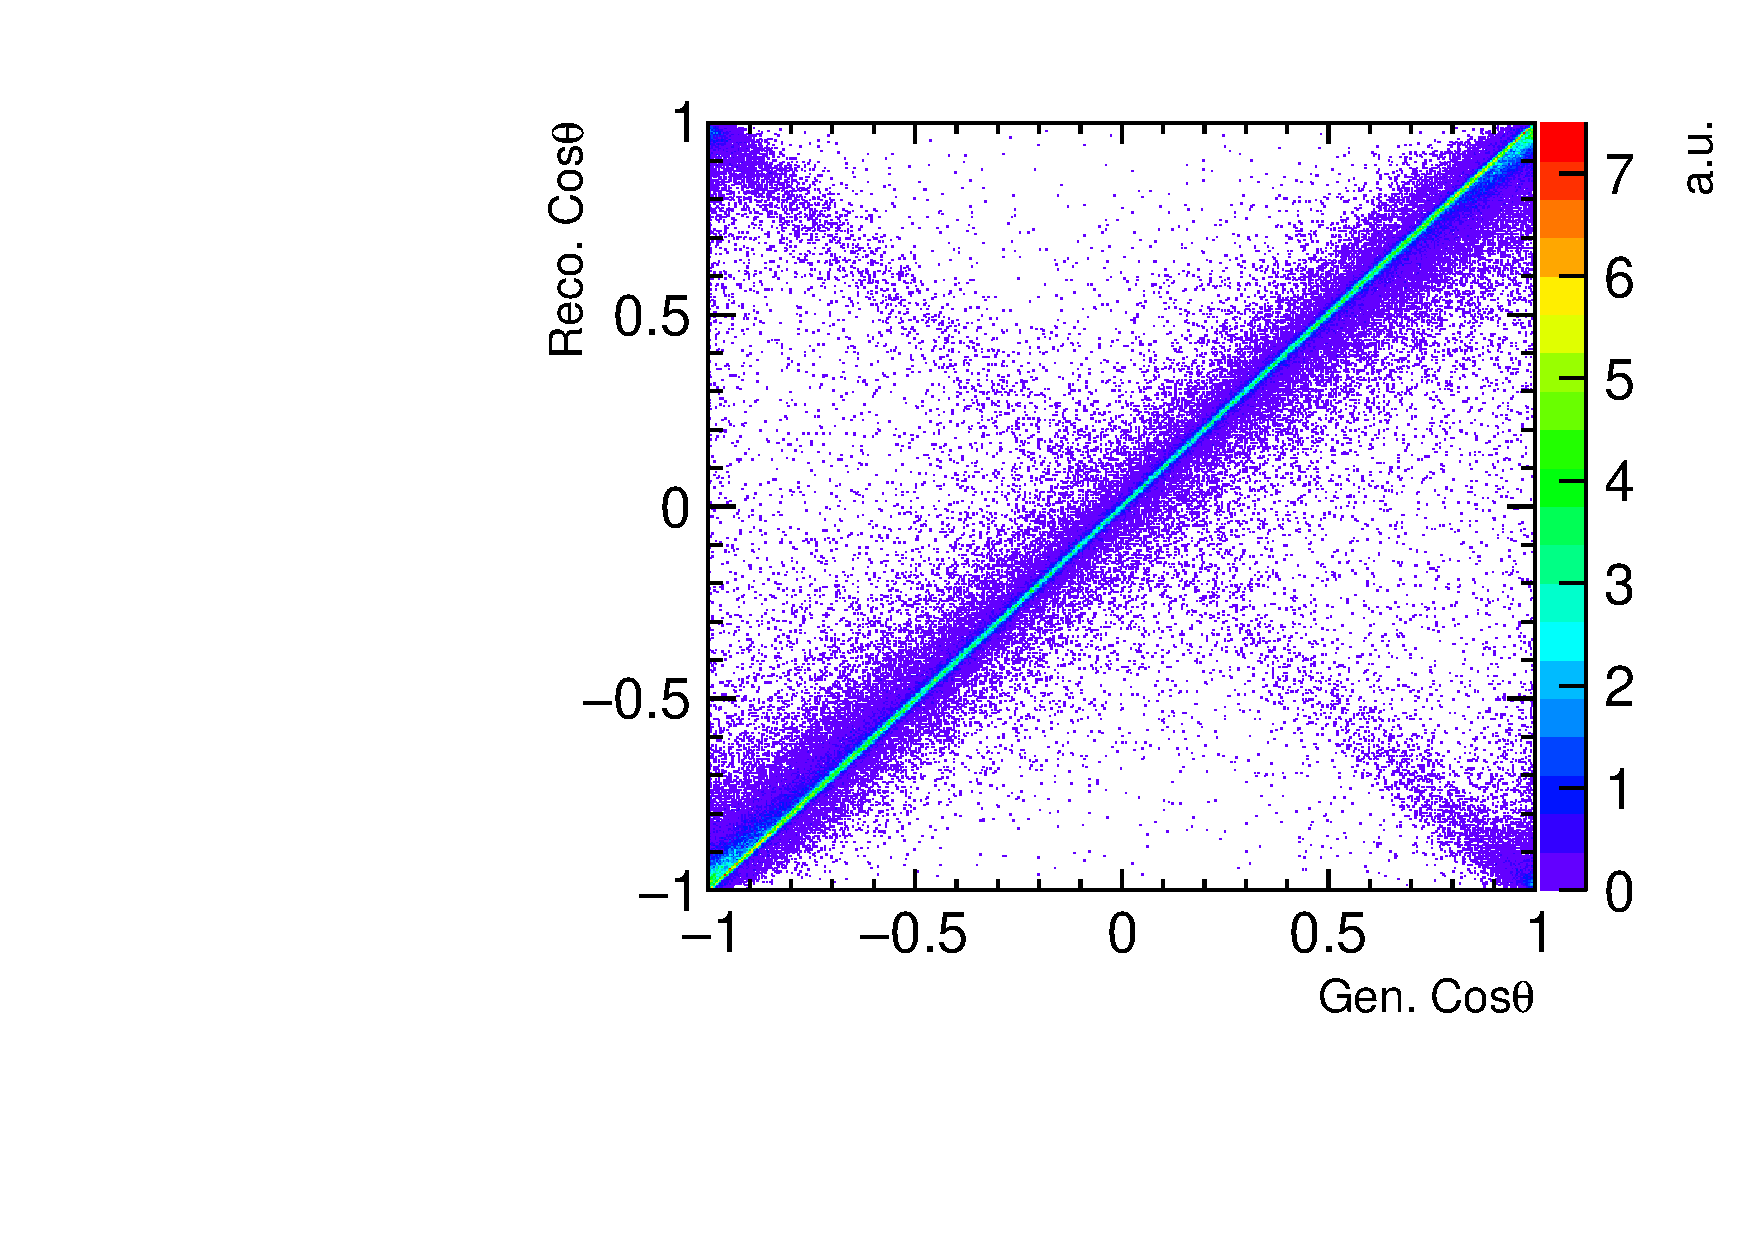
\includegraphics[width=1.0\textwidth]{TopAnalysis/figures/CosThetaRecoVsMC_MCTopsWellSeparated.pdf}%
    \caption[Cut placed on collinearity between top pair at generator level]{Cut placed on collinearity between top pair at generator level, separation $>$ 3 radians.}
    \label{fig:2djetangle_goodtopseparation}
  \end{subfigure}
  \caption[Reconstructed vs generator top decay angles with truth level cuts]{Reconstructed vs generator top decay angles with truth level cuts to explain the off diagonal elements seen in \ref{fig:2djetangle}.}
  \label{fig:2djetangle_explanations}
\end{figure}


In order to avoid the problems close to the beam line, multiple alternative jet association methods were devised- see \reftab{tab:methodDescription} for detailed descriptions.
\begin{table}
  \centering
  \begin{tabular}{l |p{100mm}}
    \toprule
    Fat Jet Selection Method     & Description  \\
    \midrule
    Lepton & The hadronically decaying top is deemed to be the fat jet with the greatest angular separation from the isolated lepton\\
    \midrule
    B tag & The hadronically decaying top is deemed to be the fat jet with the greatest angular separation from the jet with the highest b tag (see \ref{Flavour Tagging} for details on how flavour tagging is performed)\\
    \midrule
    Energy & Select the fat jet with the highest energy to be the hadronically decaying top\\
    \midrule
    Multiplicity & Recluster both fat jets into N ``micro jets'' (see \ref{Jet Multiplicity} for methodology.) The hadronically decaying top should have a higher number of micro jets found within it\\
    \midrule
    Mass & The hadronically decaying top is deemed to be the fat jet with the greatest mass \\
    \midrule
    Top Mass & Select the fat jet with mass closest to the nominal top mass as the hadronically decaying top \\
    \midrule
    Democratic & A combination of the lepton, energy and mass methods. Each method votes for which fat jet it thinks is the hadronically decaying top. The fat jet with the most votes is then selected as the hadronically decaying top  \\
    \bottomrule
  \end{tabular}
  \caption{Methods used for identifying which fat jet corresponds to the hadronically decaying top.}
  \label{tab:methodDescription}
\end{table}

The relative effectiveness of these methods were evaluated in three ways shown in \reffigs{fig:methodComparison}, \ref{fig:angleFitDiff} and \ref{fig:angularEfficiency} respectively. The first method was to look at the overall distribution of $cos\theta$ produced by each method compared to the distribution at generator level as this is what will be used to extract $A_{FB}^{t}$. All the methods agree well with the generator distribution in the central region of the detector but diverge in the high $\mid\cos\theta\mid$ region. This is mainly caused by the effects described above. Close to the beam line the jets are not fully reconstructed, the jet association fails and the b jet from the leptonic side is selected rather than the hadronic top jet. This causes migrations from the forward region to the backward regions producing a deficit in the forward region and an excess in the backward region. Migrations do occur in the opposite direction too for the same reason, however because the top forward-backward asymmetry means that more tops are produced in the forward region to begin with, the net migration is from forward to backward. The migrations are not always a shift of $\pi$ radians as one might expect. Instead the migrations occur from very close to the beam line to a broader range in the opposite direction. This is due to the fact that \ac{ISR}/\ac{BS} can mean the top pair are not produced exactly back to back in the lab frame and because the b-jet produced by the leptonic decay is not exactly collinear with the top decay axis. Comparing the methods we see that they all show similar levels of migration except for the btag method which shows the highest migration. This is attributed to the fact the highest btagged jet can sometimes be from the hadronic side even in events that are well reconstructed, and so the jet association will fail in more events than the other methods which only fail for events close to the beam line.

\begin{figure}
  \centering
  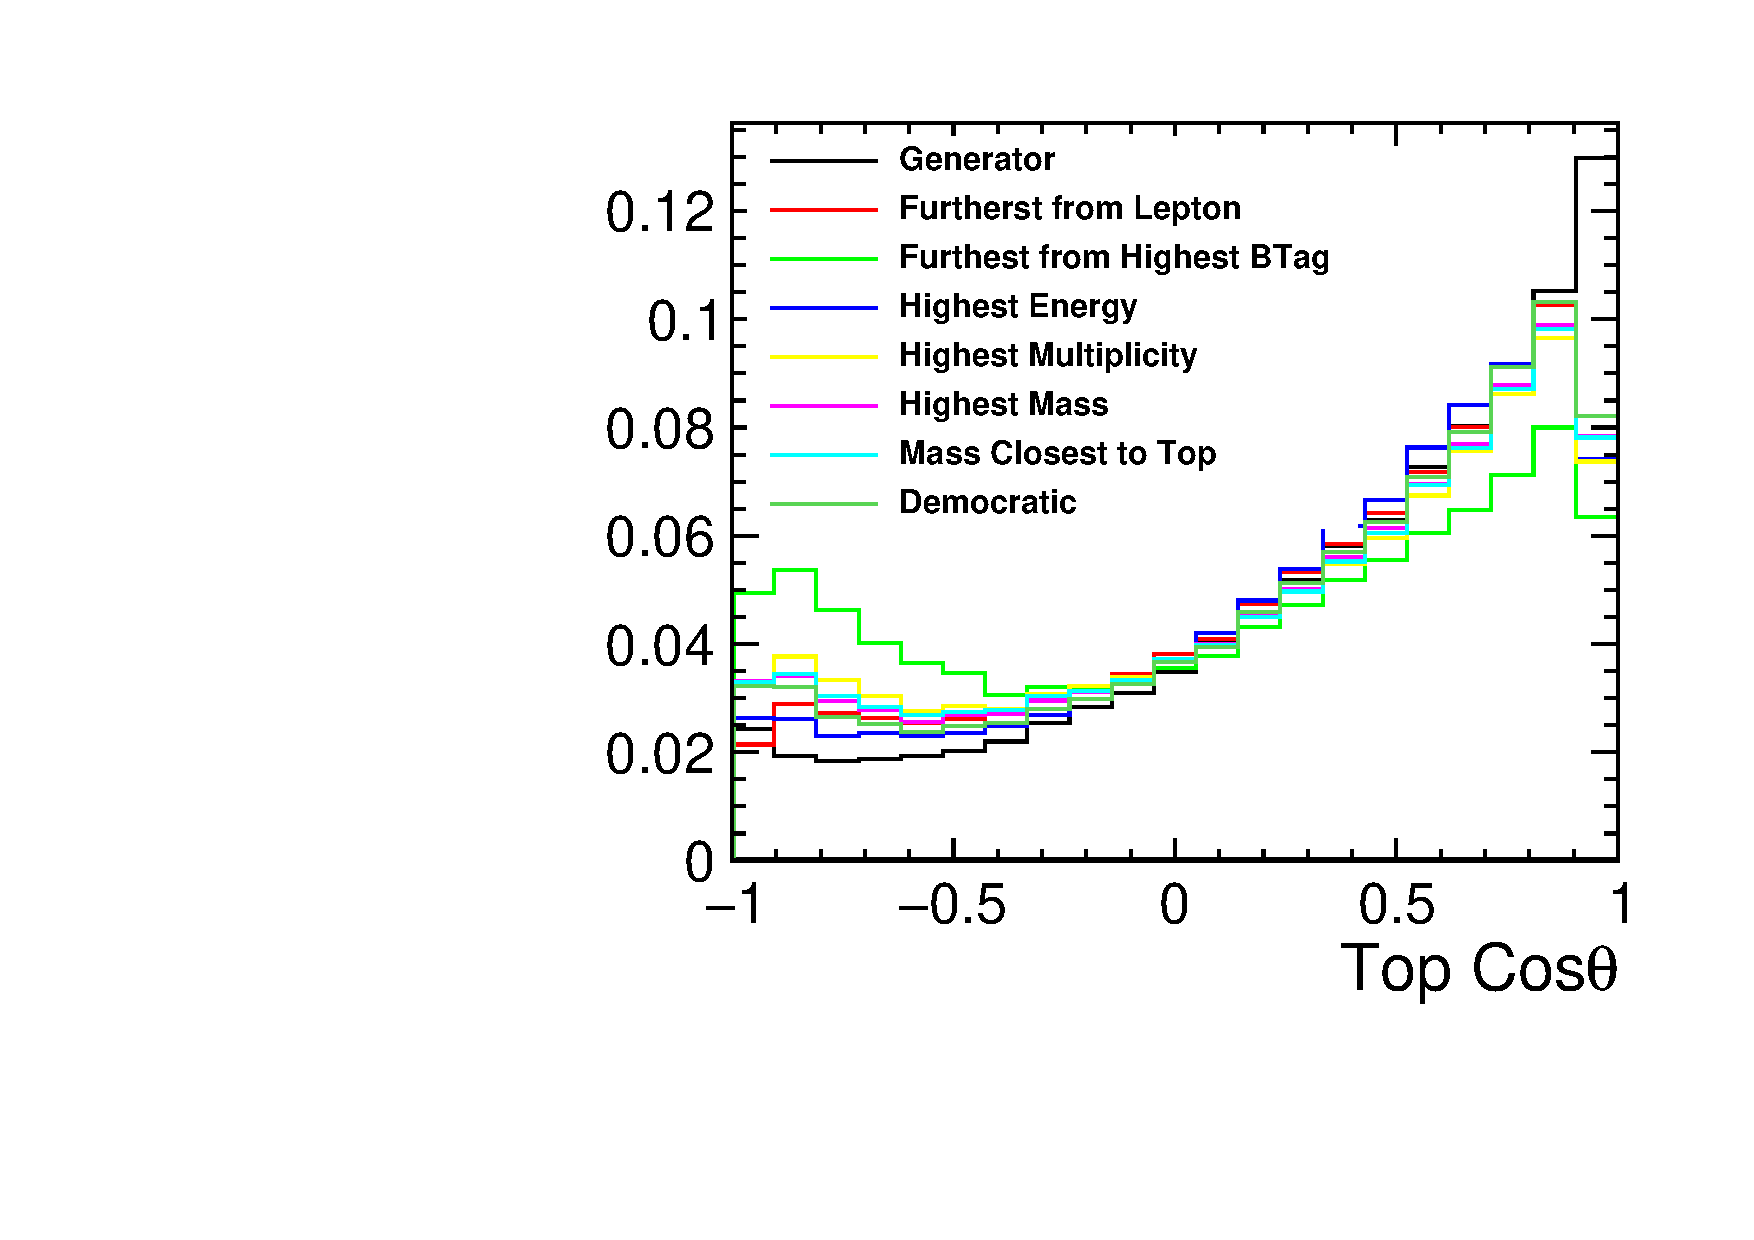
\includegraphics[width=0.8\textwidth]{TopAnalysis/figures/comparejetmethods.pdf}
  \caption[Reconstructed $cos\theta$ distribution for various jet association methods]{Reconstructed $cos\theta$ distribution for various jet association methods. The expected distribution from truth level information is included for reference.}
  \label{fig:methodComparison}
\end{figure}

The second method was to measure the difference between the reconstructed and MC(generator) $cos\theta$ per event and fit this with a Gaussian function. The variation in the width and mean of these distributions were plotted against the generator $cos\theta$ and are shown in \reffig{fig:angleFitDiff}. The effects of migration at high $cos\theta$ is more pronounced in these plots where in the width we can see that the resolution on $cos\theta$ gets much worse in the forward regions and the mean shows a pull in opposite directions in these regions proving the migrations do indeed occur in both directions with the same rate. Unfortunately there is little discrimination seen between the methods except for showing that there are slightly larger migrations when using the b-tag method.

\begin{figure}
  \centering
  \begin{subfigure}{.8\textwidth}
    \centering
    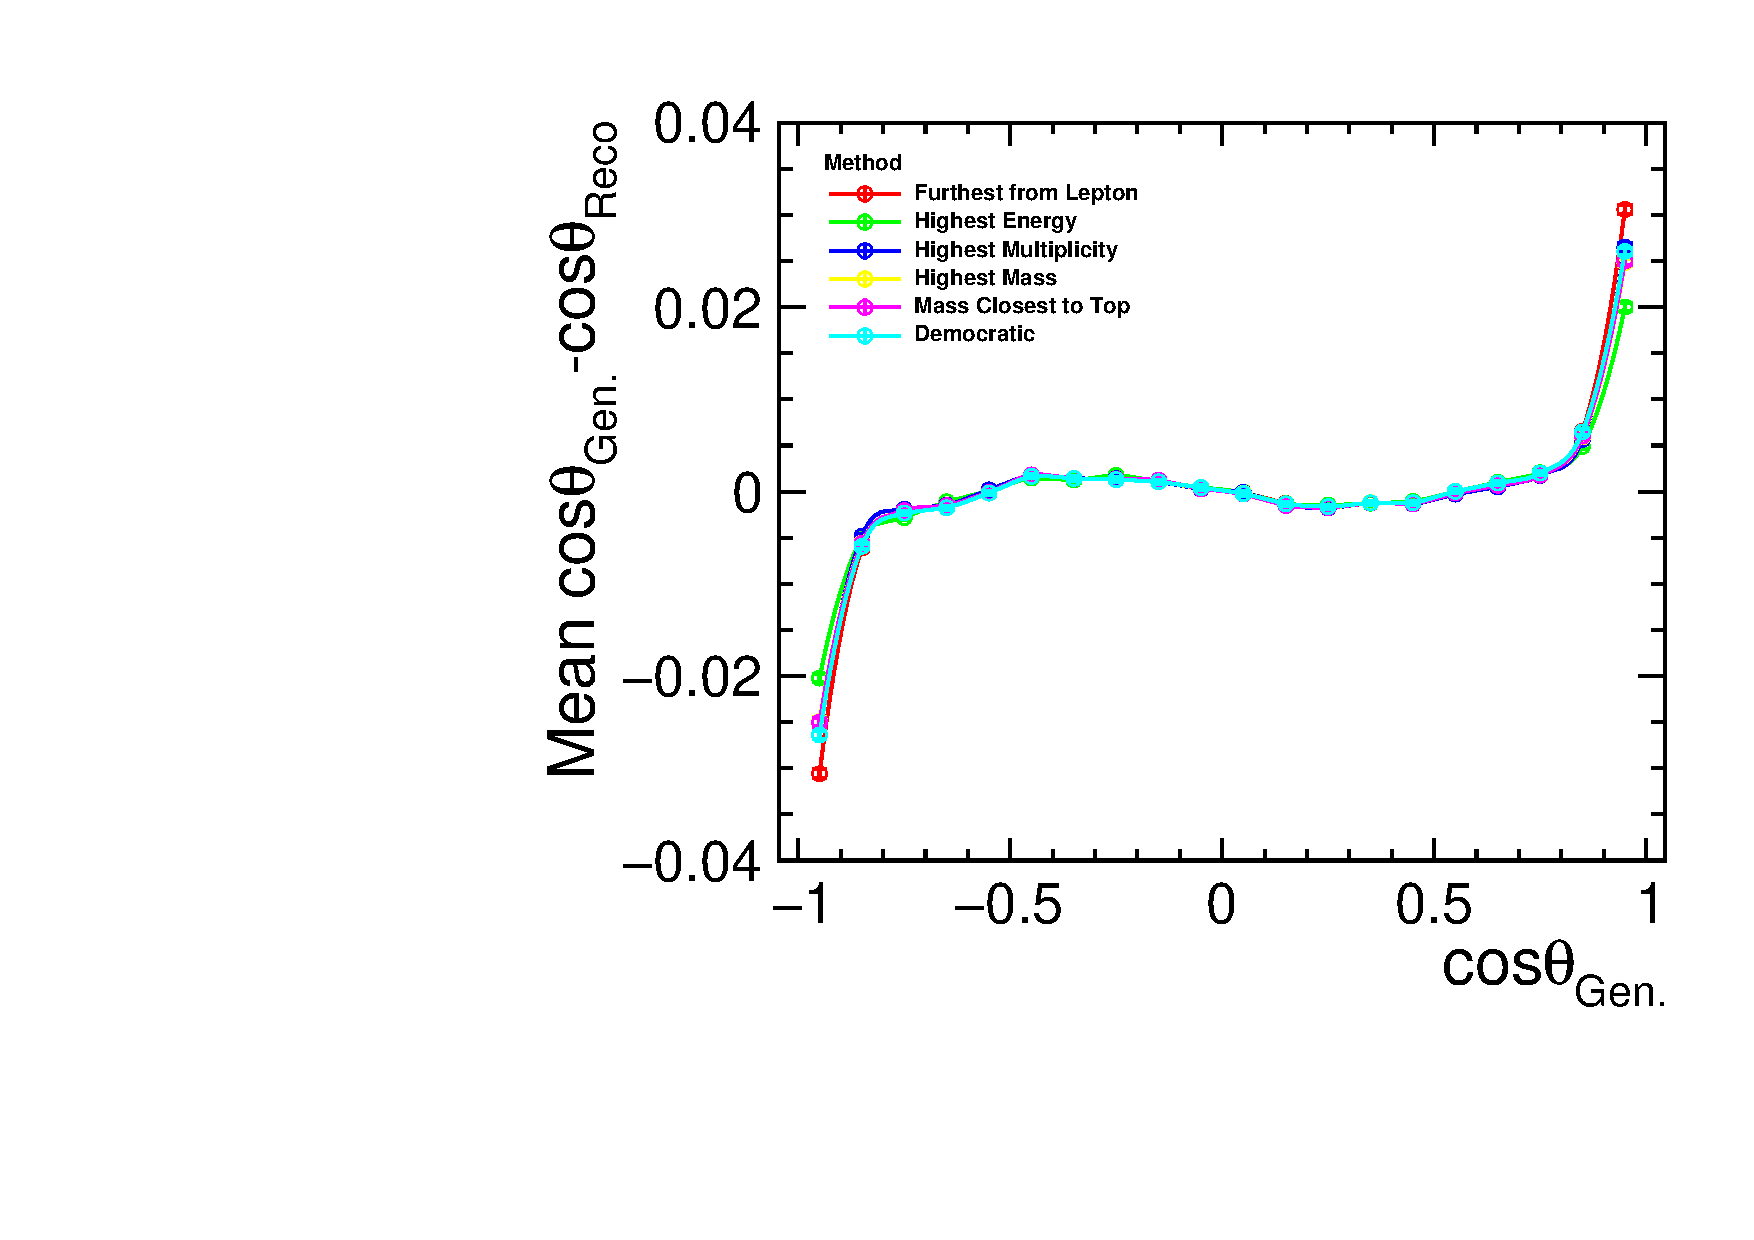
\includegraphics[width=0.99\textwidth]{TopAnalysis/figures/MeanThetaDiff.pdf}
    \caption[Mean]{Mean}
  \end{subfigure}
  \begin{subfigure}{.8\textwidth}
    \centering
    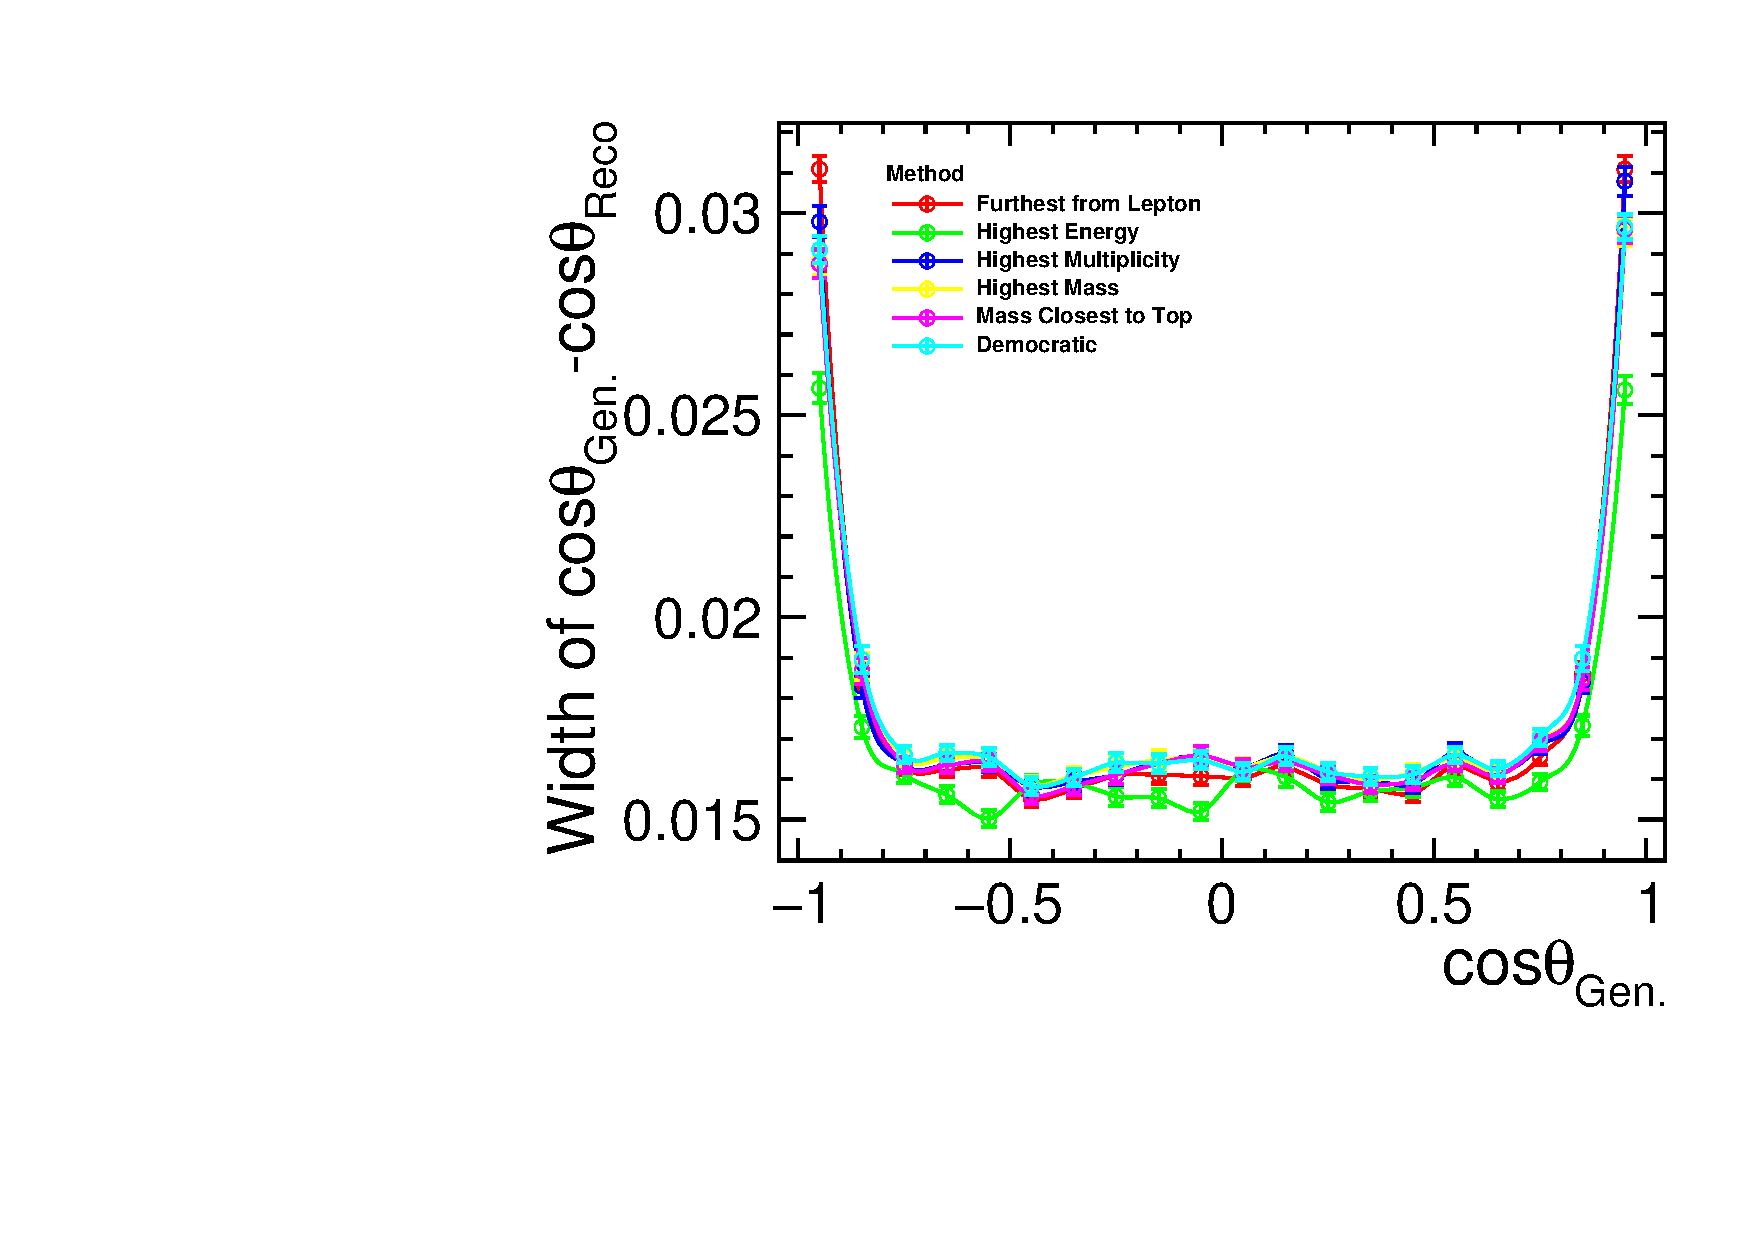
\includegraphics[width=0.99\textwidth]{TopAnalysis/figures/WidthThetaDiff.pdf}
    \caption[Width]{Width}
  \end{subfigure}
  \caption[Mean and width from fitting $\Delta cos\theta_{Gen.-Reco.}$ to a Gaussian]{Mean and width from fitting $\Delta cos\theta_{Gen.-Reco.}$ to a Gaussian. Mean: migrations close to $\mid cos\theta\mid>0.9$ result in a bias in the mean. The migrations cause a shift of roughly $\pi$ radians resulting in the bias being in the opposite direction for each end of the range. Width: migrations close to $\mid cos\theta\mid>0.9$ cause a broadening in the resolution of the reconstructed $cos\theta$.}
  \label{fig:angleFitDiff}
\end{figure}

The final method of comparison was to measure the efficiency with which the hadronic top was measured within the correct $cos\theta$ bin as a function of the generator $cos\theta$. For this study a bin width of 0.1 in $cos\theta$ was used. The results are shown in \reffig{fig:angularEfficiency}. Here there is a clearer separation in the performance of the different methods. B-tagging is seen to provide the worst efficiency while the energy and democratic methods provide the highest level of performance. The mass based selections provide slightly lower performance than the energy/democratic methods. This is likely to be explained by the fact they are less robust when the jets are not fully reconstructed. Missing a small section of the jet via acceptance losses/reconstruction inefficiencies can have a large impact on the reconstructed mass, however in the case of energy, if we naively assume that the energy is split evenly between the six final state particles, then we would expect that the energy of the hadronic fat jet would be three times that of the b-jet from the leptonic top and so considerable energy losses must occur before the wrong jet is selected. Due to its higher bin by bin efficiency, the energy method is chosen as the preferred method for the rest of the analysis. 

\begin{figure}
  \centering
  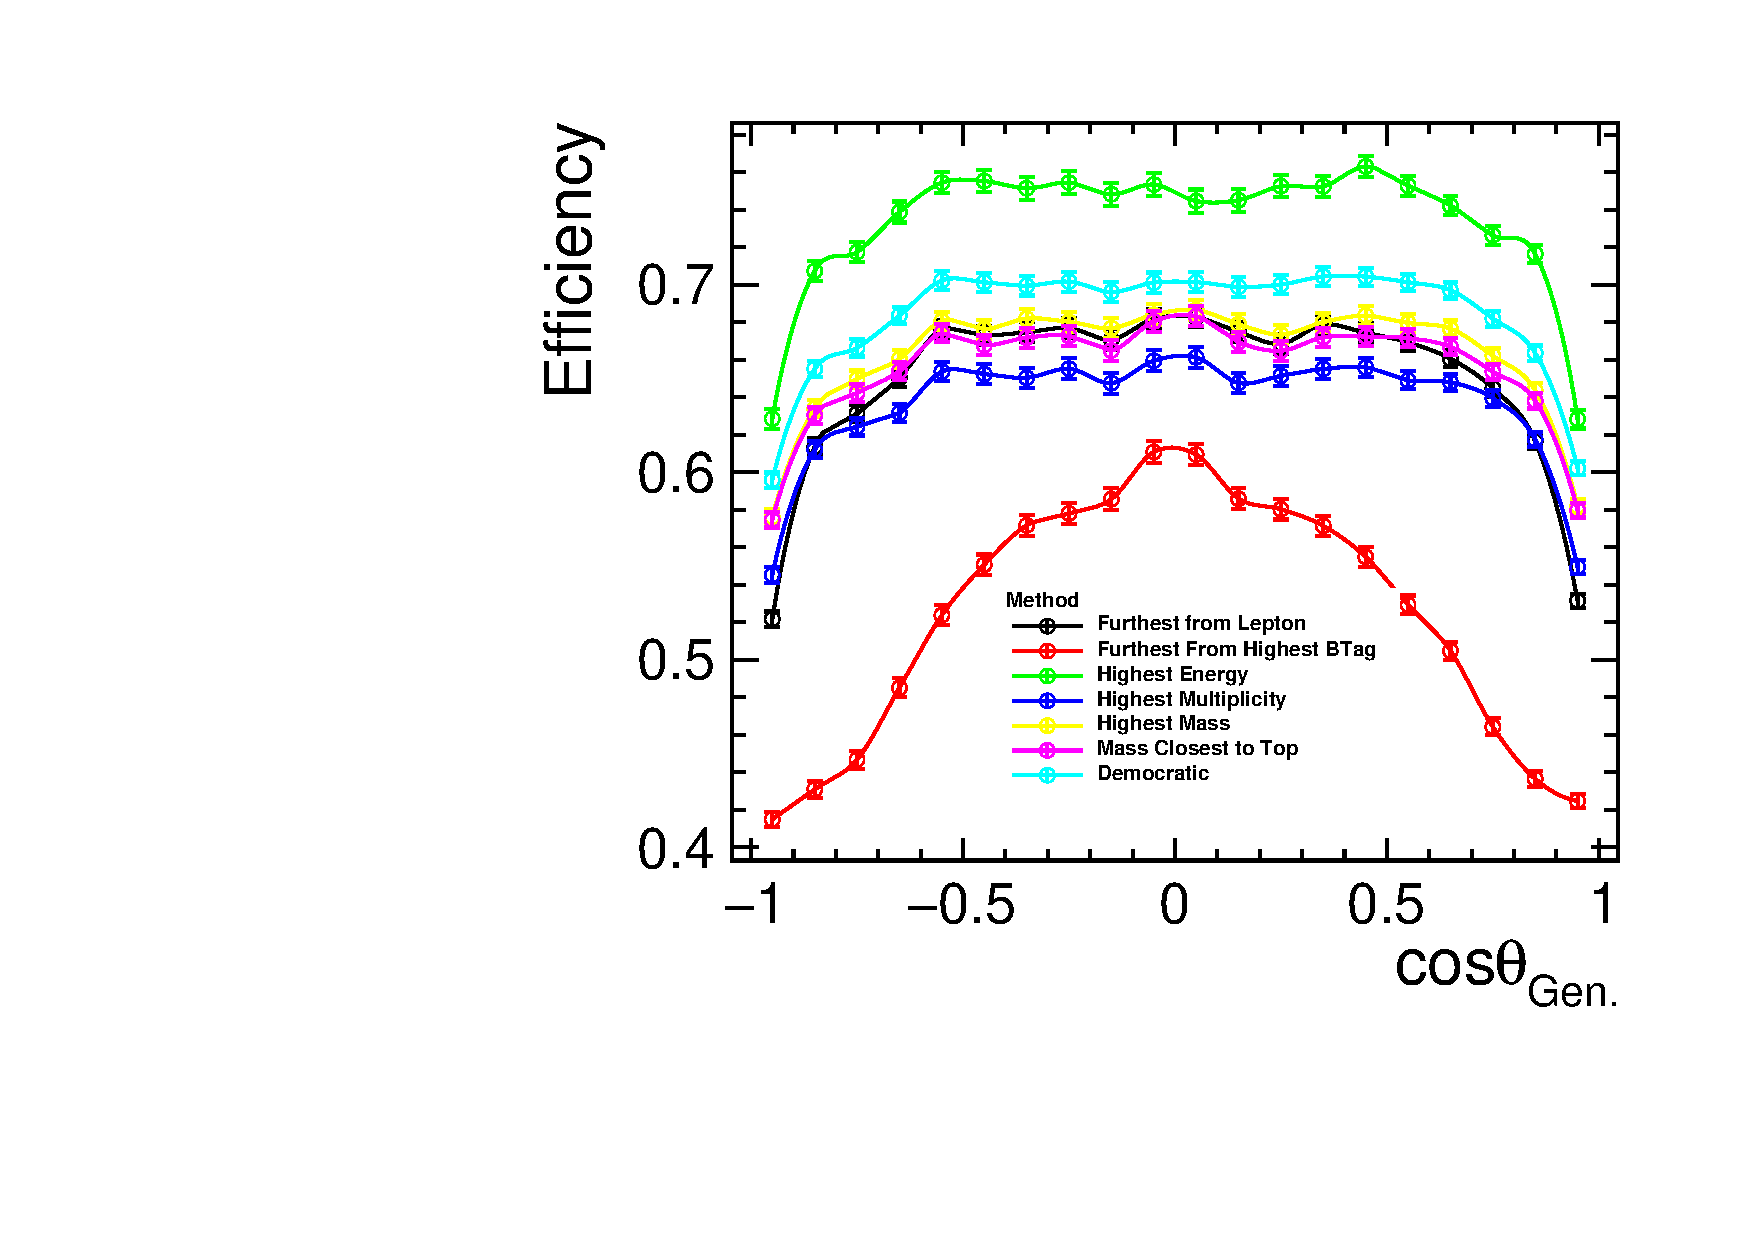
\includegraphics[width=0.8\textwidth]{TopAnalysis/figures/EfficiencyvsMCTheta.pdf}
  \caption[Efficiency for reconstructing the hadronically decaying top in the correct cos$\theta$ bin]{Efficiency for reconstructing the hadronically decaying top in the correct cos$\theta$ bin.}
  \label{fig:angularEfficiency}
\end{figure}

\subsection{Jet Substructure}
After the fat jets have been found, in order to help distinguish signal events from similar background, it is useful to look at the substructure of these jets. To do this, three substructure variables were considered.

\subsubsection{N-subjettiness}
N-subjettiness is a substructure variable that is already being used in experiments at the LHC and is used to measure how many subjets are present within a fat jet. In the signal channel one would expect the hadronic fat jet to contain three subjets (one b quark and two light quarks from the W decay) and the leptonic fat jet to have only one subjet. In order to calculate the N-subjettiness, each fat jet is reclustered into N subjets. For this analysis this was done using the kt algorithm, R=0.3. After reclustering, the N-subjettiness is then defined as\cite{Thaler:2010tr}:

\begin{equation}
  \label{eq:nsubjet}
  \tau_N=\frac{1}{d_0}\sum\limits_{k}p_{T,k}~\text{min}\{\Delta R_{j_1,k},\Delta R_{j_2,k},.....,\Delta R_{j_N,k},\},
\end{equation}

where $k$ labels the constituent particles of the fat jet, j$_{i}$ label the subjets, $\Delta R$ is the distance in the rapidity-azimuthal plane, p$_{T}$ is transverse momentum and d$_0$ is a normalization parameter typically taken to be

\begin{equation}
  d_0=\sum\limits_{k}p_{T,k}R_0
\end{equation}

Where R$_0$ is the jet radius used when reclustering the fat jet into the N subjets. One can see from \refeq{eq:nsubjet} that N-subjettiness is simply the sum of the angular separation between each particle in the fatjet and its nearest subjet axis weighted by the transverse of momentum of the particle. In the case that too few subjets have been chosen, the separation between the particles and the subjet axis will be large and so $\tau_N$ will be large. If instead the correct number of subjets are chosen, then all the particles are close to a subjet axis and $\tau_N$ will be closer to zero. This is perhaps more easily understood diagrammatically in \reffig{fig:nsubjet}.

\begin{figure}
  \centering
  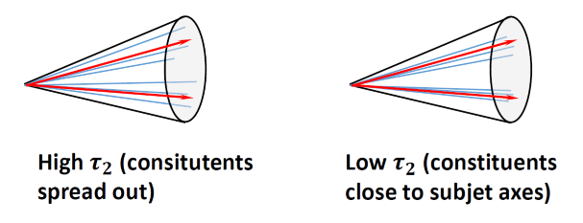
\includegraphics[width=0.9\textwidth]{TopAnalysis/figures/nsubjettiness.png}
  \caption[Diagrammatic representation of N-subjettiness]{Diagrammatic representation of N-subjettiness.}
  \label{fig:nsubjet}
\end{figure}

While the magnitude of $\tau_N$ does measure the substructure of the subjet, it is not possible to use it by itself to determine the correct number of subjets within a fatjet. This comes from the fact that while selecting too few subjets results in a higher value of $\tau$, selecting too many jets actually results in a lower value of $\tau$ and so there is no minimum $\tau_N$ that decides the true number of subjets. As an example, take the case shown on the right hand side of \reffig{fig:nsubjet}. For two subjets, the value of $\tau_2$ is clearly going to be quite small as the particles are all aligned along the two subjet axes. However, if the fat jet was instead reclustered into three subjets, the most likely outcome would be that one of the two existing subjets would be artificially split into two new subjets. The two new subjet axes for the artificially split subjet would both be placed within the ``true'' subjet and so when calculating the angular separation between the particles of the true subjet and the new axes, the distance will be smaller than in the original case as there are now more axis to choose from. As a result $\tau_3$ will be lower than $\tau_2$. This logic is true for any number of subjets and so it is almost always true that $\tau_N > \tau_{N+1}$. It is also not possible to simply place a cut on a specific $\tau_N$ as the absolute value of $\tau_N$ can depend on how diffuse the jets are. Again this is best seen from \reffig{fig:nsubjet}. By inspection it is clear that the left hand event is a diffuse single subjet event while the right hand event is a two subjet event, however if one were to calculate $\tau_1$ for both events the right hand event would have the lower $\tau_1$ as the two subjets are relatively close to each other and so none of the particles would be particularly far from their combined central axis, while in the single subjet event, all of the particles are spread out and so the angular separation relative to a central axis would be larger.

In practice it turns out that the easiest way to get around these issues is to look at the ratio of $\tau_{N+1}/\tau_N$ rather than just $\tau_N$. This metric instead shows the improvement in $\tau_N$ from increasing the number of subjets. For a jet with three true subjets one expects a small value for $\tau_{3}/\tau_2$ and $\tau_{2}/\tau_1$ as the angular separations are being less limited by the lack of sufficient jet axes. For $\tau_{4}/\tau_3$ and above the value should be much closer to one because at this point any new jet axes will be the result of an artificial jet splitting and so the new axis will typically be very close to one of the old axes and so provides little improvement in the angular separation of the particles to their nearest axis.

An example of one of the N-subjettiness variables used here is the ratio $\tau_{2}/\tau_1$ for the leptonic fat jet (see \reffig{fig:lepfatjetsubjet}). For signal events where the expected number of subjets is one, the effect of adding an additional subjet axis is minimal and so the ratio is close to one. For many of the background e.g. qqqq, there will be two subjets within the fat jet and so the difference between $\tau_{2}$ and $\tau_1$ is more significant.

\begin{figure}
  \centering
  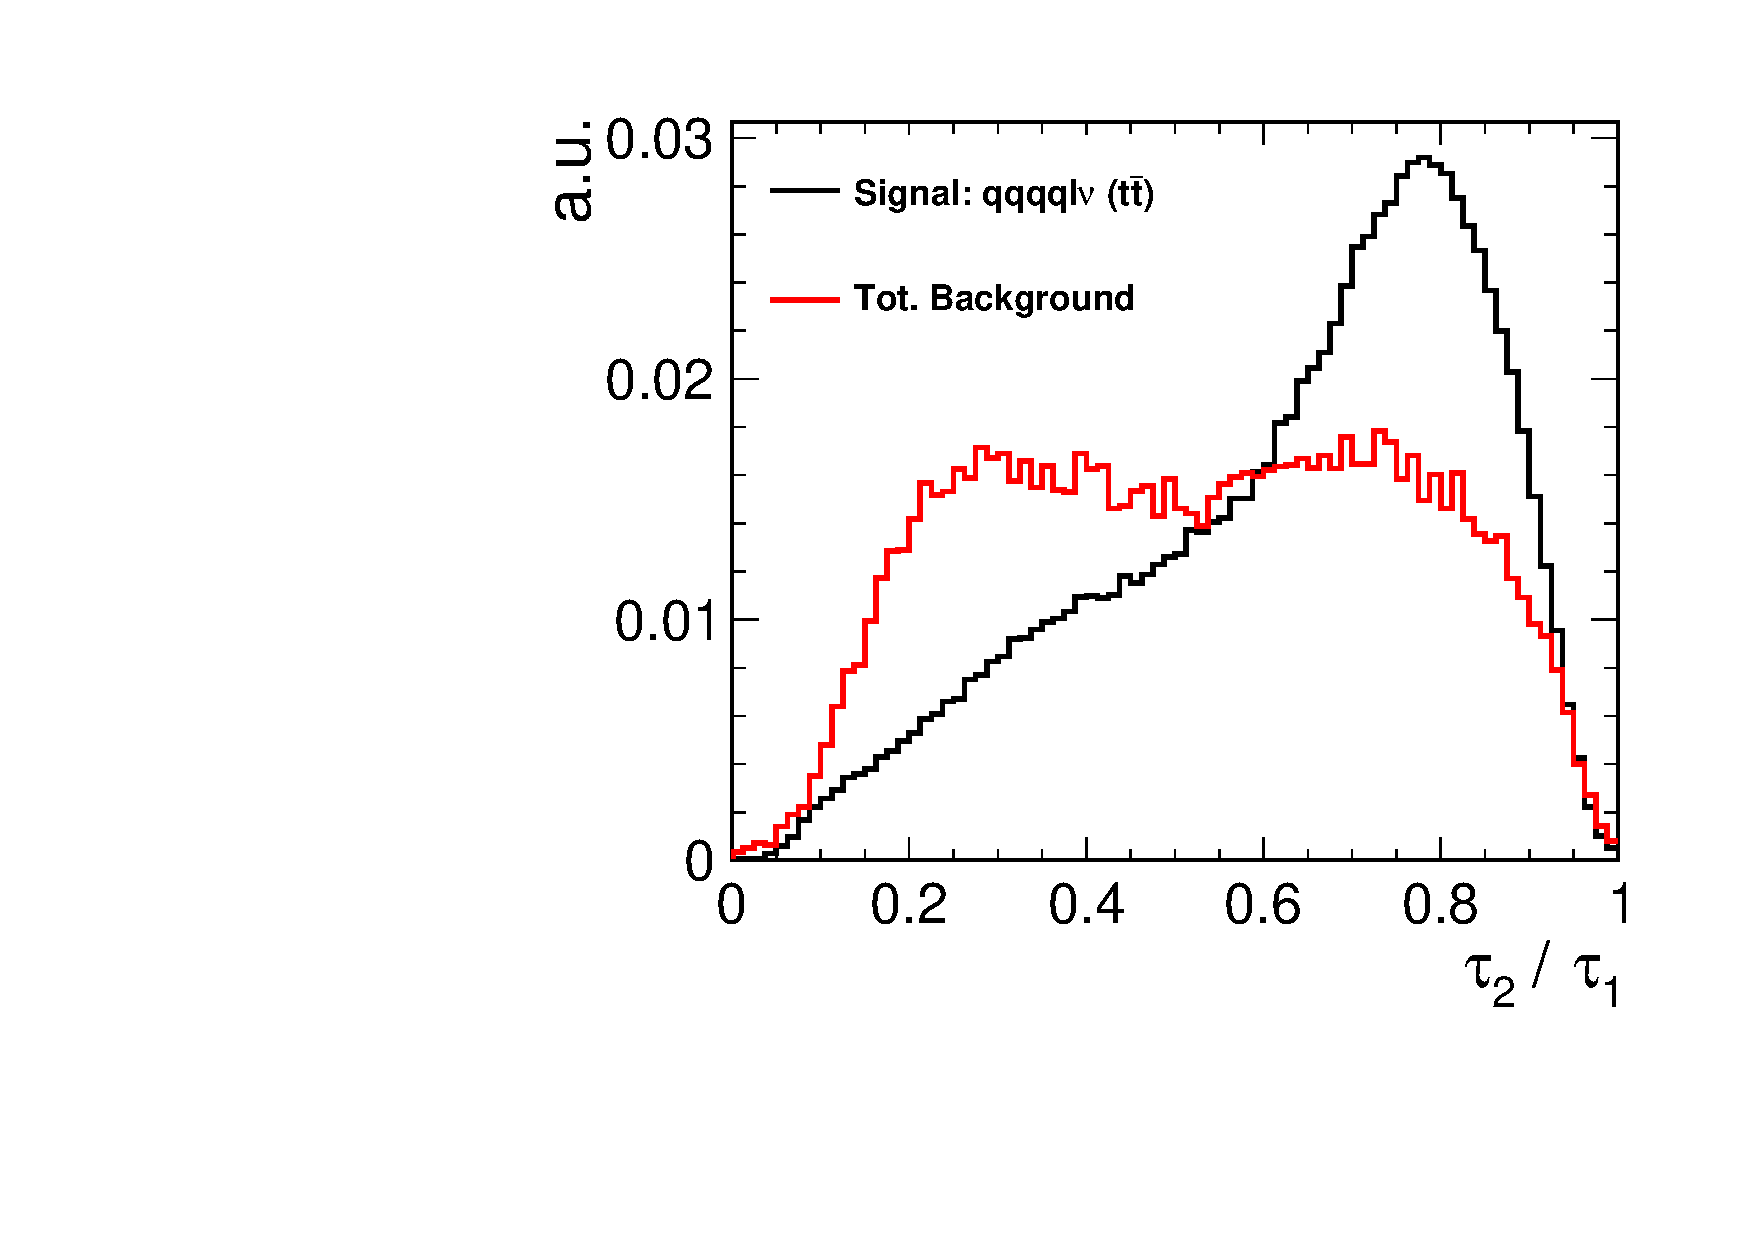
\includegraphics[width=0.6\textwidth]{TopAnalysis/figures/NSubJettiness.pdf}
  \caption[Ratio of $\tau_{2}$ to $\tau_1$ for the leptonic fat jet for both signal and background processes]{Ratio of $\tau_{2}$ to $\tau_1$ for the leptonic fat jet for both signal and background processes.}
  \label{fig:lepfatjetsubjet}
\end{figure}

  
\subsubsection{Subjet Angular Distributions}
\label{subjAngular}
\begin{figure}
  \centering
  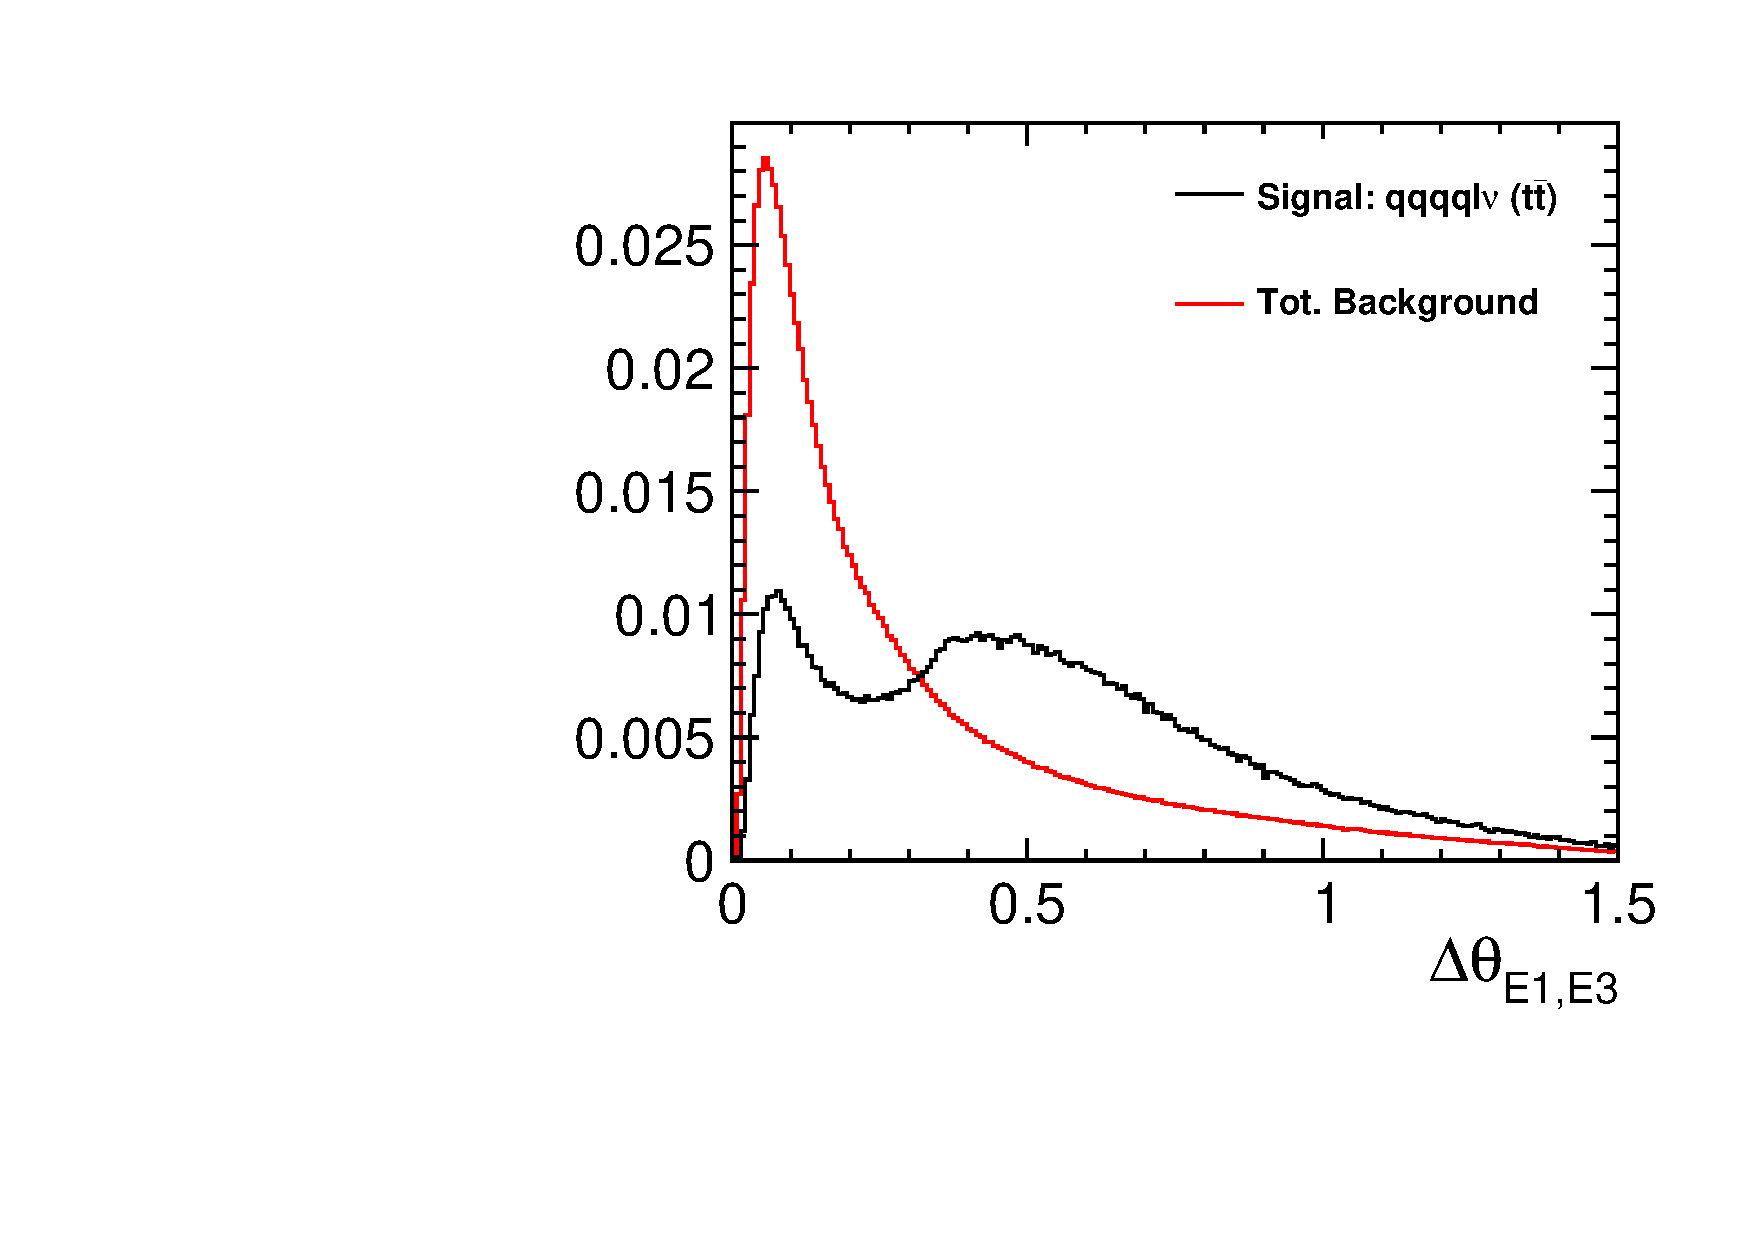
\includegraphics[width=0.8\textwidth]{TopAnalysis/figures/HighELowEDira.pdf}
  \caption[Angular separation of highest and lowest energy subjets]{Angular separation of highest and lowest energy subjets}
  \label{fig:angularrelations}
\end{figure}


As already described above, in the case that a fat jet is reclustered into more subjets than it should be, the subjets arising from the artificial splitting of a ``true'' subjet will typically be produced with minimal separation between them. This can be exploited to identify background events with a lower number of subjets than are present in the signal events. This is achieved by reclustering the hadronic fat jet into three subjets using the kt algorithm, R=0.3. The three resulting subjets are then ordered by energy and the angular separation between each of the them is determined. For background events the angle between these subjets is expected to be considerably smaller. The angular separation between the highest and lowest energy subjets is shown in \reffig{fig:angularrelations}.



\subsubsection{Jet Multiplicity}
\label{Jet Multiplicity}

\begin{figure}
  \centering
  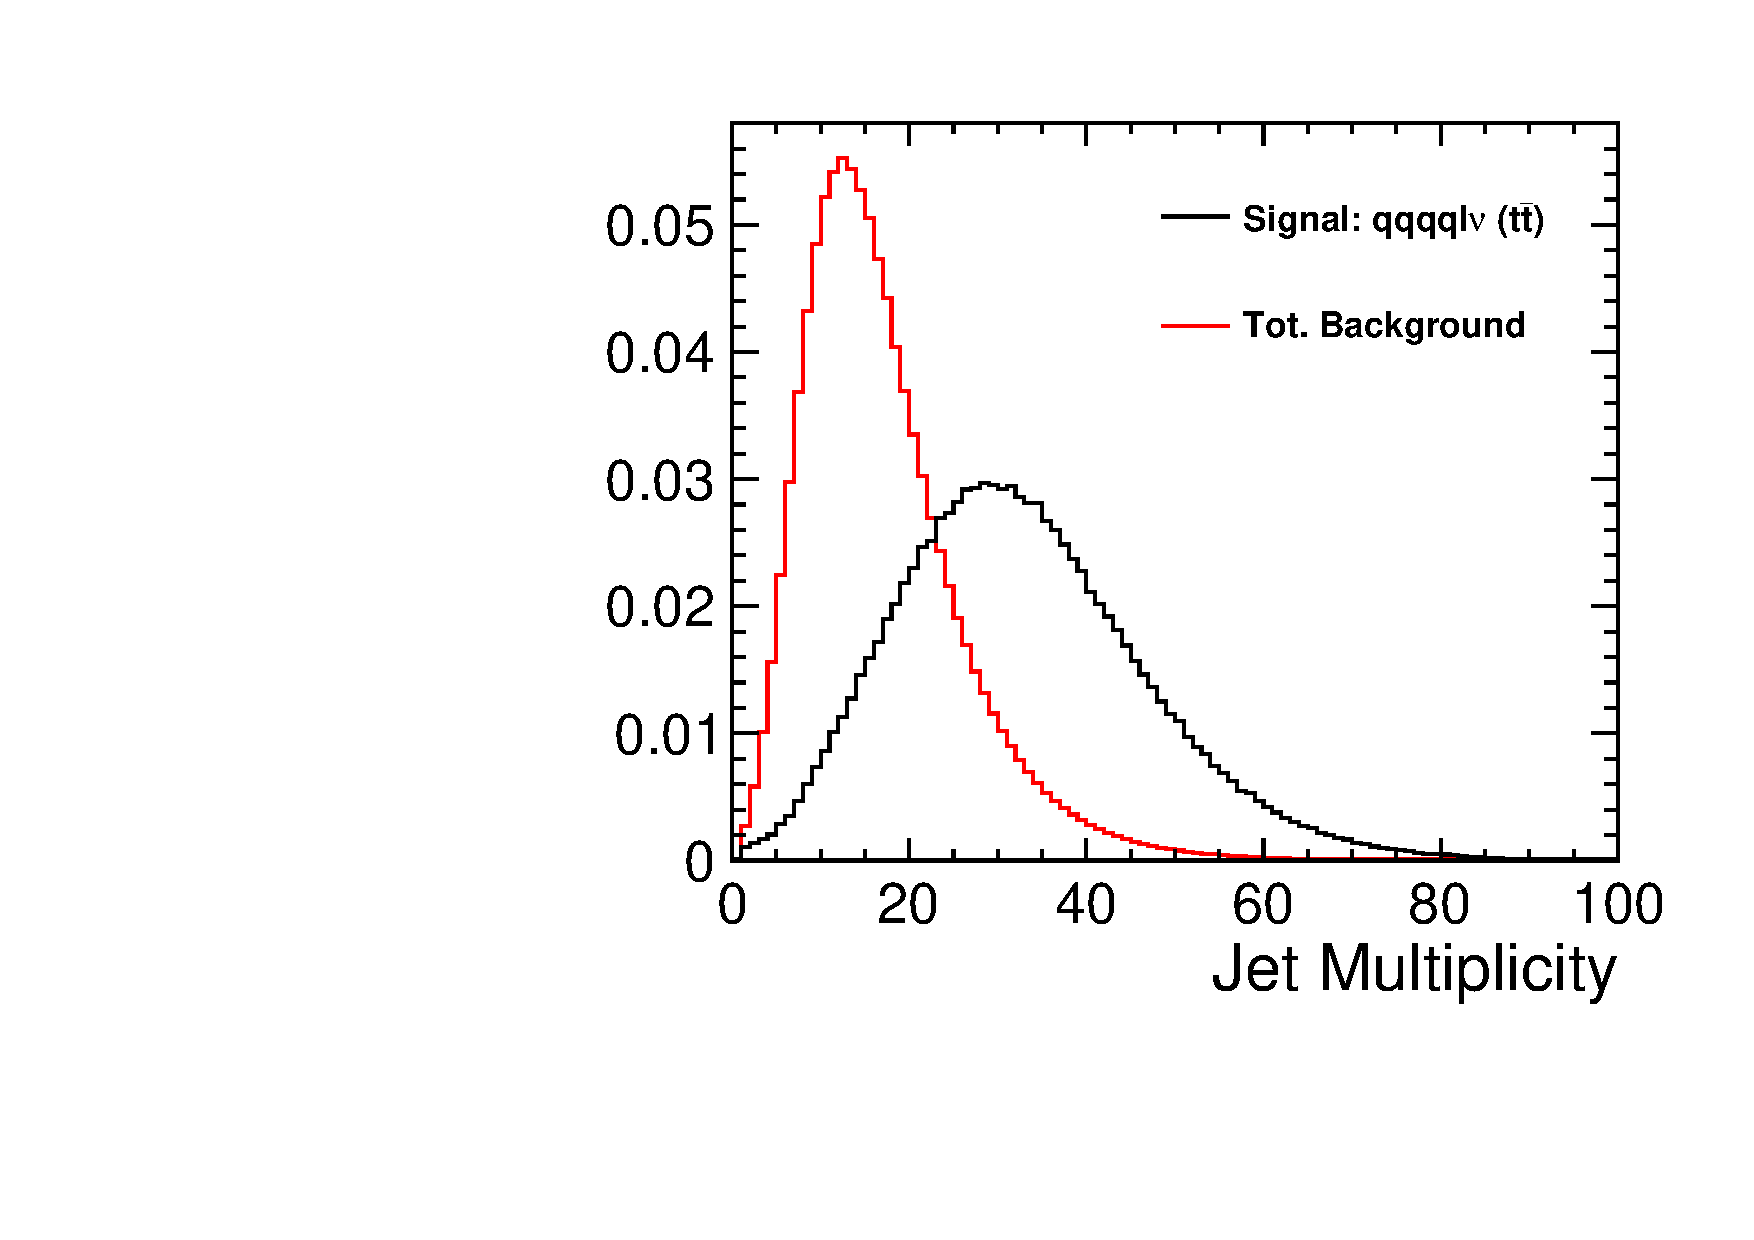
\includegraphics[width=0.8\textwidth]{TopAnalysis/figures/JetMultiplicity.pdf}
  \caption[Jet multiplicity of the hadronic fat jet]{Jet multiplicity of the hadronic fat jet}
  \label{fig:multiplicity}
\end{figure}


The final jet substructure variable that is considered is the jet multiplicity which corresponds to the number of particles within the fat jet. The number of particles produced within a fat jet is proportional to the number of subjets within it. Originally the multiplicity was simply defined as being the number of \ac{PFO}s assigned to the jet during the clustering process. However, to avoid sensitivity to how well the jet hadronization is modeled by PYTHIA, this was replaced by counting the number of ``microjets'' within a fat jet instead, where the microjets are defined by reclustering the fat jet using the kt algorithm in inclusive mode with a small radius R=0.05. This step is effectively reducing the resolution on the number of particles within the fat jet. Ideally one would try using multiple event generators to evaluate the sensitivity of the number of PFOs to the modeling, however as only one event generator is currently available within the linear collider framework this is not an option. To maintain a reduced sensitivity to the jet modeling these microjets are also used in place of PFOs for the N-subjettiness calculations when summing over all particles within a jet. The resulting jet multiplicity for the hadronic fat jet for signal and background events is shown in \reffig{fig:multiplicity}

\subsection{s' Reconstruction}
\label{sec:sprime}
\begin{figure}
  \centering
  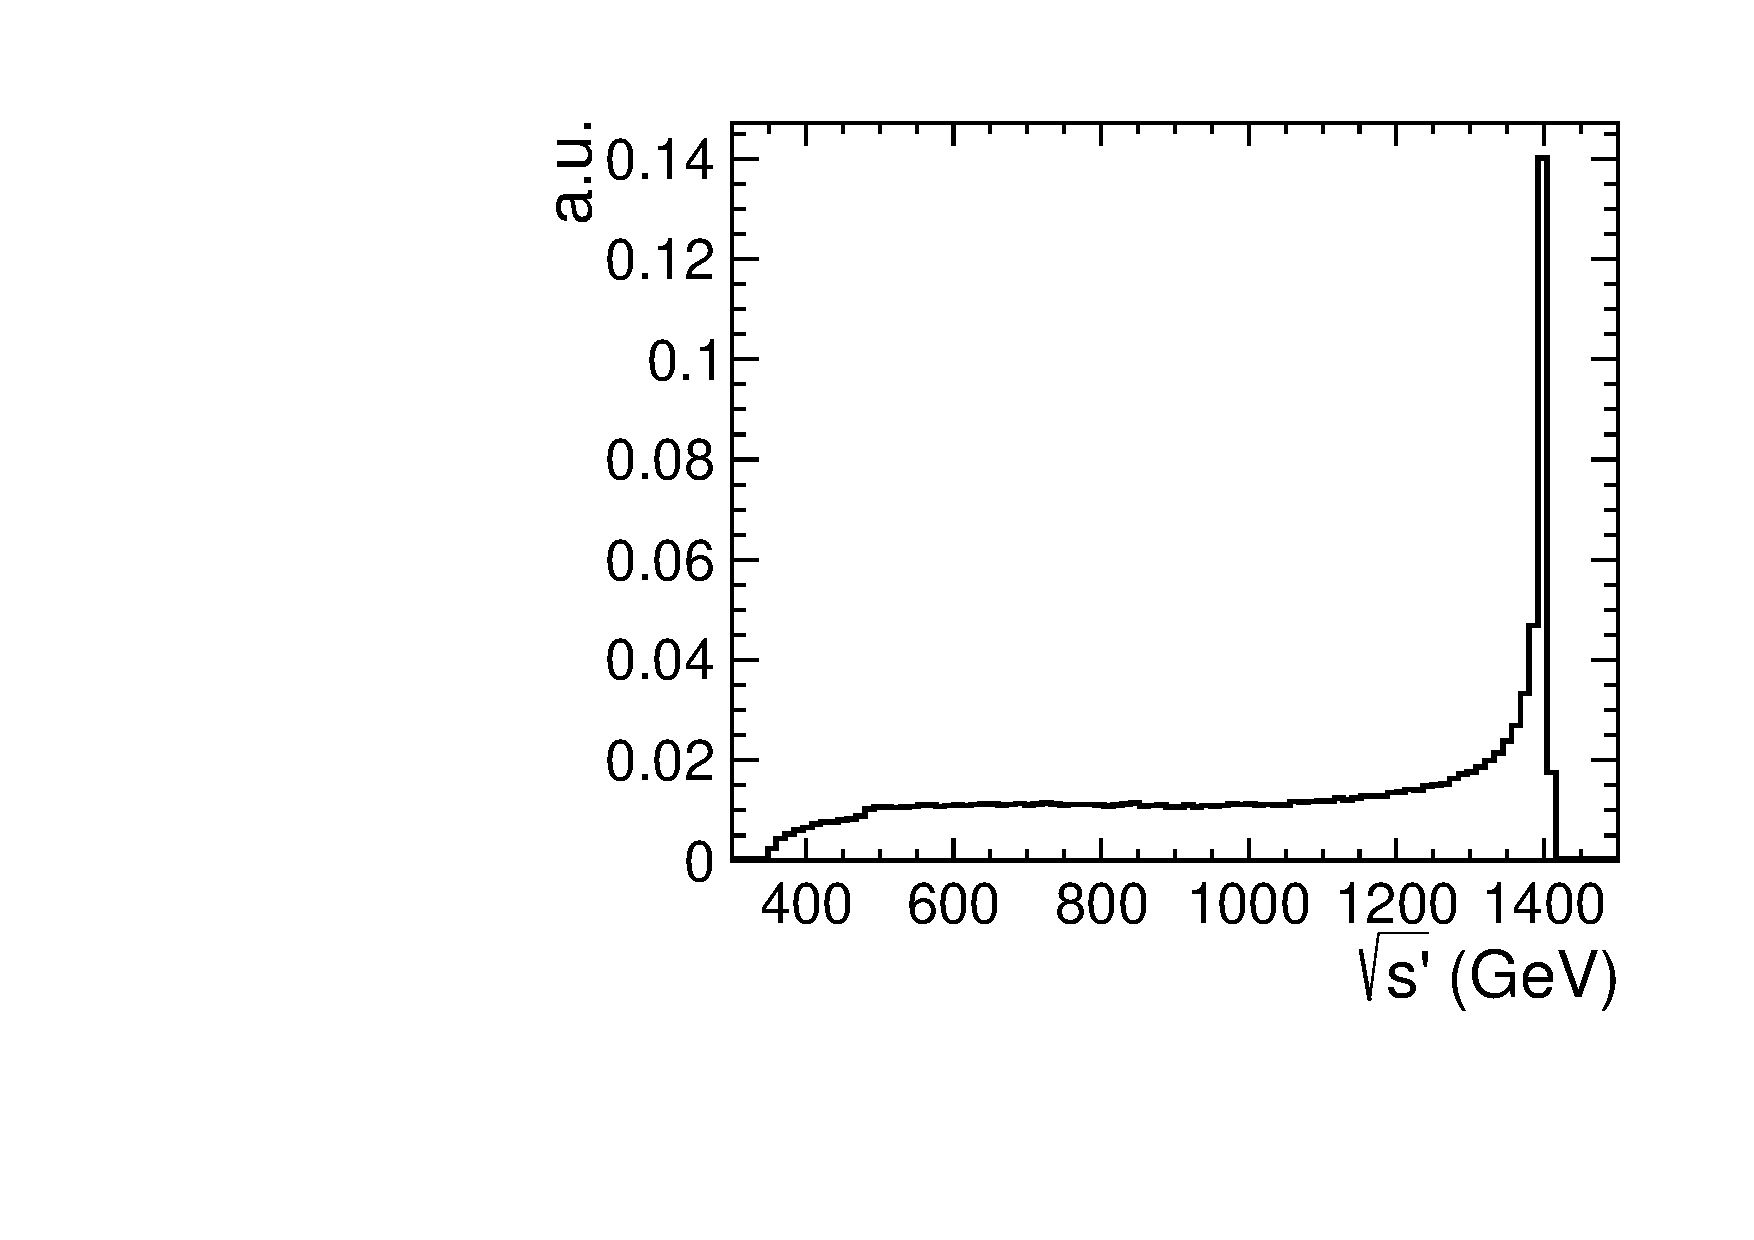
\includegraphics[width=0.6\textwidth]{TopAnalysis/figures/GeneratorSPrime.pdf}
  \caption[Expected $\sqrt{s'}$ spectrum for $t\bar{t}$ at 1.4~TeV]{Expected $\sqrt{s'}$ spectrum for $t\bar{t}$ at 1.4~TeV}
  \label{fig:trueSPrime}
\end{figure}

Following the reconstruction of the lepton and hadronically decaying top it is already possible to calculate $A_{FB}^{t}$, however there are still benefits to first reconstructing the effective centre-of-mass energy of the events (along with the neutrino and any photons produced too).Foremostly this allows a differential measurement of $A_{FB}^{t}$ to be performed. The expected $\sqrt{s'}$ spectrum for $t\bar{t}$ production at 1.4~TeV is shown in \reffig{fig:trueSPrime}. Here it is seen that there is a long tail to the energy spectrum which can be taken advantage of to measure $A_{FB}^{t}$ over a large range of energies. This differential measurement provides greater power for discriminating between physics models than a single $A_{FB}^{t}$ measurement. If $\sqrt{s'}$ can not be reconstructed per event, $A_{FB}^{t}$ would have to either be measured as an integral over the full $\sqrt{s'}$ range or be measured just around the peak energy where there are only small $\sqrt{s'}$ corrections (E $>$ 1200~GeV). However, this would mean discarding $\sim$ 60\% of events produced during the 1.4~TeV run. As well as directly affecting the ways in which we can measure $A_{FB}^{t}$, reconstructing $\sqrt{s'}$ typically involves reconstructing the neutrino and photon contributions in the event. Having a description of these objects can provide further information by allowing the reconstruction of the leptonic top and so could help distinguish signal events from similar backgrounds.

In order to reconstruct $\sqrt{s'}$, multiple methods were attempted with varying complexity. In all cases, combined contributions from \ac{ISR} and \ac{BS} are approximated to the production of one photon radiated from the incoming electron positron pair.

\subsubsection{Transverse/Longitudinal Association}

\begin{figure}
  \centering
  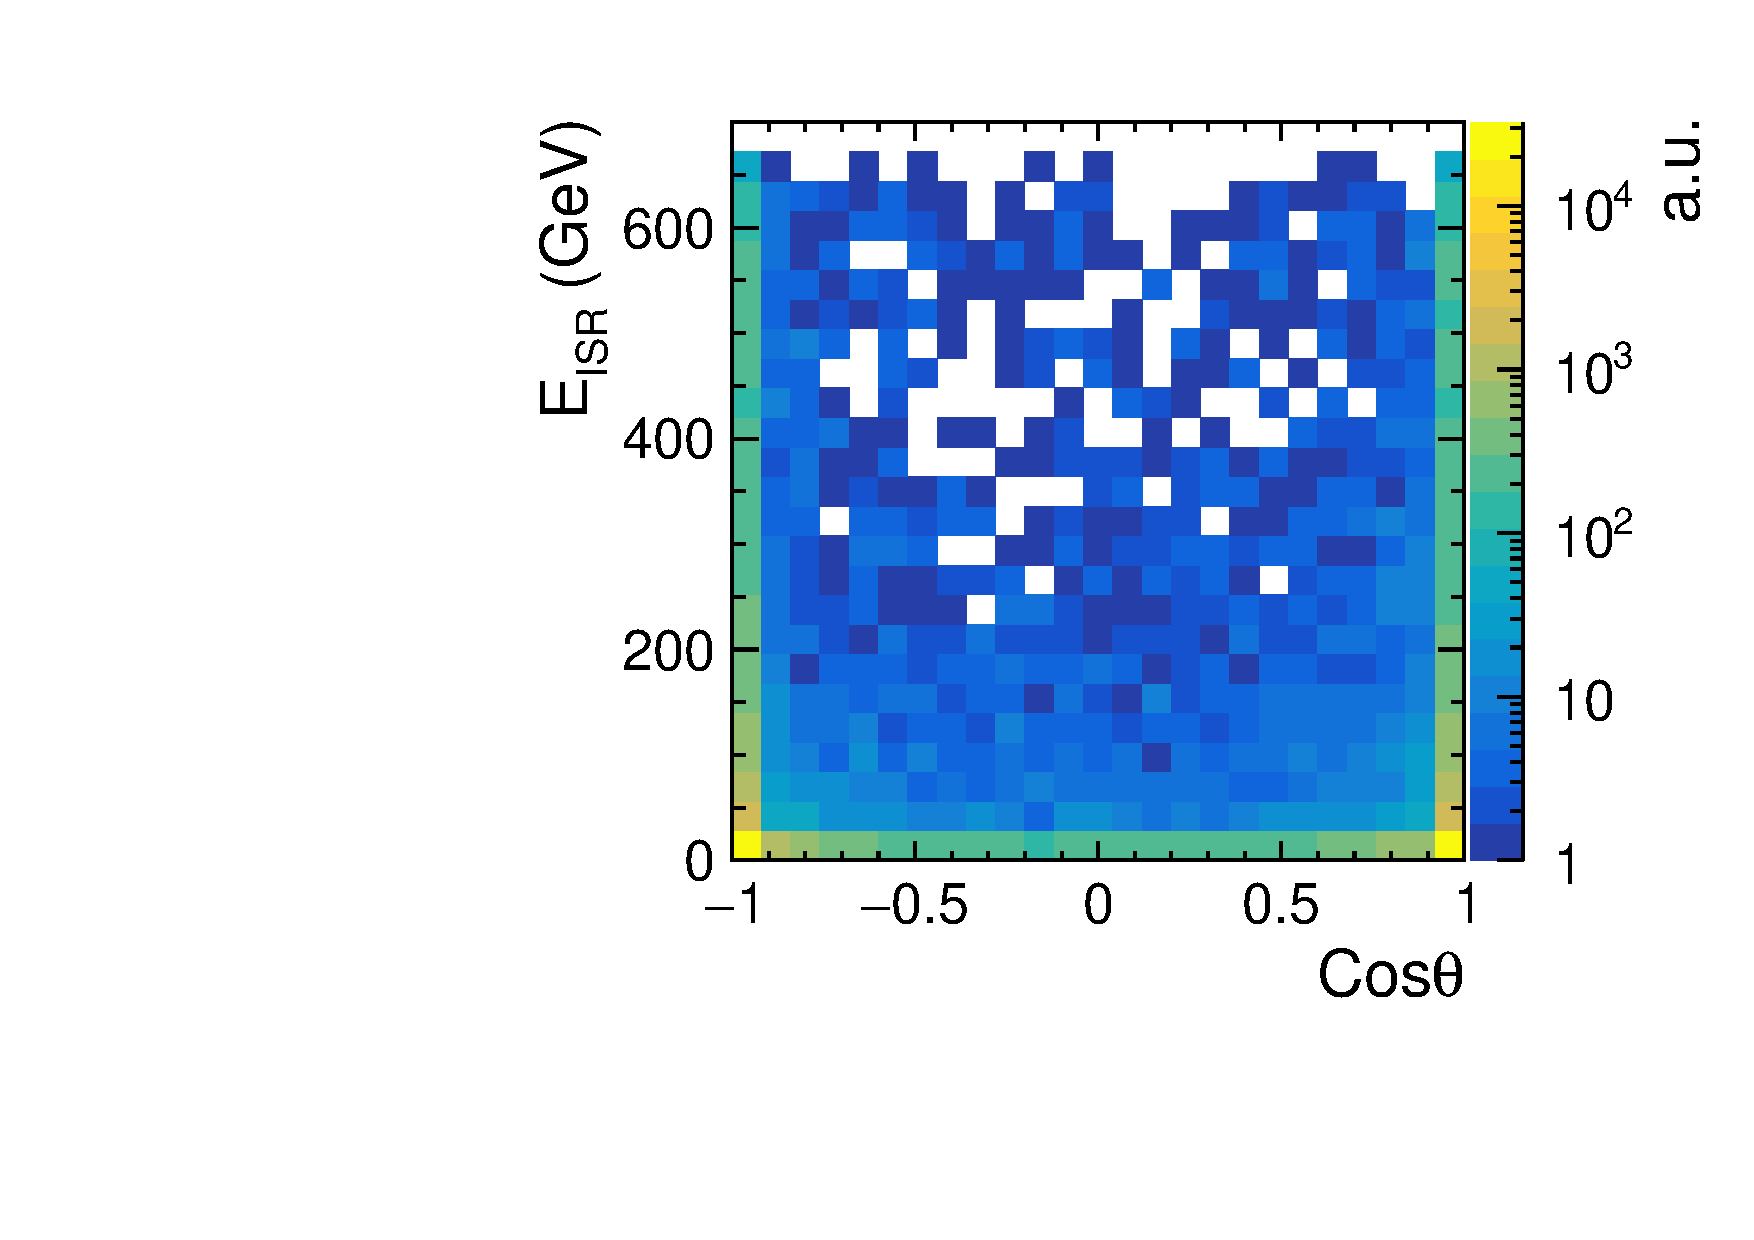
\includegraphics[width=0.6\textwidth]{TopAnalysis/figures/ISRSpectrum.pdf}
  \caption[Angular energy distribution of initial state photons]{Angular energy distribution of initial state photons.}
  \label{fig:photonspectrum}
\end{figure}


The simplest method attempted was to assume that all missing momentum in the transverse direction is attributed to the neutrino, while all longitudinal missing momentum comes from photon contributions. These assumptions are motivated by the results from \reffig{fig:photonspectrum} which show that \ac{ISR} photons are predominantly produced collinear to the beam. Using this method $\sqrt{s'}$ is then taken to be the mass of the neutrino + fat jets system. An event by event comparison of the reconstructed $\sqrt{s'}$ to the generator $\sqrt{s'}$ is shown in \reffig{fig:simpleAssoication}. Overall this method is unsatisfactory as the reconstructed $\sqrt{s'}$ is consistently underestimating the true $\sqrt{s'}$ of the event. This should be expected as the assumption that the photon losses are collinear to the beam is only approximately true. We have shown that it is true for high energy \ac{ISR} photons, however one can see from \reffig{fig:photonspectrum} that for lower energy emissions the photons can be emitted at large angles relative to the beam. This is why there is a stronger correlation between the reconstructed and generator $\sqrt{s'}$ when the photon energy losses are largest. On top of this there will also be photons produced through \ac{BS} and there is no reason to assume these would be produced with negligible transverse momentum. In practice the neutrino from the leptonic top decay will also have a non negligible longitudinal momentum that should be accounted for. Overall it is clear that this method is unsatisfactory for reconstructing $\sqrt{s'}$.

\begin{figure}
  \centering
  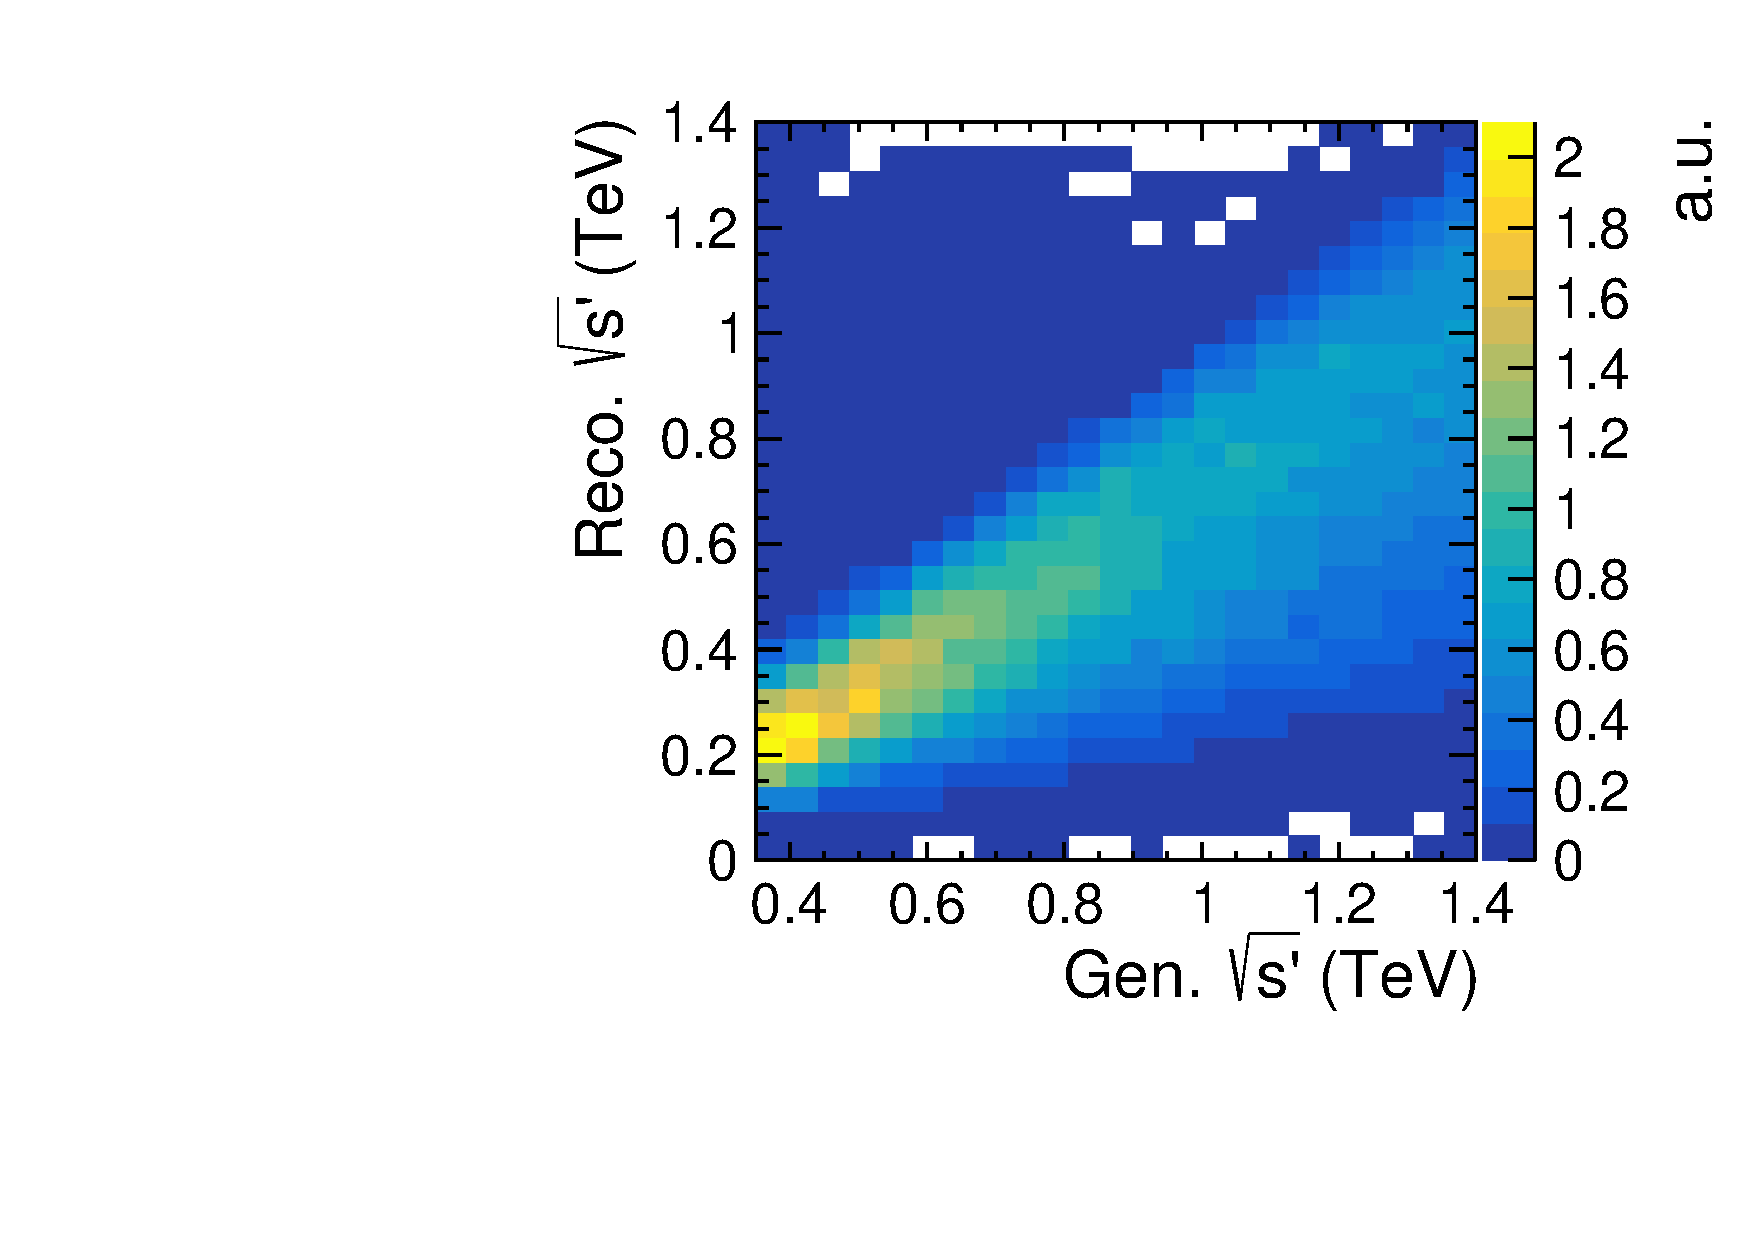
\includegraphics[width=0.6\textwidth]{TopAnalysis/figures/CrudeEVsTrueE.pdf}
  \caption[Reconstructed $\sqrt{s'}$ vs generator $\sqrt{s'}$ for transverse/longitudinal association method]{Reconstructed $\sqrt{s'}$ vs generator $\sqrt{s'}$ for transverse/longitudinal association method.}
  \label{fig:simpleAssoication}
\end{figure}

\subsubsection{Analytic Mass Constraint}

\begin{figure}
  \centering
  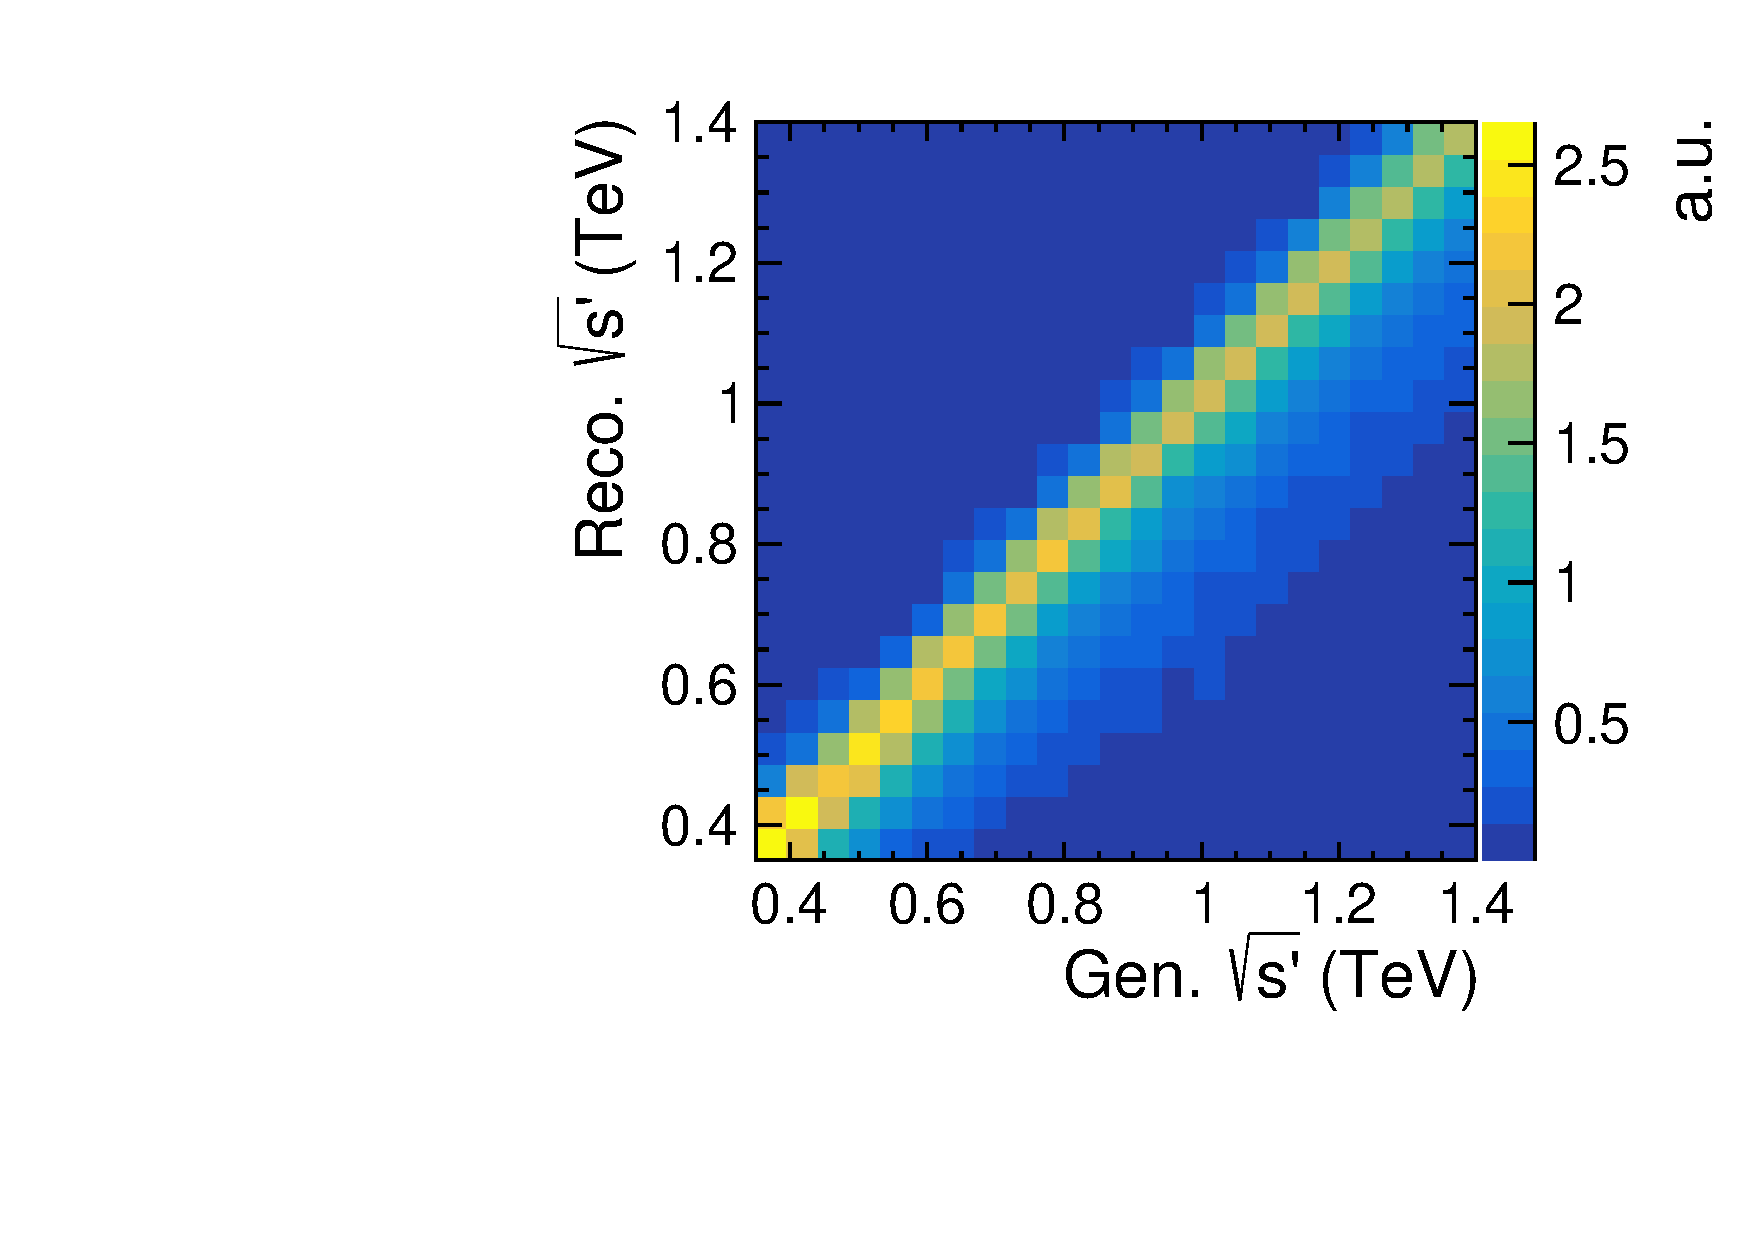
\includegraphics[width=0.6\textwidth]{TopAnalysis/figures/AnalEVsTrueE.pdf}
  \caption[Reconstructed $\sqrt{s'}$ vs generator $\sqrt{s'}$ for mass constraint method]{Reconstructed $\sqrt{s'}$ vs generator $\sqrt{s'}$ for mass constraint method.}
  \label{fig:MassConstraint}
\end{figure}
\begin{figure}
  \centering
  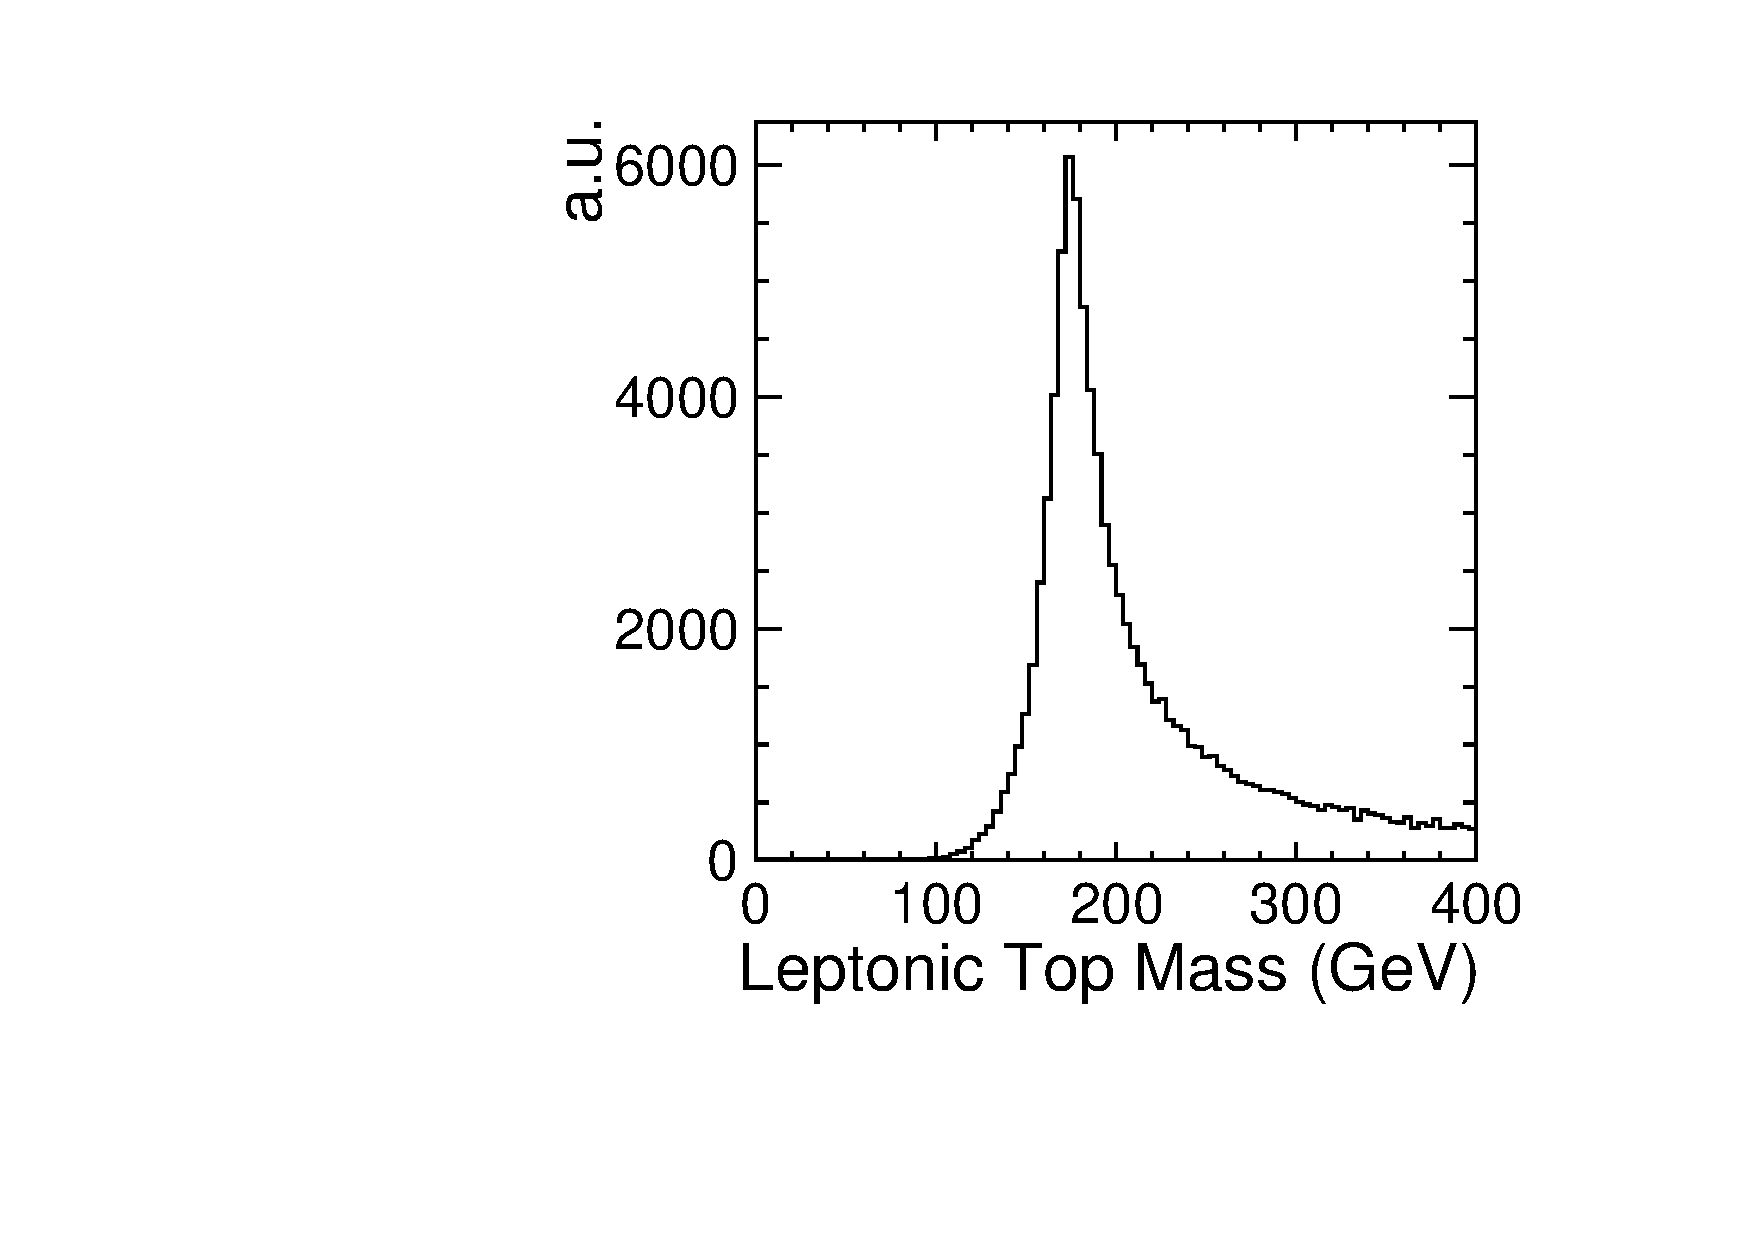
\includegraphics[width=0.6\textwidth]{TopAnalysis/figures/AnalTopMass.pdf}
  \caption[Mass of reconstructed leptonic top when using mass constraint method]{Mass of reconstructed top when using mass constraint method.}
  \label{fig:TopMassFrommassMethod}
\end{figure}

The second method attempted is an adaptation of the first method that makes use of the high efficiency with which the lepton is reconstructed to improve the performance. This method was introduced in \ac{CLIC} studies by a fellow member of the CLICdp group working on the alternative version of this analysis\cite{TopPaperDraft}. It starts in the same manner by attributing all transverse missing momentum to the neutrino, however the missing longitudinal momentum is then divided between the neutrino and photon. This is done by constraining the $z$ component of the neutrino momentum by insisting the combination of the lepton and neutrino four momenta reproduces the W mass. Overall this acts to remove the incorrect assumption that the neutrinos longitudinal momentum is negligible compared to the photons. The details of the calculations are as follows:

\begin{equation}
  p_W=p_l+p_\nu
\end{equation}
\begin{equation}
M_W^2=M_l^2 + 2(E_lE_\nu - \mathbf{p_l.p_\nu})
\end{equation}
\begin{equation}
0=-\frac{M_W^2-M_l^2}{2} + E_l.\sqrt{p^2_{\nu , x}+p^2_{\nu , y}+p^2_{\nu , z}} - (p_{\nu , x}p_{l , x}+p_{\nu , y}p_{l , y}+p_{\nu , z}p_{l , z})
\end{equation}
\begin{equation}
p_{\nu , z}=\frac{1}{2(p^2_{l , x}-E^2_{l})} (p_{l , z}(M_l^2-M_W^2)-2p_{l , z}(p_{l , x}p_{\nu , x}+p_{l , y}p_{\nu , y}) + X)
\end{equation}
Where,
\begin{equation}
  \label{eq:X}
  X=\sqrt{E_l^2((M_W^2-M_l^2 +2(p_{l , x}p_{\nu , x}+p_{l , y}p_{\nu , y}))^2 +4\epsilon_T^2(p^2_{l , z}-E_l^2) )}
\end{equation}
\begin{equation}
  \epsilon_T=\sqrt{p^2_{\nu , x}+p^2_{\nu , y}}
\end{equation}

In the event that X is imaginary, $\epsilon_T$ is scaled so that X=0. The key detail however, is that there are two possible solutions for the neutrino momentum arising from the quadratic form of \refeq{eq:X}. To decide the most suitable solution the W is combined with a fat jet (adding two more possible solutions, one for each fat jet) and the solution found to give an invariant mass closest to the top mass is chosen to be best. The resulting reconstructed leptonic top mass and $\sqrt{s'}$ reconstruction performance are shown in \reffigs{fig:MassConstraint} and \ref{fig:TopMassFrommassMethod}. The method does still have certain flaws that result in misreconstruction such as the assumption that all missing transverse momentum comes from the neutrinos and that the W mass is exactly 80.4 GeV with no associated width, however it clearly offers an improvement over the first method with a reasonable degree of agreement seen across the full $\sqrt{s'}$ range and a lower tendency to underestimate $\sqrt{s'}$.

\subsubsection{Collinearity}

An alternative solution that was proposed was to use the collinearity (angular separation) of the $t\bar{t}$ pair as a way to measure $\sqrt{s'}$. For collisions occurring at the nominal collision energy, the total momentum of the collision should be zero and so the two tops are produced back to back in the lab frame. If a photon is emitted before the electron positron collision occurs, the $t\bar{t}$ pair will have a none zero momentum and so will be boosted resulting in a reduced angular separation between the two tops. The scale of the boost (and thus the size of the angular separation) is proportional to the total momentum of the photon and so should be proportional to $\sqrt{s'}$. Extraction of $\sqrt{s'}$ is performed by first using one sample to determine the exact relationship between the collinearity and the generator $\sqrt{s'}$. This relationship is shown in \reffig{fig:Collinearity}. A calibration curve is then generated by fitting the profile of this with a second order polynomial. The performance is evaluated by taking a second event sample and using the calibration curve to map back from the collinearity to a reconstructed $\sqrt{s'}$. The resulting distribution for reconstructed $\sqrt{s'}$ vs generator $\sqrt{s'}$ is shown in \reffig{fig:CollinearitySPrime}. Clearly this method is not as performant as the analytical method. One of the main reasons for this is that the collinearity should be measured between the two tops, however due to the neutrino not being reconstructed in the leptonic decay, one of the objects used for measuring the collinearity will be incomplete. This reduces the correlation between the collinearity and $\sqrt{s'}$. Further, as $\sqrt{s'}$ decreases and the tops become less well separated, the chance of reconstruction failures occurring increases. In addition, the jet finding approach used will start to mix parts of each top when trying to construct two fat jets and so the objects the collinearity is calculated for will no longer correspond to the generator level tops (see \refsec{sec:jetassociation}.) This explains the very poor performance for the lowest $\sqrt{s'}$ events.

\begin{figure}
  \centering
  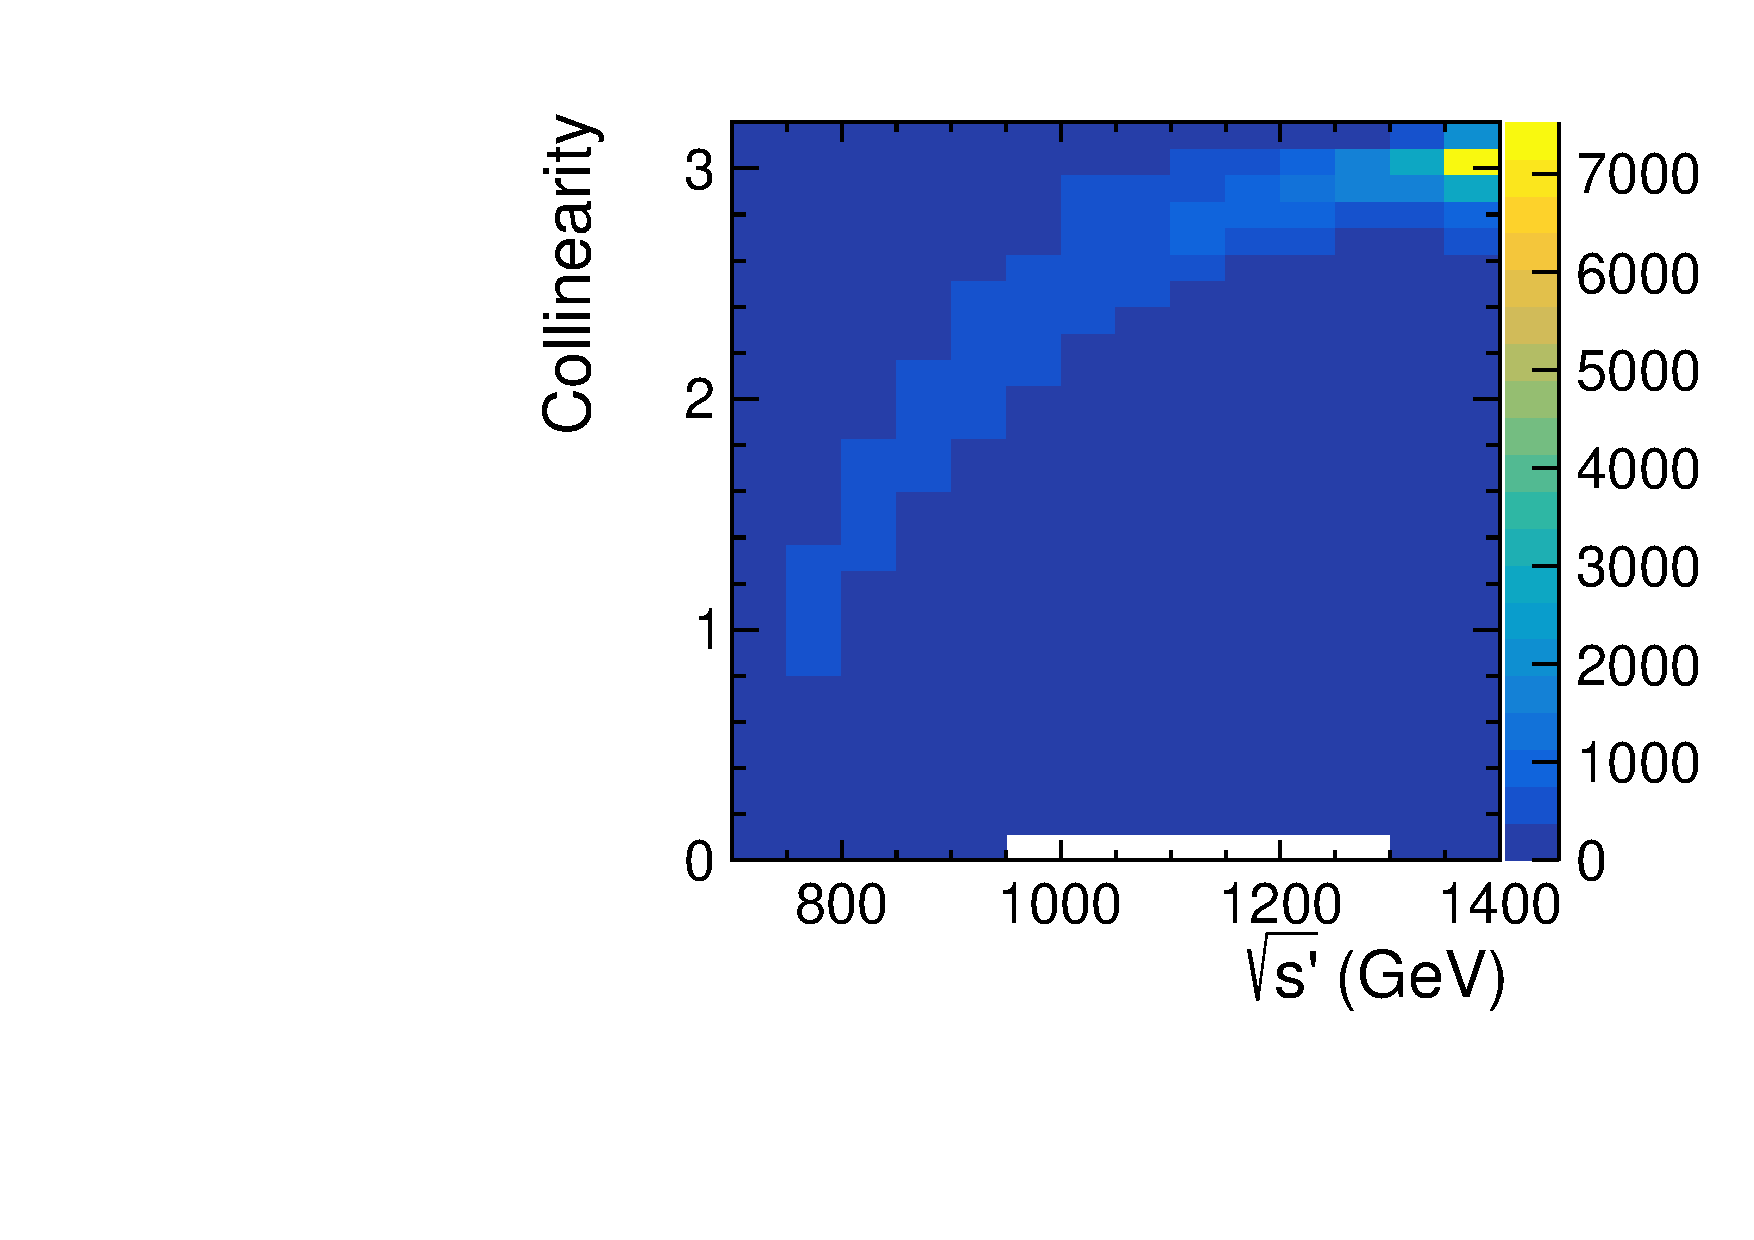
\includegraphics[width=0.6\textwidth]{TopAnalysis/figures/ColVsE.pdf}
  \caption[Collinearity of $t\bar{t}$ pair]{Collinearity of the $t\bar{t}$ pair.}
  \label{fig:Collinearity}
\end{figure}

\begin{figure}
  \centering
  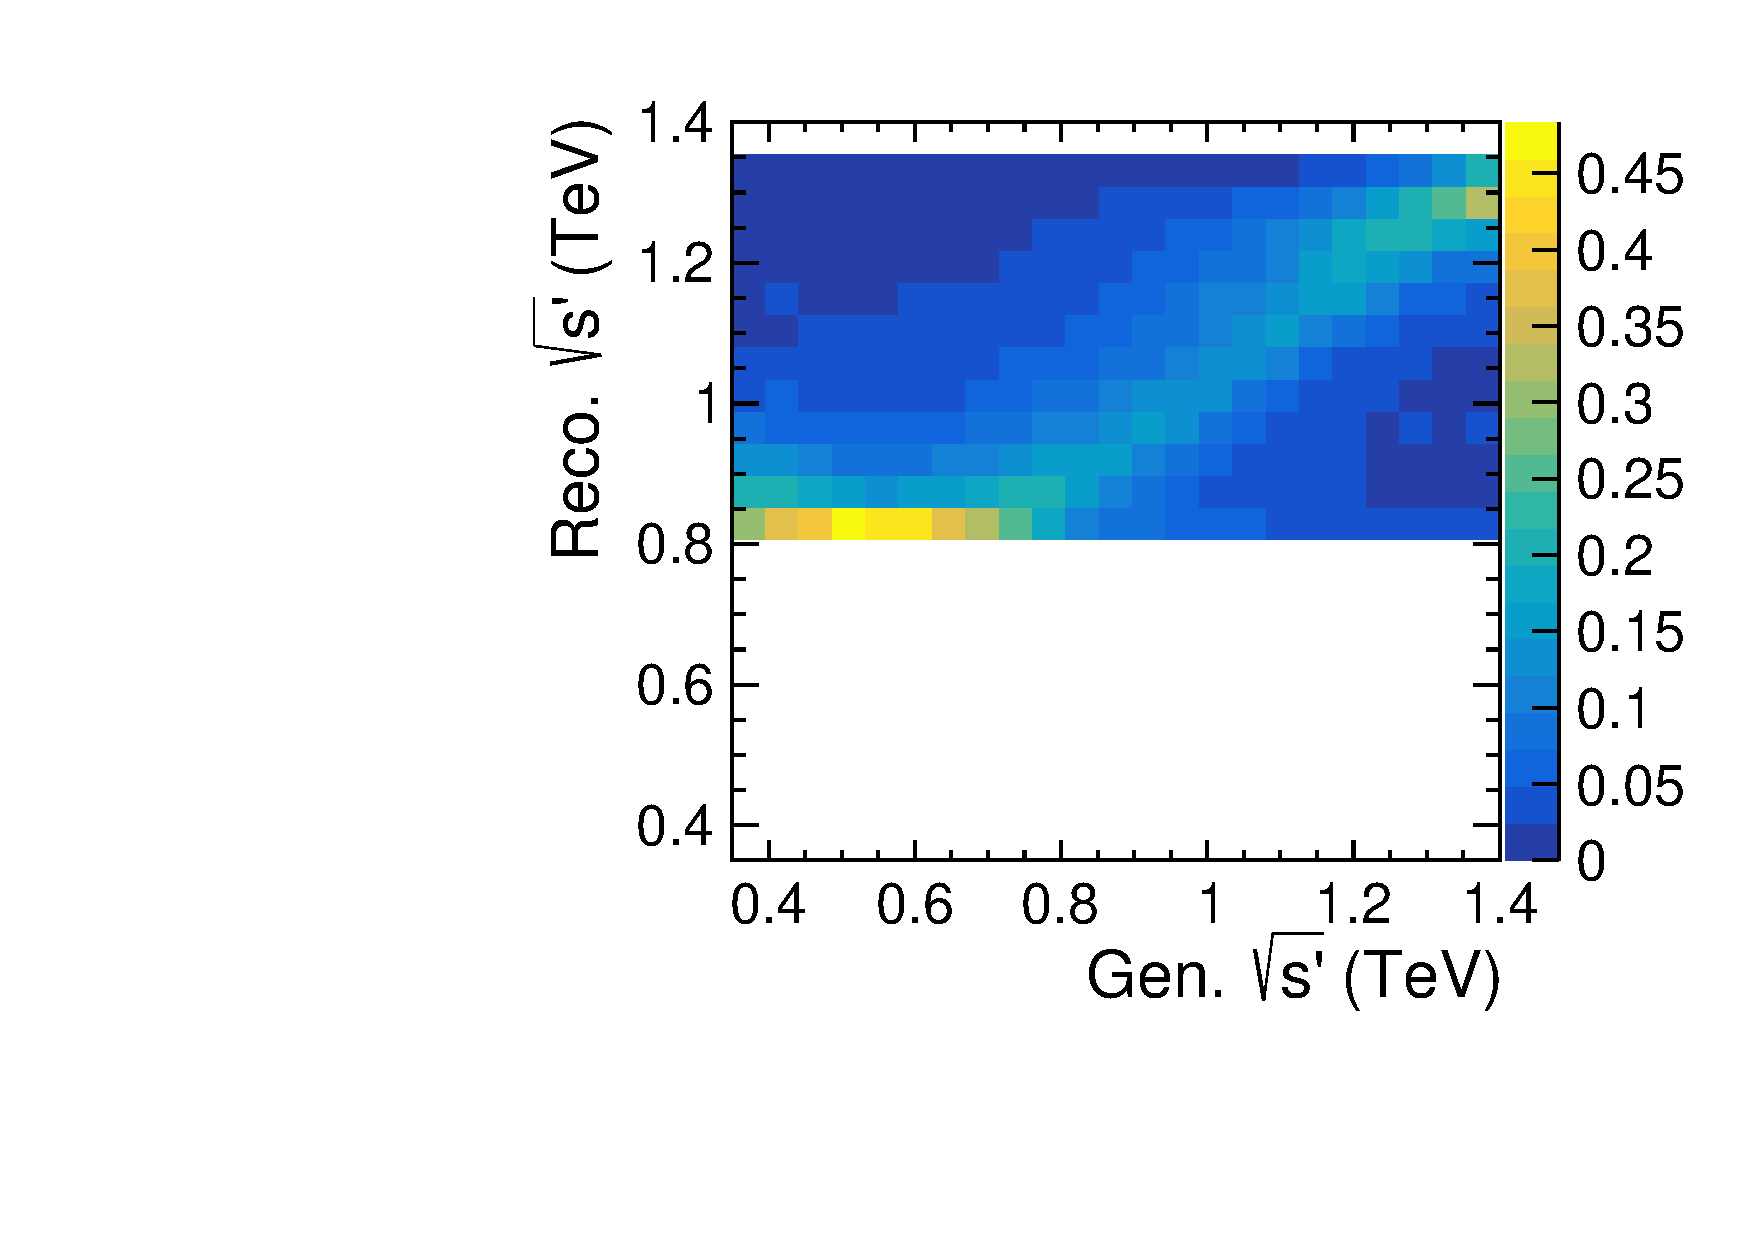
\includegraphics[width=0.6\textwidth]{TopAnalysis/figures/ColEVsTrueE.pdf}
  \caption[Reconstructed $\sqrt{s'}$ vs generator $\sqrt{s'}$ for collinearity method]{Reconstructed $\sqrt{s'}$ vs generator $\sqrt{s'}$ for collinearity method.}
  \label{fig:CollinearitySPrime}
\end{figure}

\subsubsection{Kinematic Fitting}

The final approach considered was to use a constrained kinematic fitter (MarlinKinFit v00-03\cite{List:88030}) to simultaneously determine the photon and and neutrino four momenta. The fit has four free parameters: the neutrino's three-momentum and the photons $z$ momentum (it is still assumed that photons have negligible transverse momentum), and has six constraints: the total four momentum of the system, the mass of the leptonically decaying W and that the masses of the two tops are consistent. It would be possible to replace the last constraint with a target mass for each top, however the current form has the benefit that it requires no prior knowledge of the mass of the top. The fit is passed five fit objects: the isolated lepton, two fat jets, neutrino and photon.  It will then try and find a solution that satisfies all the fit constraints by varying the four momenta of the fit objects. In the case of the physically observable objects (the lepton and jets), the variation of the four momenta is limited according to the relevant detector resolutions:

\begin{align}
  \sigma_{E, Had}&=35\%\sqrt{E}
  \\
  \sigma_{E, EM}&=20\%\sqrt{E}
\\
  \sigma_{\theta/\phi}&=10\%
\end{align}

The photon power spectrum is also introduced within the fit by setting the parameter $b$ in the following formula:

\begin{equation}
\frac{dN}{dp_z}\propto\frac{1}{p_z^{1-b}}
\end{equation}

A value of $b$=0.5 was found to give the best agreement for the reconstructed and generator $\sqrt{s'}$. The resulting performance is shown in \reffig{fig:KinFit}. Overall the performance is similar to that of the analytic method with a good agreement seen between the reconstructed and generator $\sqrt{s'}$ across the full $\sqrt{s'}$ spectrum. It was decided that this method shall be used for $\sqrt{s'}$ determination for the rest of the analysis. While the analytical method is as performant, it is potentially less robust than the kinematic fitting due to the fact it uses a fixed top mass and is unable to scale the four momenta of the measured particles to compensate for detector resolutions.  For the rest of the analysis, the four momenta of all objects are taken to be those returned by the kinematic fit.

\begin{figure}
  \centering
  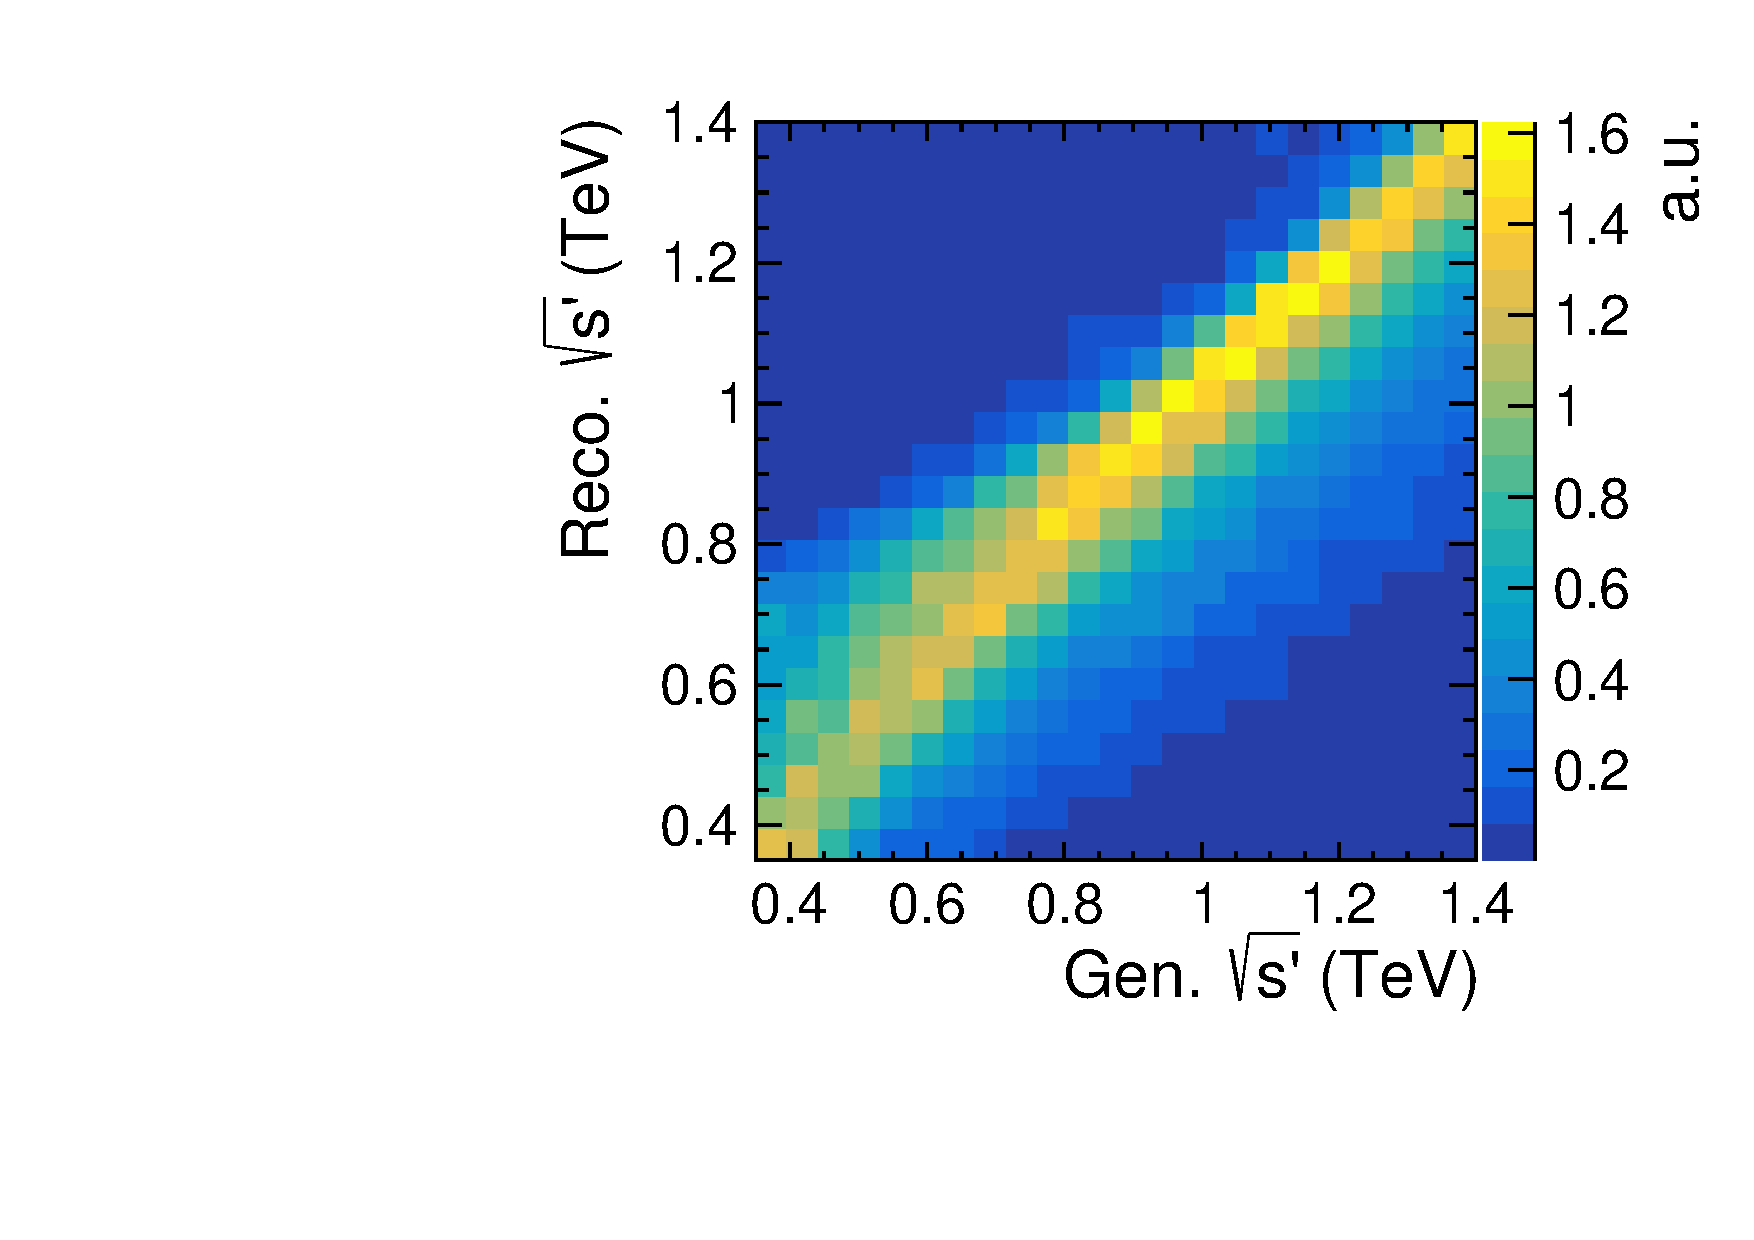
\includegraphics[width=0.6\textwidth]{TopAnalysis/figures/KinEVsTrueE.pdf}
  \caption[Reconstructed $\sqrt{s'}$ vs generator $\sqrt{s'}$ for kinematic fit  method]{Reconstructed $\sqrt{s'}$ vs generator $\sqrt{s'}$ for kinematic fit method.}
  \label{fig:KinFit}
\end{figure}

\subsection{Flavour Tagging}
\label{Flavour Tagging}

\begin{figure}[t]
  \centering
  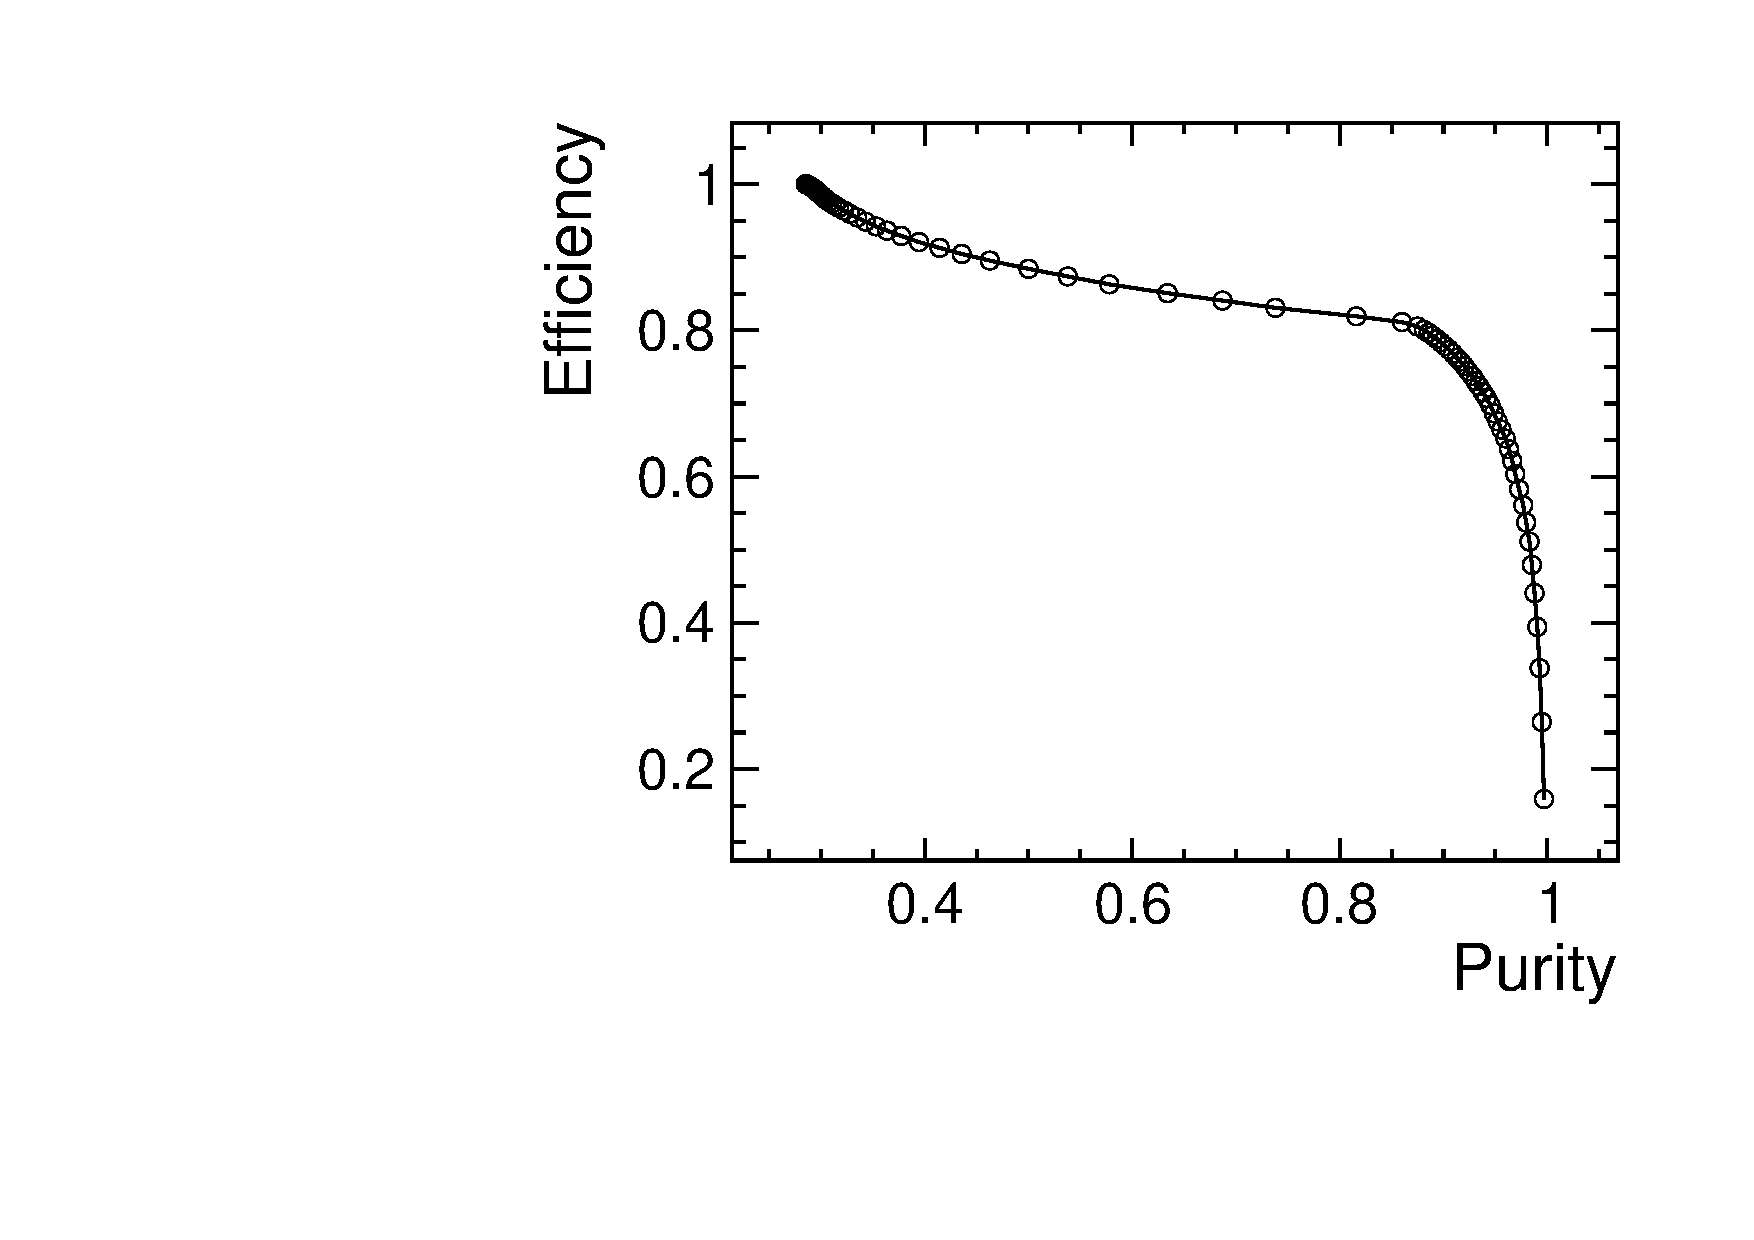
\includegraphics[width=0.78\textwidth,height=7cm,keepaspectratio]{HiggsAnalysis/figures/updatedpurityvsefficiency.pdf}
  \caption[B-Tagging Purity vs Efficiency]{Purity vs efficiency for identifying b-jets, obtained from a sample of Z$\rightarrow$ light, c and b quark events simulated at $\sqrt{s}=$1.4 TeV.}
  \label{fig:Zbtagging}
\end{figure}

Flavour tagging was performed using LCFIPlus v00-05-02\cite{Suehara:2015ura}. LCFIPlus makes use of three BDTs dedicated to searching for u/d/s (light), b and c quarks respectively, to provide a b-tag and c-tag indicating the probability of a jet containing a b or c quark. As the signal process contains two b jets, only the results of the b-tag are considered here. The BDTs were trained using 50,000 $ee\rightarrow Z\nu\nu, Z\rightarrow qq$ events generated at 1.4~TeV each . The base performance of the BDTs was assessed using a further 150,000 $ee\rightarrow Z\nu\nu, Z\rightarrow qq$ events containing an even mixture of bb, cc and light quarks to measure the efficiency and purity that could be obtained. The results of this test (shown in \reffig{fig:Zbtagging}) indicate that in the case of Z$\rightarrow$qq events high efficiencies and purities of $\sim$85\% can be achieved simultaneously. Before applying the flavour tagging to our analysis the events are first reclustered into four jets to try and capture the bjets separately from the light quark jets. This is done within the LCFIPlus package which uses the Durham algorithm by default. Ideally the BDTs would also be retrained using top events rather than Z, however due to limited sample sizes this was not a realistic option. The performance of the btagging for semileptonic top events was evaluated by comparing the highest and second highest b-tags assigned to any of the four jets in signal events to those in backgrounds. The results of this comparison are seen in \reffig{fig:btagging}. It is clear that the btagging is consistently successful in finding the first b jet, but is less reliable for finding a second b jet. This is expected due to the topology of the event. The b jet produced by the leptonically decaying top should be well isolated from other hadronic jets in the final state and the charged lepton is identified and removed with high efficiency whereas the bjet from the hadronically decaying top will be close to two other jets meaning the jet finder is less likely to accurately associate the PFOs in that region with the correct initial quark. As a result the b jet from the leptonic side should be consistently reconstructed and tagged whereas the b jet on the hadronic side will be less consistent as the efficiency for reconstructing the jet correctly is much lower. Despite the poorer performance of the second highest b-tag, both variables provide clear potential as discriminating variables for removing background. 


\begin{figure}
  \centering
  \begin{subfigure}{.5\textwidth}
    \centering
    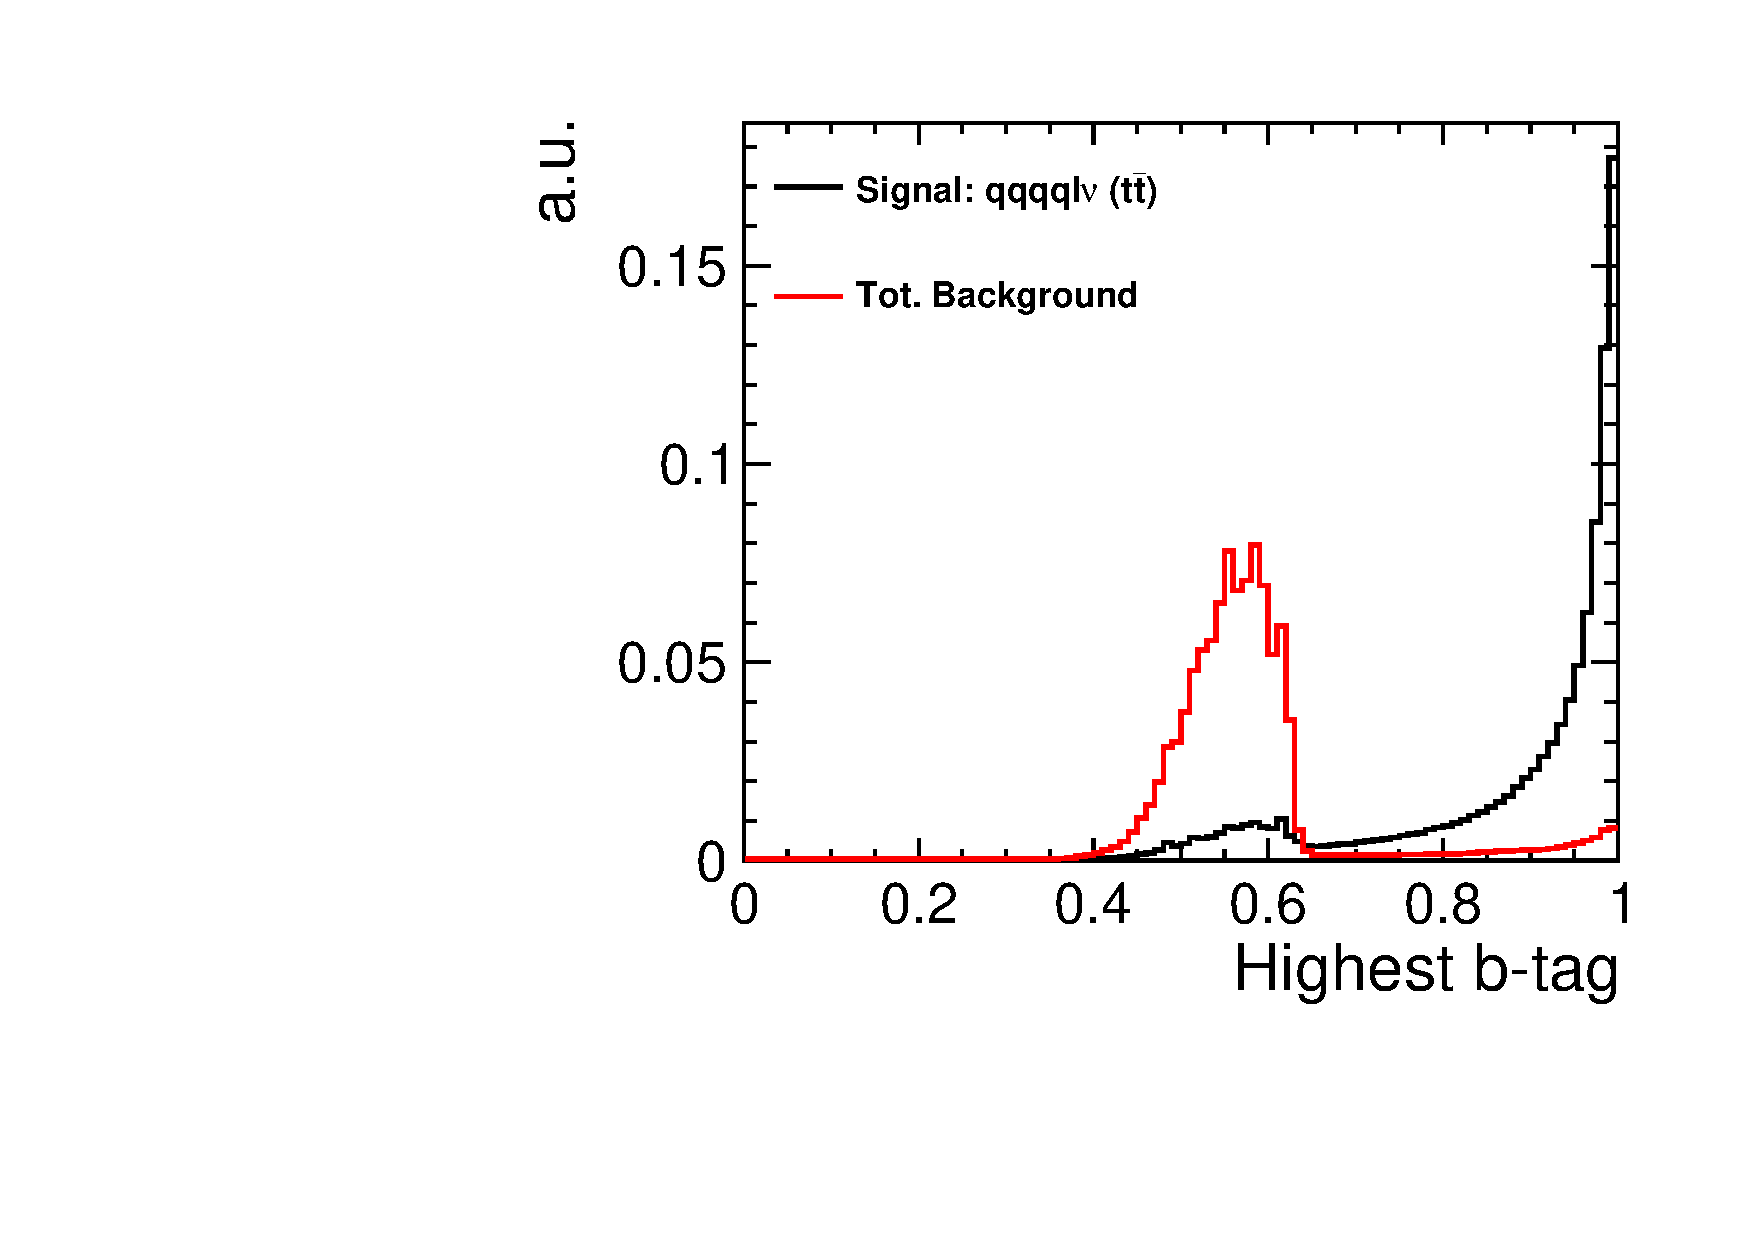
\includegraphics[width=0.99\textwidth]{TopAnalysis/figures/HighestBTag.pdf}
    \caption[Highest b-tag in event]{Highest b-tag in event}
  \end{subfigure}%
  \begin{subfigure}{.5\textwidth}
    \centering
    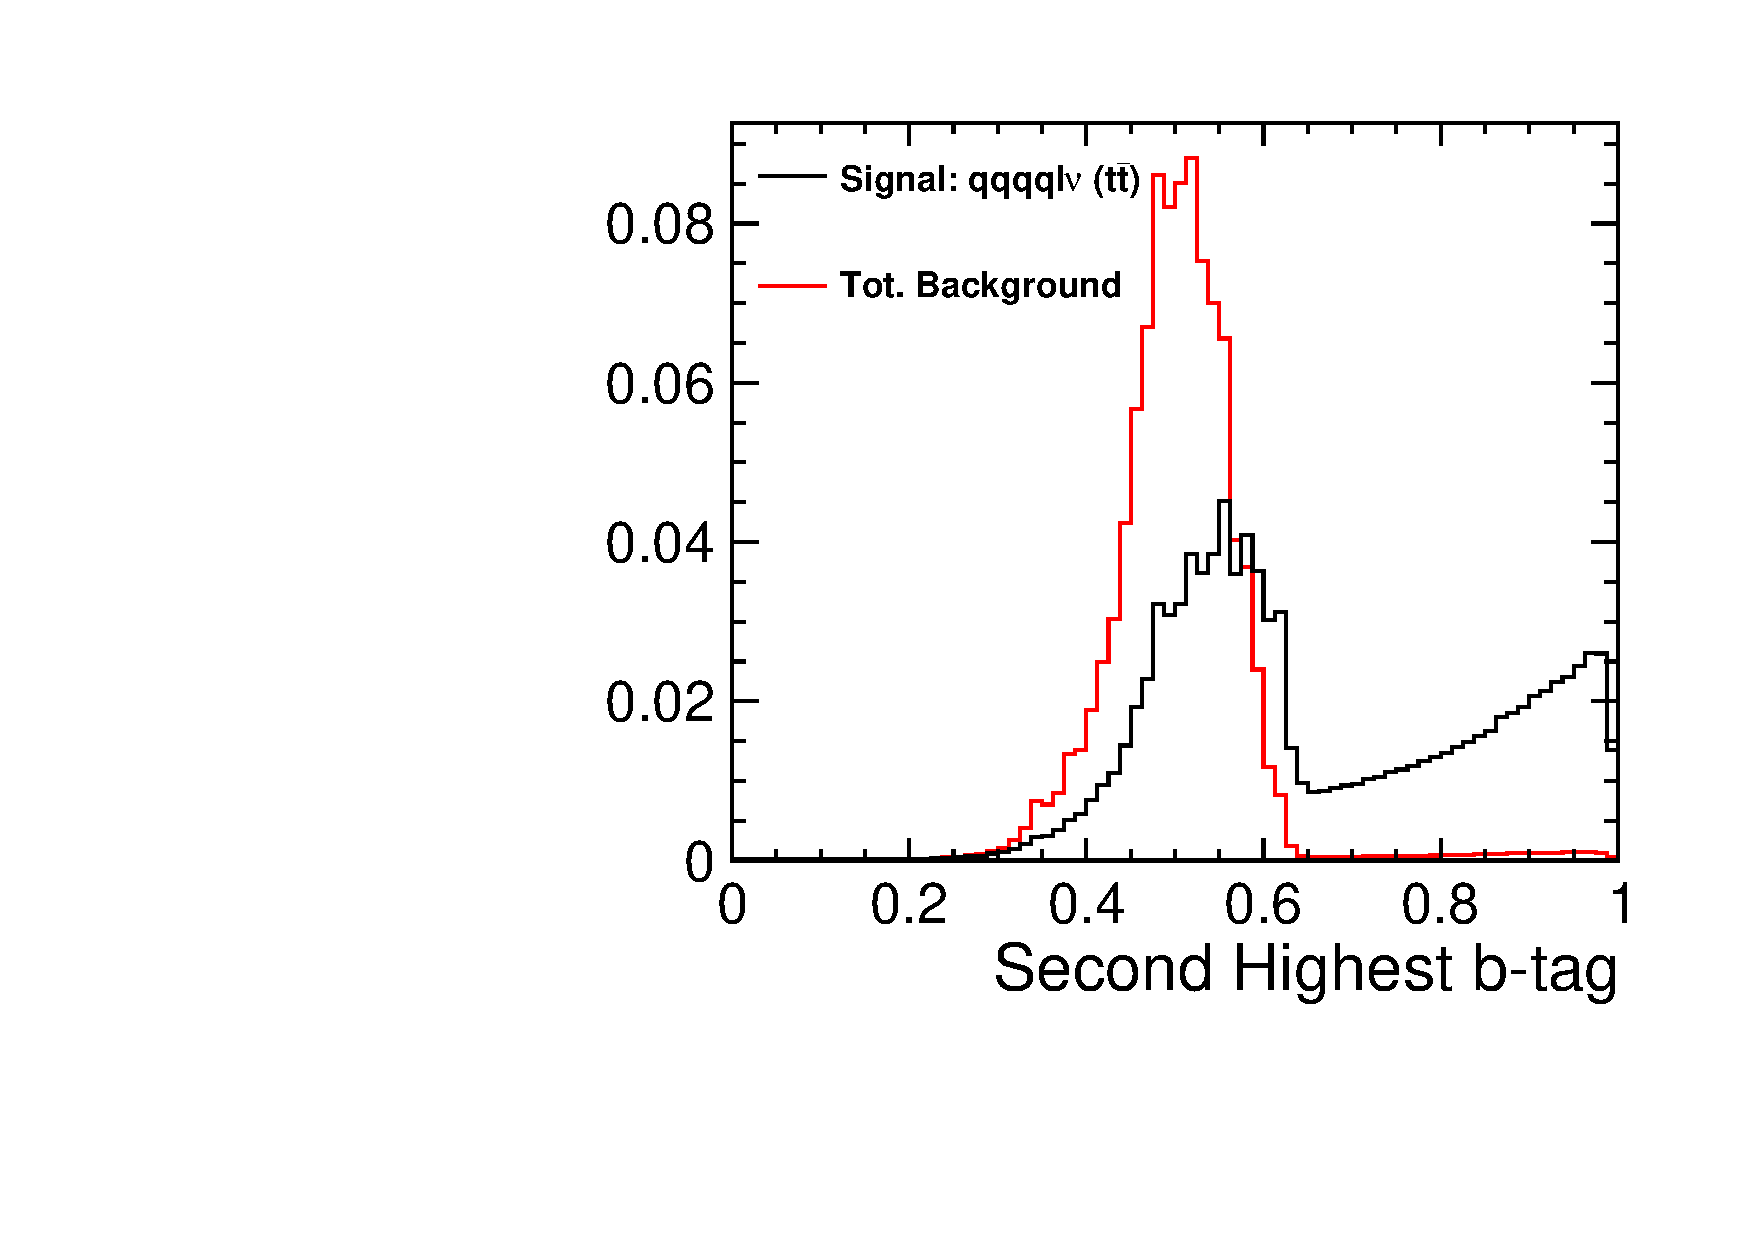
\includegraphics[width=0.99\textwidth]{TopAnalysis/figures/NextHighestBTag.pdf}
    \caption[Second highest b-tag event in event]{Second highest b-tag in event}
  \end{subfigure}
  \caption[B-Tagging performance]{B-Tagging performance.}
  \label{fig:btagging}
\end{figure}


\section{Methods For Calculating $A_{FB}^t$}
\label{Calculating AFB}

In it's simplest form, $A_{FB}^t$ is defined as being:

\begin{equation}
A_{FB}^t=\frac{N_F-N_B}{N_F+N_B}
\end{equation}

However for the purpose of measuring the asymmetry to the greatest precision possible, it can be better defined in terms of the differential top pair production cross section\cite{PhysRevD.25.1218}:

\begin{equation}
  \label{eq:afbfit}
\frac{\mathrm{d}\sigma}{\mathrm{d}\cos\theta} \propto \frac{3}{8}(1+\cos^{2}\theta)\sigma_{U} + \frac{3}{4}(1-\cos^{2}\theta)\sigma_{L} + A_{FB}^{t}\cos\theta\sigma_{Tot}
\end{equation}

where $\sigma_U$, $\sigma_L$ and $\sigma_{Tot}$ correspond to the unpolarised, longitudinally polarised and total cross section respectively and $\theta$ is the production angle of the top relative to the incoming electron. This definition has three main benefits. Firstly it means $A_{FB}^t$ can now be measured across several bins in theta. This inherently increases the precision to which it can be measured and reduces the sensitivity to boundary crossings between the forward and backward hemispheres that is present in the simpler definition. Secondly, $A_{FB}^t$ is now sensitive to the shape of the $\cos\theta$ distribution which means that it can be calculated for a reduced $\cos\theta$ range. This is important as we have already seen that the jet reconstruction is poor in the forward region and so it is desirable to exclude events in these regions. This is not possible to do with the simpler definition because the asymmetry is actually largest in these forward regions (see \reffig{fig:mctheta}) and so placing an acceptance cut would introduce a large bias if just counting the total number of events in each hemisphere. Finally, using this fit approach it is also possible to simultaneously extract the total cross section for $t\bar{t}$ production which is equally useful in extracting the electroweak form factors of the ttX vertex.

\begin{figure}
  \centering
  \includegraphics[width=0.6\textwidth]{TopAnalysis/figures/asym-top.eps}
  \caption[Predicted forward backward asymmetry as a function of collision energy]{Predicted forward backward asymmetry as a function of collision energy\cite{Fleischer:2003kk}.}
  \label{fig:afbVEtheory}
\end{figure}

As well as changing the method for extracting $A_{FB}^t$ to increase the precision of the measurement, the information extracted can be further improved by binning the events according to the centre-of-mass of the collision. One can see from \reffig{fig:afbVEtheory} that $A_{FB}^t$ varies greatly with energy. While the measurements performed during the 380 GeV and 3 TeV events will help characterise this shape, by making use of the long tail in the $\sqrt{s'}$ distribution at 1.4 TeV (see \refsec{sec:sprime}) it is possible to perform several measurements of $A_{FB}^t$ in the central region across the turning point of the distribution which will help constrain theories predicting a non \ac{SM} $A_{FB}^t$. In particular the measurement will be performed in the ranges 400--900 GeV, 900--1200 GeV and $>$1200GeV. The precision to which the cross section  and $A_{FB}^t$ can be extracted will decrease with decreasing energy due to the fact that the reconstruction techniques being applied are designed with the highest energy events in mind. In practice it is likely that a separate reconstruction technique will be developed for the lowest energy interval considered and that this will be based on resolving events into four jets, however for now we present the precision achievable when using a single method across all three bins. 

\begin{figure}
  \centering
  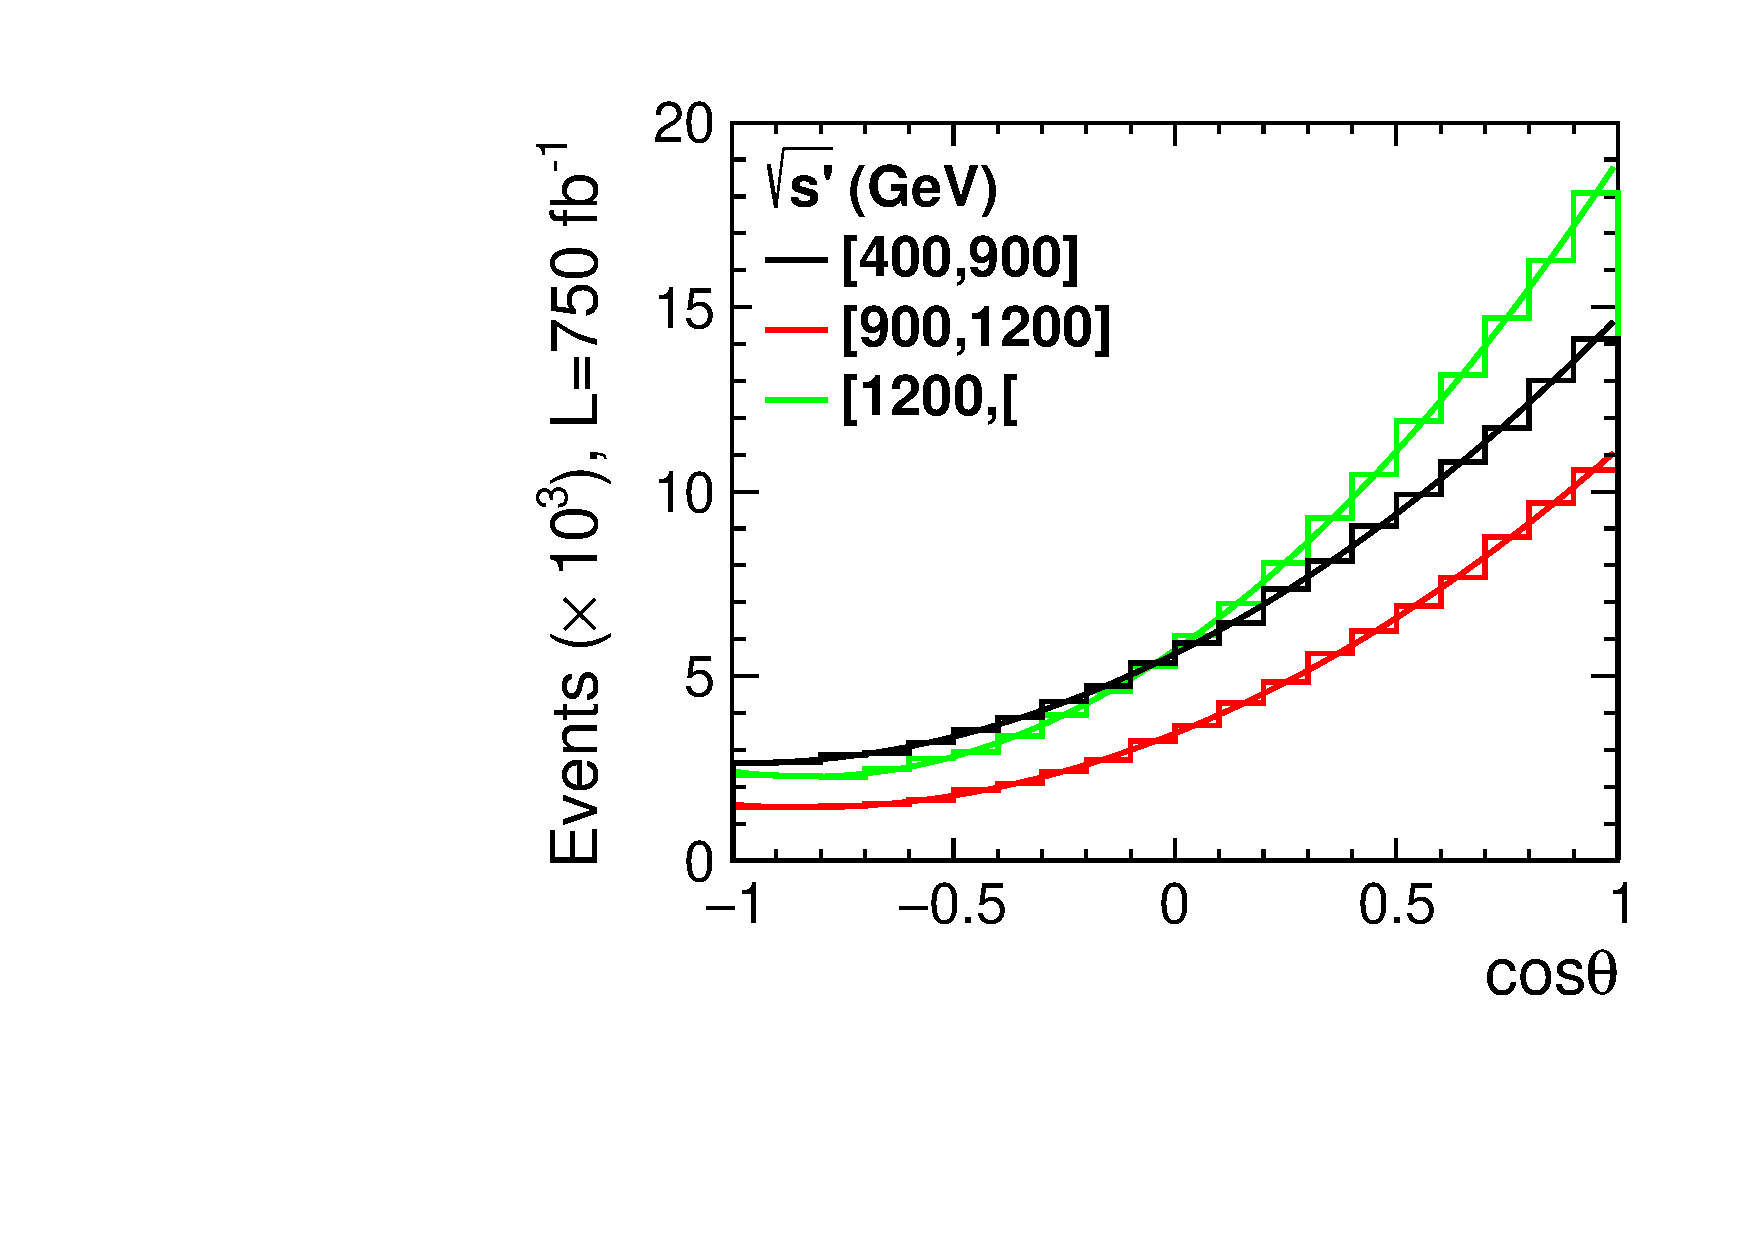
\includegraphics[width=0.6\textwidth]{TopAnalysis/figures/GeneratorTheta.pdf}
  \caption[Generator level $\cos\theta$ distributions for each energy bin]{Generator level $\cos\theta$ distributions for each energy bin for -80\% polarization with fit to \refeq{eq:afbfit}}
  \label{fig:mctheta}
\end{figure}

The expected $\cos\theta$ distributions at generator level are shown in \reffig{fig:mctheta} along with their fits to \refeq{eq:afbfit} for $-$80\% electron polarization operation. The precision that can be expected using the fit and the simpler method for each energy assuming perfect event reconstruction is shown in \reftab{table:idealresults}. In all cases $\cos\theta$ is measured in the $t\bar{t}$ rest frame. To increase the number of available signal events, $\cos\theta$ is multiplied by the charge of the lepton so that events in which it is the antitop that decays hadronically the angle of the top can still be recovered. Note that this is only possible when measuring $A_{FB}^t$ in the $t\bar{t}$ rest frame where the top and antitop are produced back to back.

\begin{table}
  \centering
  \begin{tabular}{l|c|c|c|c|c}
    \toprule
    Energy (GeV) &  $\sigma$ (fb)   & $A_{FB}^t$ & $\Delta A^t_{FB}$ (Counting) & $\Delta A_{FB}^t$ (Fit) \\
    \midrule
    $>=$1200 & 18.4  & 0.563 & 0.007 & 0.006 \\
    \midrule
    900-1200 & 11.0 & 0.547 & 0.009 & 0.008 \\
    \midrule
    400-900 & 16.6 & 0.457 & 0.008 & 0.007 \\
    \bottomrule
  \end{tabular}
  \caption{Precision attainable on $A_{FB}^t$ during the -80\% electron polarization stage assuming perfect event reconstruction for the simple counting method vs the fit method for extraction}
  \label{table:idealresults}
\end{table}


\section{Event Selection}
\label{Event Selection}

Event selection is performed in three distinct stages: preselection, quality cuts and \ac{BDT} selection, with each stage having its own purpose. The preselection is designed to remove easily identifiable backgrounds with minimal reduction in the signal efficiency. Quality cuts are then applied to remove events in which the event reconstruction has failed such as when the fat jets have been incorrectly associated with the hadronically decaying top or lone b jet. The final selection is then performed using a pair of \ac{BDT}s for each polarization that are trained to identify low and high energy signal events and reject any remaining backgrounds. The preselection cuts, quality cuts and choice of variables used by the \ac{BDT}s were all optimized for the $-$80\% electron polarization state integrated across the full energy range. As such there is likely still some improvement that could be made by individually reoptimising the cuts and variables used for each energy bin and each polarization state but this is not examined here.

\subsection{Preselection}

The preselection cuts were designed to remove easily identifiable backgrounds without a significant reduction in the signal yield. The cuts used were as follows:

\begin{itemize}
\item One charged isolated lepton found
\item Visible transverse momentum $>$ 200 GeV
\item Energy of the hadronically decaying top $>$ 100 GeV
\item Transverse momentum of the lone b jet $>$ 20 GeV
\item -ln$(y_{23})$, $<$ 7, where $y_{23}$ is the jet resolution parameter at the transition from 2 to 3 jets,
\item -ln$(y_{34}) <$ 9
\item $|\cos\theta|$ of the reconstructed top in the lab frame $<$ 0.9
\end{itemize}

The resulting efficiency for the signal and background processes are shown in \reftabs{table:toppreselneg} and \ref{table:toppreselpos}. Clearly there is minimal loss of signal events while certain backgrounds can be suppressed by $\mathcal{O}$(10$^2$).

\begin{table}
  \centering
  \begin{tabular}{l | c | c }
    \toprule
    Process     & Cross Section(fb) & Efficiency  \\
     \midrule
     $e^+e^-\rightarrow t\bar{t} \rightarrow qqqql\nu (l=e,\mu)$& 46.8 & 9.67E-1 \\
    \midrule
    $e^+e^-\rightarrow t\bar{t} \rightarrow qqqql\nu (l=\tau)$& 23.2 & 8.08E-1 \\
    \midrule
    $e^+e^-\rightarrow t\bar{t} \rightarrow qqqql\nu (non ~ t\bar{t})$& 72.3 & 8.22E-1\\
    \midrule
    $e^+e^-\rightarrow qqqqqq$ & 116.4 &  7.56E-1\\
    \midrule
    $e^+e^-\rightarrow qql\nu l\nu$ & 44.1 &  7.55E-1\\
    \midrule
    $e^+e^-\rightarrow qqqq$ & 2304.0 &  2.75E-1\\
    \midrule
    $e^+e^-\rightarrow qql\nu$ & 6975.0 &  1.69E-1\\
    \midrule
    $e^+e^-\rightarrow qqll$ & 2681.0 &  6.45E-2\\
    \midrule
    $e^+e^-\rightarrow qq\nu\nu$ & 1395.0 &  6.85E-2\\
    \midrule
    $e^+e^-\rightarrow qq$ & 4843.0 & 8.61E-2\\
    \bottomrule
  \end{tabular}
  \caption{Efficiency for signal and background processes following pre-selection cuts for -80\% polarization.}
  \label{table:toppreselneg}
\end{table}

\begin{table}
  \centering
  \begin{tabular}{l | c | c }
    \toprule
    Process     & Cross Section(fb) & Efficiency \\
    \midrule
     $e^+e^-\rightarrow t\bar{t} \rightarrow qqqql\nu (l=e,\mu)$& 24.7 & 9.71E-1\\
    \midrule
    $e^+e^-\rightarrow t\bar{t} \rightarrow qqqql\nu (l=\tau)$& 12.3 & 8.15E-1\\
    \midrule
    $e^+e^-\rightarrow t\bar{t} \rightarrow qqqql\nu (non ~ t\bar{t})$& 16.5 & 8.07E-1\\
    \midrule
    $e^+e^-\rightarrow qqqqqq$ & 44.9 &  7.54E-1\\
    \midrule
    $e^+e^-\rightarrow qql\nu l\nu$ & 15.3  & 7.87E-1\\
    \midrule
    $e^+e^-\rightarrow qqqq$ & 347 &  3.07E-1\\
    \midrule
    $e^+e^-\rightarrow qql\nu$ & 1640 &  1.17E-1\\
    \midrule
    $e^+e^-\rightarrow qqll$ & 2530 &  5.21E-2\\
    \midrule
    $e^+e^-\rightarrow qq\nu\nu$ & 180 & 7.30E-2 \\
    \midrule
    $e^+e^-\rightarrow qq$ & 3170 & 6.03E-2 \\
    \bottomrule
  \end{tabular}
  \caption{Efficiency for signal and background processes following pre-selection cuts for +80\% polarization.}
  \label{table:toppreselpos}
\end{table}

\subsection{Quality Cuts}
\label{Quality Cuts}

The quality cuts were designed to remove events in which the reconstruction has failed to reconstruct the top or has assigned the wrong fat jet to be the hadronic top. Doing this helps reduce the migration effects discussed in \refsec{sec:jetassociation} which result in a poor correlation between the reconstructed and generator $\cos\theta$ distributions. As such, the cuts were optimized to reject events in which $|\cos\theta_{Reco}-\cos\theta_{Gen}| > $ 0.05. The optimum cuts found were as follows:

\begin{itemize}
\item Reconstructed hadronically decaying top mass $>$ 100 GeV
\item Mass of the b jet from the leptonically decaying top $<$ 100 GeV
\item P$_T$ of the hadronically decaying top $>$ 100 GeV
\item 0.2 $< \cos\theta_{12} <$ 0.9, where $\theta_{12}$ is the angle between the two highest energy subjets of the three subjets in the hadronic fat jet (See \refsec{subjAngular})
\item $y_{23} <$ 3
\item $\mid$ Total P$_z \mid <$ 100 GeV
\end{itemize}

For reasons discussed later in \refsec{sec:topsystematics} relating to minimizing biases, an additional cut on the momentum of the isolated lepton $>$ 70 GeV is also included for the lowest energy bin. As already noted, some improvement in the performance could be achieved by separately optimizing the cuts for each energy bin and polarization. This is particularly true for variables such as $\cos\theta_{12}$ which are not Lorentz invariant and so will remove more signal events in the lower energy bins than the higher ones, however no Lorentz invariant equivalents to these cuts were found to provide as reliable discrimination against poorly reconstructed events. That being said, the efficiency is expected to be lower for the lower energy bins regardless as the jet reconstruction has already been shown to be less reliable for lower $\sqrt{s'}$ events and so the jets are less likely to have the correct kinematic properties of the generator level tops, i.e. the ratio  $\frac{|\cos\theta_{Reco-Gen}| > X}{|\cos\theta_{Reco-Gen}| < X}$ will always be higher in the lower energy bins. Again this motivates an additional future study dedicated to reconstructing events in the lowest energy bin.

The resulting efficiency for the signal and background processes following the preselection and quality cuts are shown in \reftabs{table:topqualneg} and \ref{table:topqualpos}.

\begin{table}
  \centering
  \begin{tabular}{l | c | c }
    \toprule
    Process     & Cross Section(fb) & Efficiency  \\
    \midrule
    $e^+e^-\rightarrow t\bar{t} \rightarrow qqqql\nu (l=e,\mu)$&  &  \\
    E$>=$1200 GeV & 18.4 & 3.67E-1 \\
    900$<=$E$<$1200 GeV & 11.0 & 3.33E-1 \\
    400$<=$E$<$900 GeV & 16.6 & 4.00E-2 \\
    \midrule
    $e^+e^-\rightarrow t\bar{t} \rightarrow qqqql\nu (l=\tau)$& 23.2 & 2.52E-1 \\
    \midrule
    $e^+e^-\rightarrow t\bar{t} \rightarrow qqqql\nu (non ~ t\bar{t})$& 72.3 & 9.82E-2\\
    \midrule
    $e^+e^-\rightarrow qqqqqq$ & 116.4 & 5.86E-2  \\
    \midrule
    $e^+e^-\rightarrow qql\nu l\nu$ & 44.1 & 5.25E-2 \\
    \midrule
    $e^+e^-\rightarrow qqqq$ & 2304.0 & 1.07E-2 \\
    \midrule
    $e^+e^-\rightarrow qql\nu$ & 6975.0 & 1.08E-3 \\
    \midrule
    $e^+e^-\rightarrow qqll$ & 2681.0 & 8.32E-4 \\
    \midrule
    $e^+e^-\rightarrow qq\nu\nu$ & 1395.0 & 1.77E-4 \\
    \midrule
    $e^+e^-\rightarrow qq$ & 4843.0 & 6.93E-3\\
    \bottomrule
  \end{tabular}
  \caption{Efficiency for signal and background processes following pre-selection and quality cuts for -80\% polarization.}
  \label{table:topqualneg}
\end{table}

\begin{table}
  \centering
  \begin{tabular}{l | c | c }
    \toprule
    Process     & Cross Section(fb) & Efficiency \\
    \midrule
    $e^+e^-\rightarrow t\bar{t} \rightarrow qqqql\nu (l=e,\mu)$&  &  \\
    E$>=$1200 GeV & 9.84 & 3.45E-1 \\
    900$<=$E$<$1200 GeV & 5.79 & 3.02E-1 \\
    400$<=$E$<$900 GeV & 8.7 & 5.00E-2 \\
    \midrule
    $e^+e^-\rightarrow t\bar{t} \rightarrow qqqql\nu (l=\tau)$& 12.3 & 2.52E-1\\
    \midrule
    $e^+e^-\rightarrow t\bar{t} \rightarrow qqqql\nu (non ~ t\bar{t})$& 16.5 & 1.48E-1\\
    \midrule
    $e^+e^-\rightarrow qqqqqq$ & 44.9 & 6.01E-2 \\
    \midrule
    $e^+e^-\rightarrow qql\nu l\nu$ & 15.3  & 8.77E-2 \\
    \midrule
    $e^+e^-\rightarrow qqqq$ & 347 & 1.64E-2 \\
    \midrule
    $e^+e^-\rightarrow qql\nu$ & 1640 & 5.87E-4 \\
    \midrule
    $e^+e^-\rightarrow qqll$ & 2530 & 6.15E-4 \\
    \midrule
    $e^+e^-\rightarrow qq\nu\nu$ & 180 & 3.01E-4 \\
    \midrule
    $e^+e^-\rightarrow qq$ & 3170 & 4.80E-3 \\
    \bottomrule
  \end{tabular}
  \caption{Efficiency for signal and background processes following pre-selection and quality cuts for +80\% polarization.}
  \label{table:topqualpos}
\end{table}

This step is where the largest loss in signal efficiency occurs during the selection process. While this is undesirable, one can see from \reffig{fig:qualitycuts} that the quality selection does provide a vast improvement in the agreement between the reconstructed and generator level $\cos\theta$ distributions. This is desirable as it reduces the chance of a bias being introduced in $A_{FB}^t$ from the misreconstruction of events. A discussion of possible remaining biases from this is presented in \refsec{sec:topsystematics}. 

\begin{figure}
  \centering
  \begin{subfigure}{.5\textwidth}
    \centering
    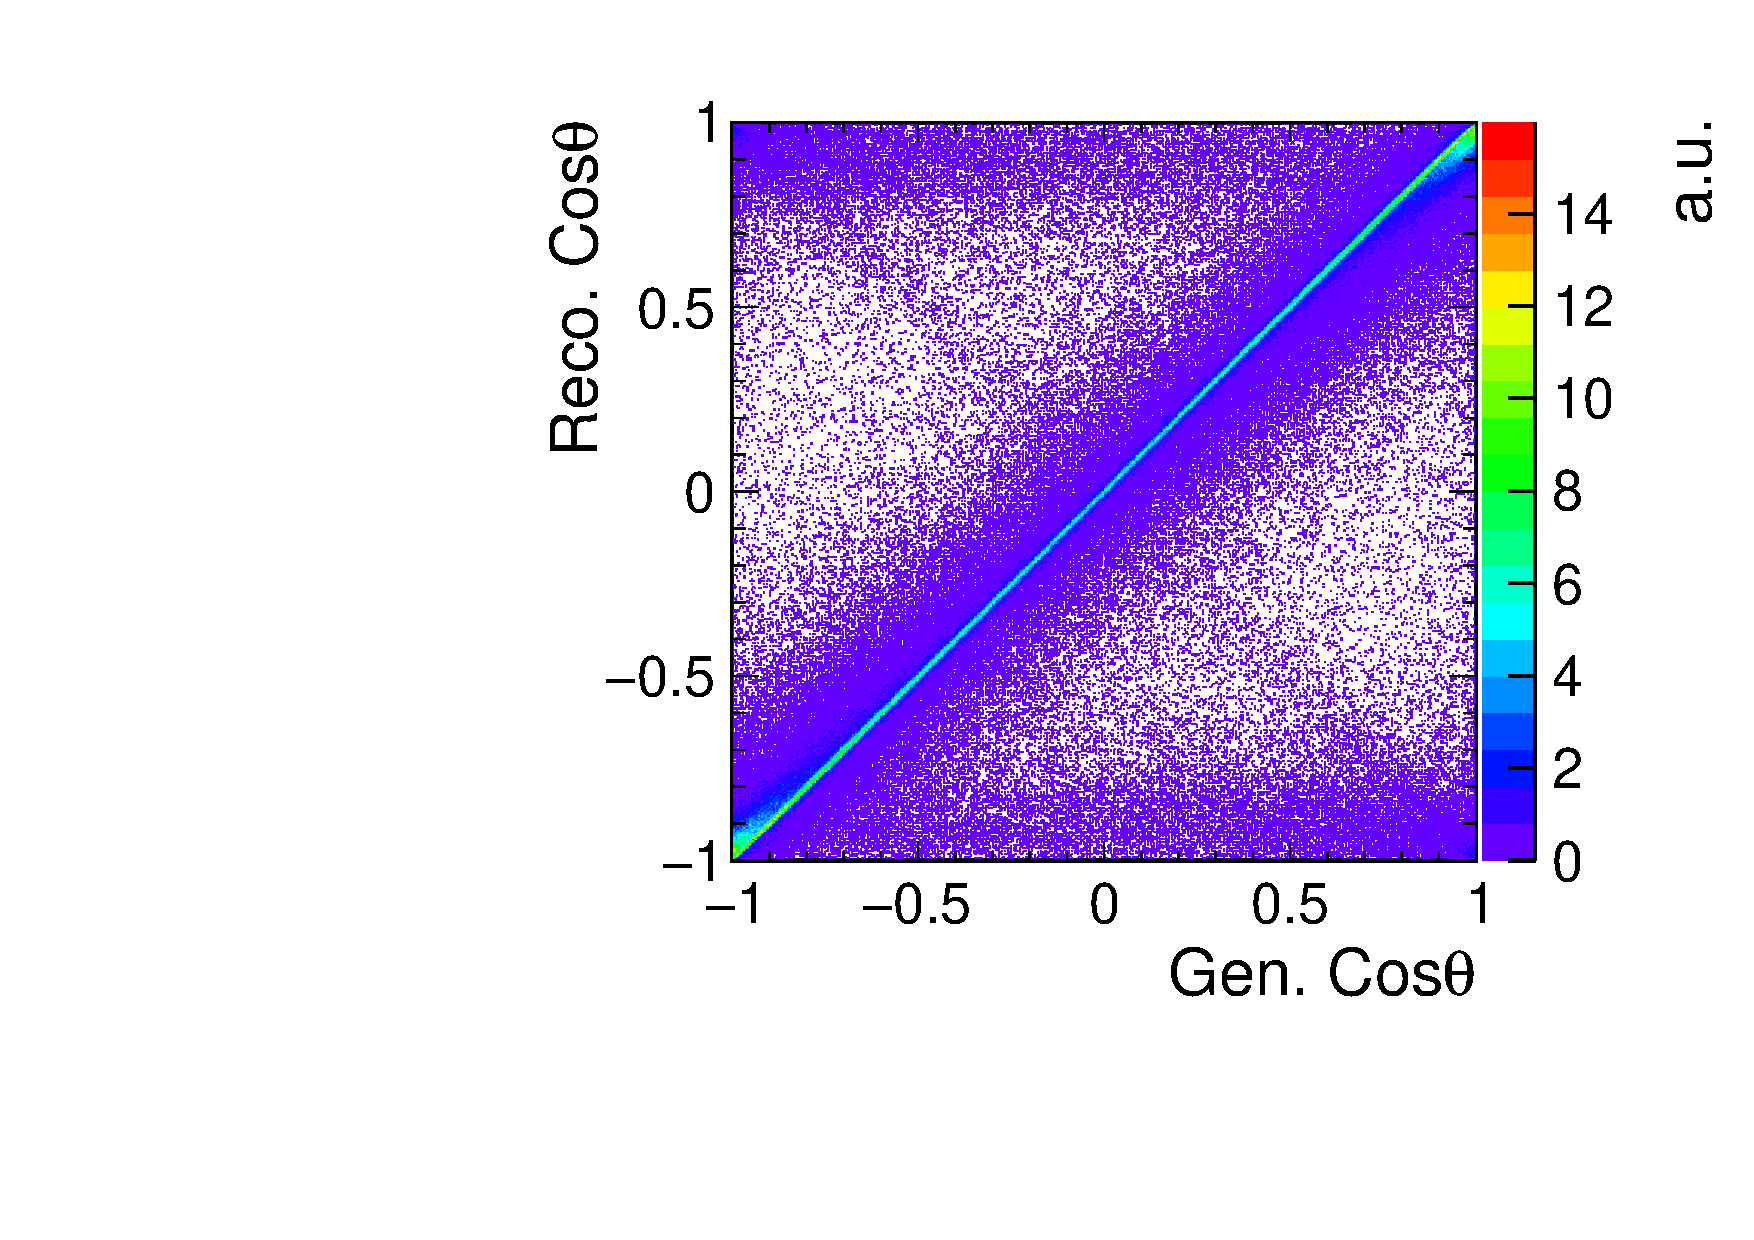
\includegraphics[width=0.9\textwidth]{TopAnalysis/figures/CosThetaRecoVsMC.pdf}
    \caption{Before Quality Selection}
  \end{subfigure}%
  \begin{subfigure}{.5\textwidth}
    \centering
    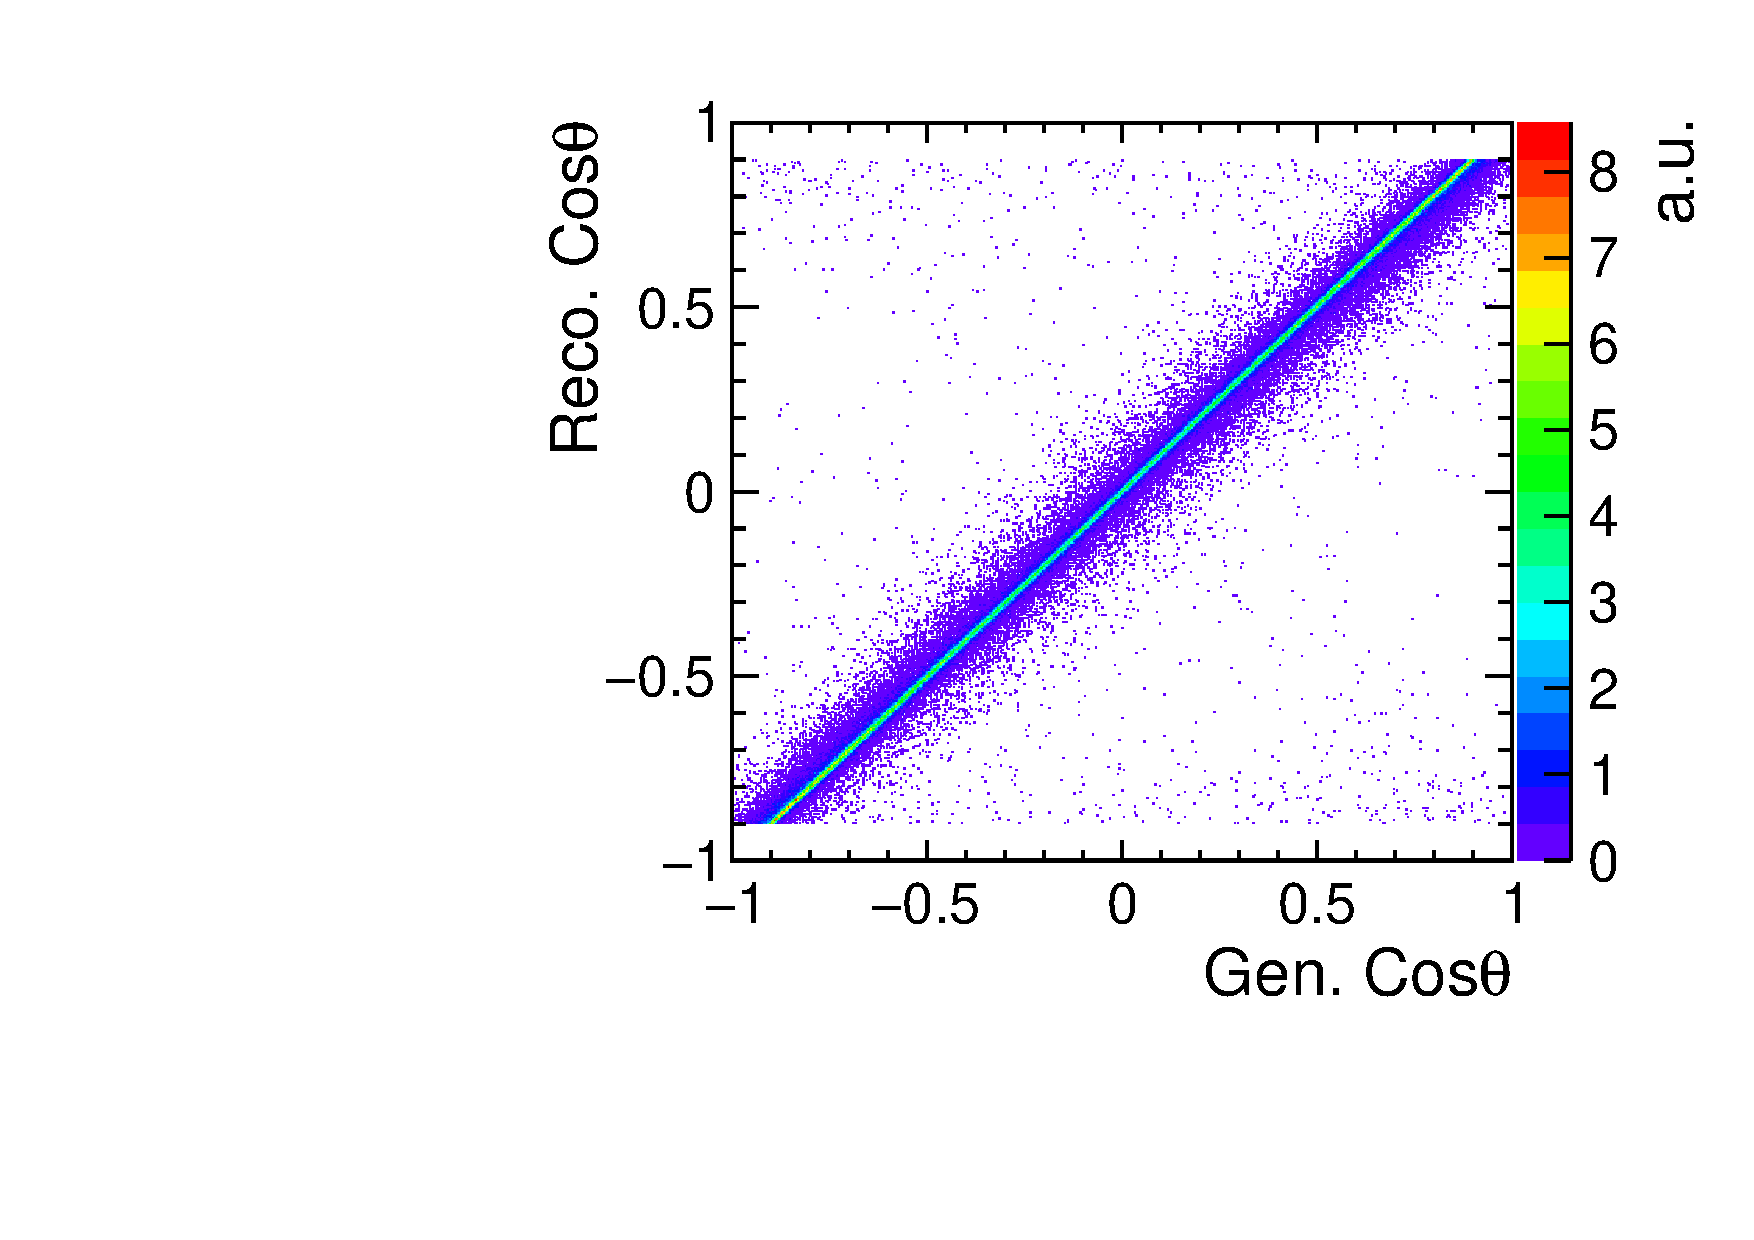
\includegraphics[width=0.9\textwidth]{TopAnalysis/figures/CosThetaRecoVsMC_QualityCuts.pdf}
    \caption{After Quality Selection}
  \end{subfigure}
  \caption[Effect of quality selection on agreement of $\cos\theta$ reco. vs gen.]{Effect of quality selection on agreement of $\cos\theta$ reco. vs gen.}
  \label{fig:qualitycuts}
\end{figure}


\subsection{BDT Selection}

The final stage of selection uses a multivariate approach to remove any remaining backgrounds. Two \ac{BDT}s were trained for each polarization state where one is trained on events with generator $\sqrt{s'} >=$ 1.2 TeV and the other is trained on events with  $\sqrt{s'} <$ 1.2 TeV. The selection itself is performed by placing a cut on the score from each \ac{BDT} and selecting events which pass either cut in each energy bin. The choice of cut on each score is optimized for each energy bin in order to maximize the statistical significance, $S/\sqrt{S+B}$. This helps to improve the performance due to the fact the signal topology is quite different in the two energy regions due to the different boost factors. If only one \ac{BDT} was used it would have to simultaneously identify events with both topologies making it harder to identify background events. With two \ac{BDT}s, the high energy \ac{BDT} is more capable of rejecting backgrounds with a topology similar to the low energy signal and vice versa. To further improve the \ac{BDT} performance, only 6 fermion, qq and qqlv final states were included in the training as these are the most challenging to remove.  Negligible amounts of other event were found to pass the \ac{BDT} despite not specifically being trained against. In all cases the BDT is trained on the 21 variables listed below. The mass of the reconstructed top is deliberately not included to prevent a possible bias towards the generator top mass. For each \ac{BDT}, the relevant samples are split evenly between training and testing. In order to make optimal use of the limited samples available, for each \ac{BDT} an additional \ac{BDT} is trained in which the samples are reversed so that all events can be used for training and for testing. Care is taken to ensure that no event trains and is tested by the same \ac{BDT}.

\begin{itemize}
\item Total visible energy and transverse momentum
\item Centre-of-mass of the event
\item Energy and transverse momentum of hadronic fat jet
\item Mass, $\tau_1$ and $\tau_2/\tau_1$ of leptonic fat jet
\item Relative angles of the three subjets within the hadronic fat jet
\item Energy, transverse momentum and total momentum of the isolated lepton
\item Number of lepton candidates with energy $>$ 30 GeV
\item Angular separation of the lepton and hadronic fat jet
\item -ln(y$_{23}$)
\item Thrust major of the event
\item Energy of the leptonically decaying top
\item Highest and next to highest btags
\end{itemize}

The resulting distributions of the \ac{BDT} scores for each classifier are shown in \reffig{fig:topbdtscores}. A high degree of separation is seen in all cases, though it is more pronounced in the higher energy classifiers. The efficiencies and expected number of events after 750 fb$^{-1}$ are shown for the high energy bins only in \reftabs{table:topfinalefficienciesneg} and \ref{table:topfinalefficienciespos}. The equivalent results for the lower energy bins can be found in Appendix B along with the distributions for each of the variables used for training the \ac{BDT}. Overall it can be seen that a good signal to background ratio is achieved for a moderate signal efficiency in the higher energy bins. The background is dominated by 6 fermion final states, predominantly from $t\bar{t}$ and single top events as expected. Further improvements might be made if tau tagging was possible, however as already discussed in the previous chapter, an adequately performant tau finder has yet to be developed for \ac{CLIC}. 

\begin{figure}[ht] 
  \begin{subfigure}[b]{0.5\linewidth}
    \centering
    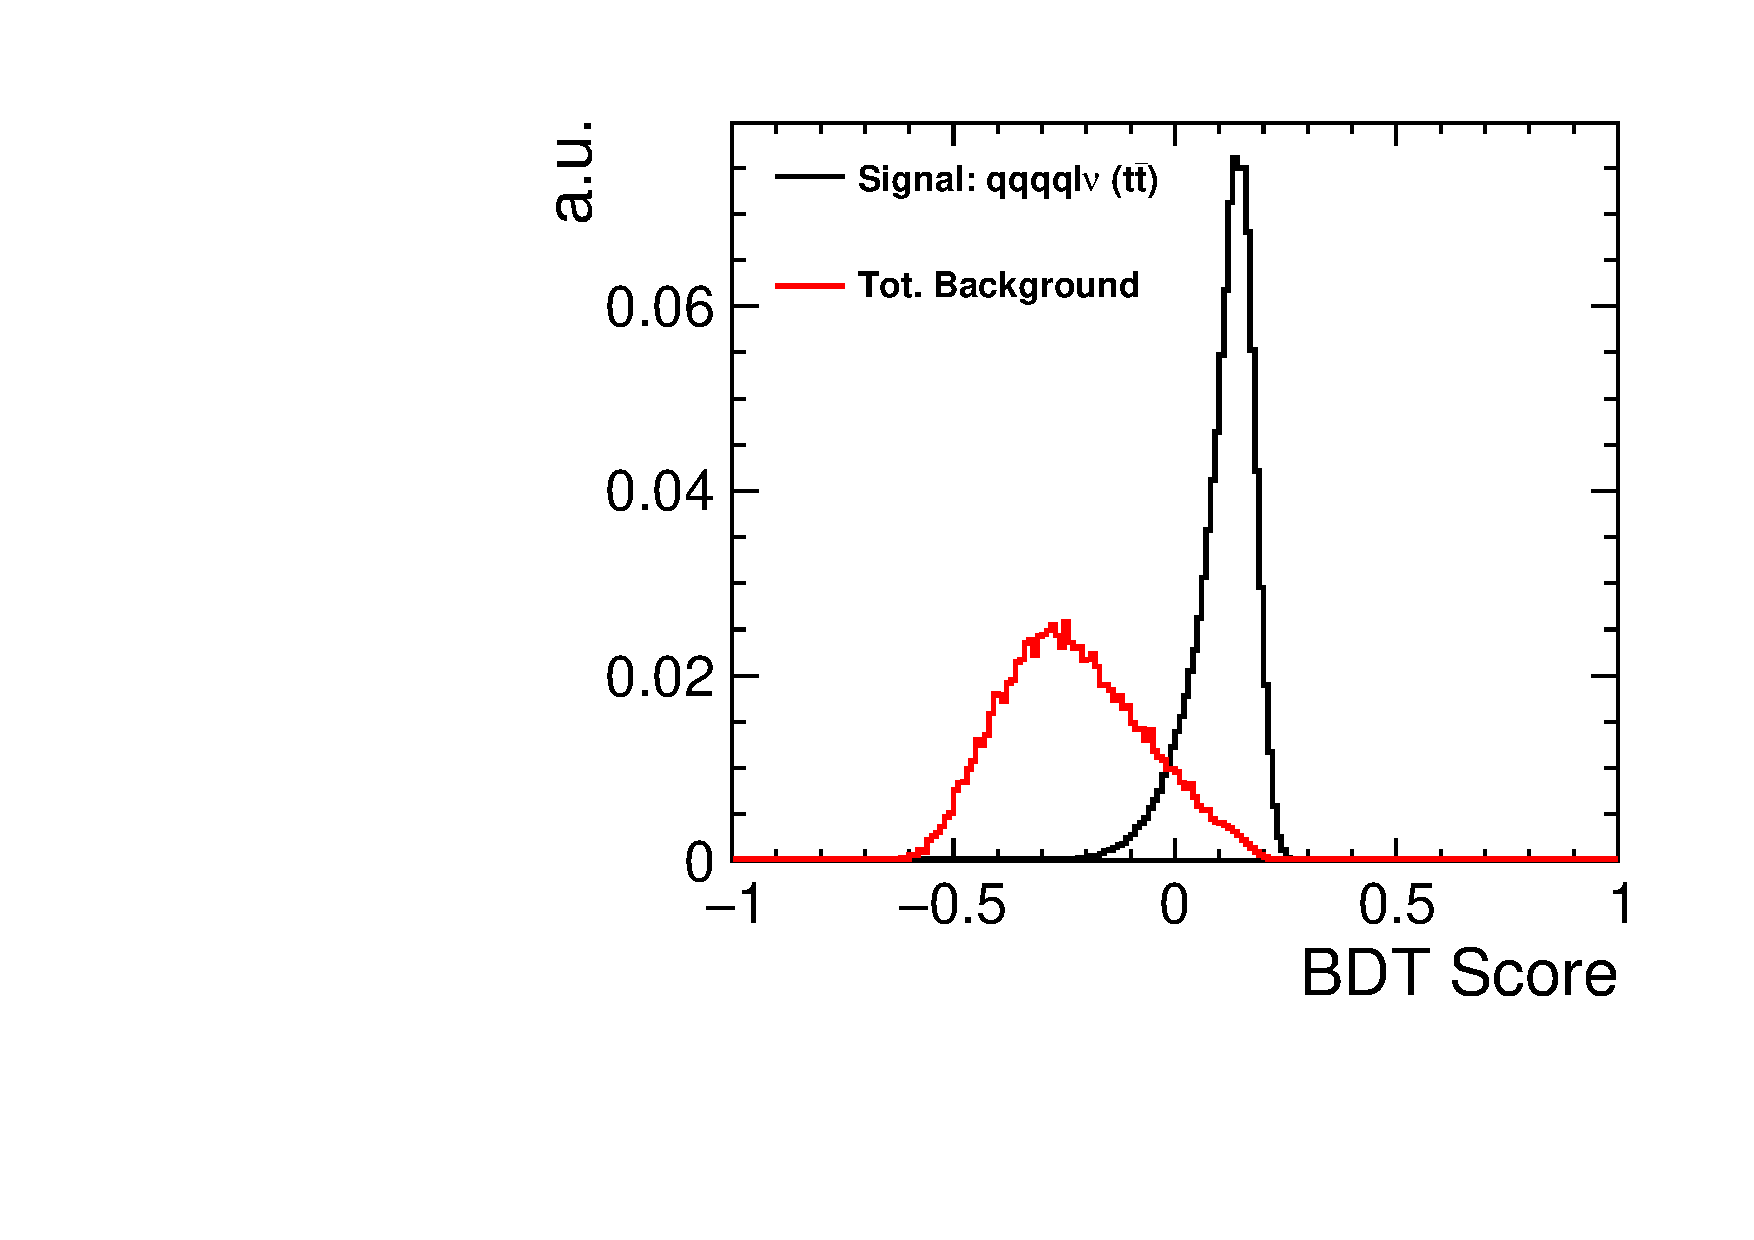
\includegraphics[width=0.99\linewidth]{TopAnalysis/figures/BDTScoreHighENeg.pdf} 
    \caption{High energy, -80\% polarization} 
    \vspace{4ex}
  \end{subfigure}%% 
  \begin{subfigure}[b]{0.5\linewidth}
    \centering
    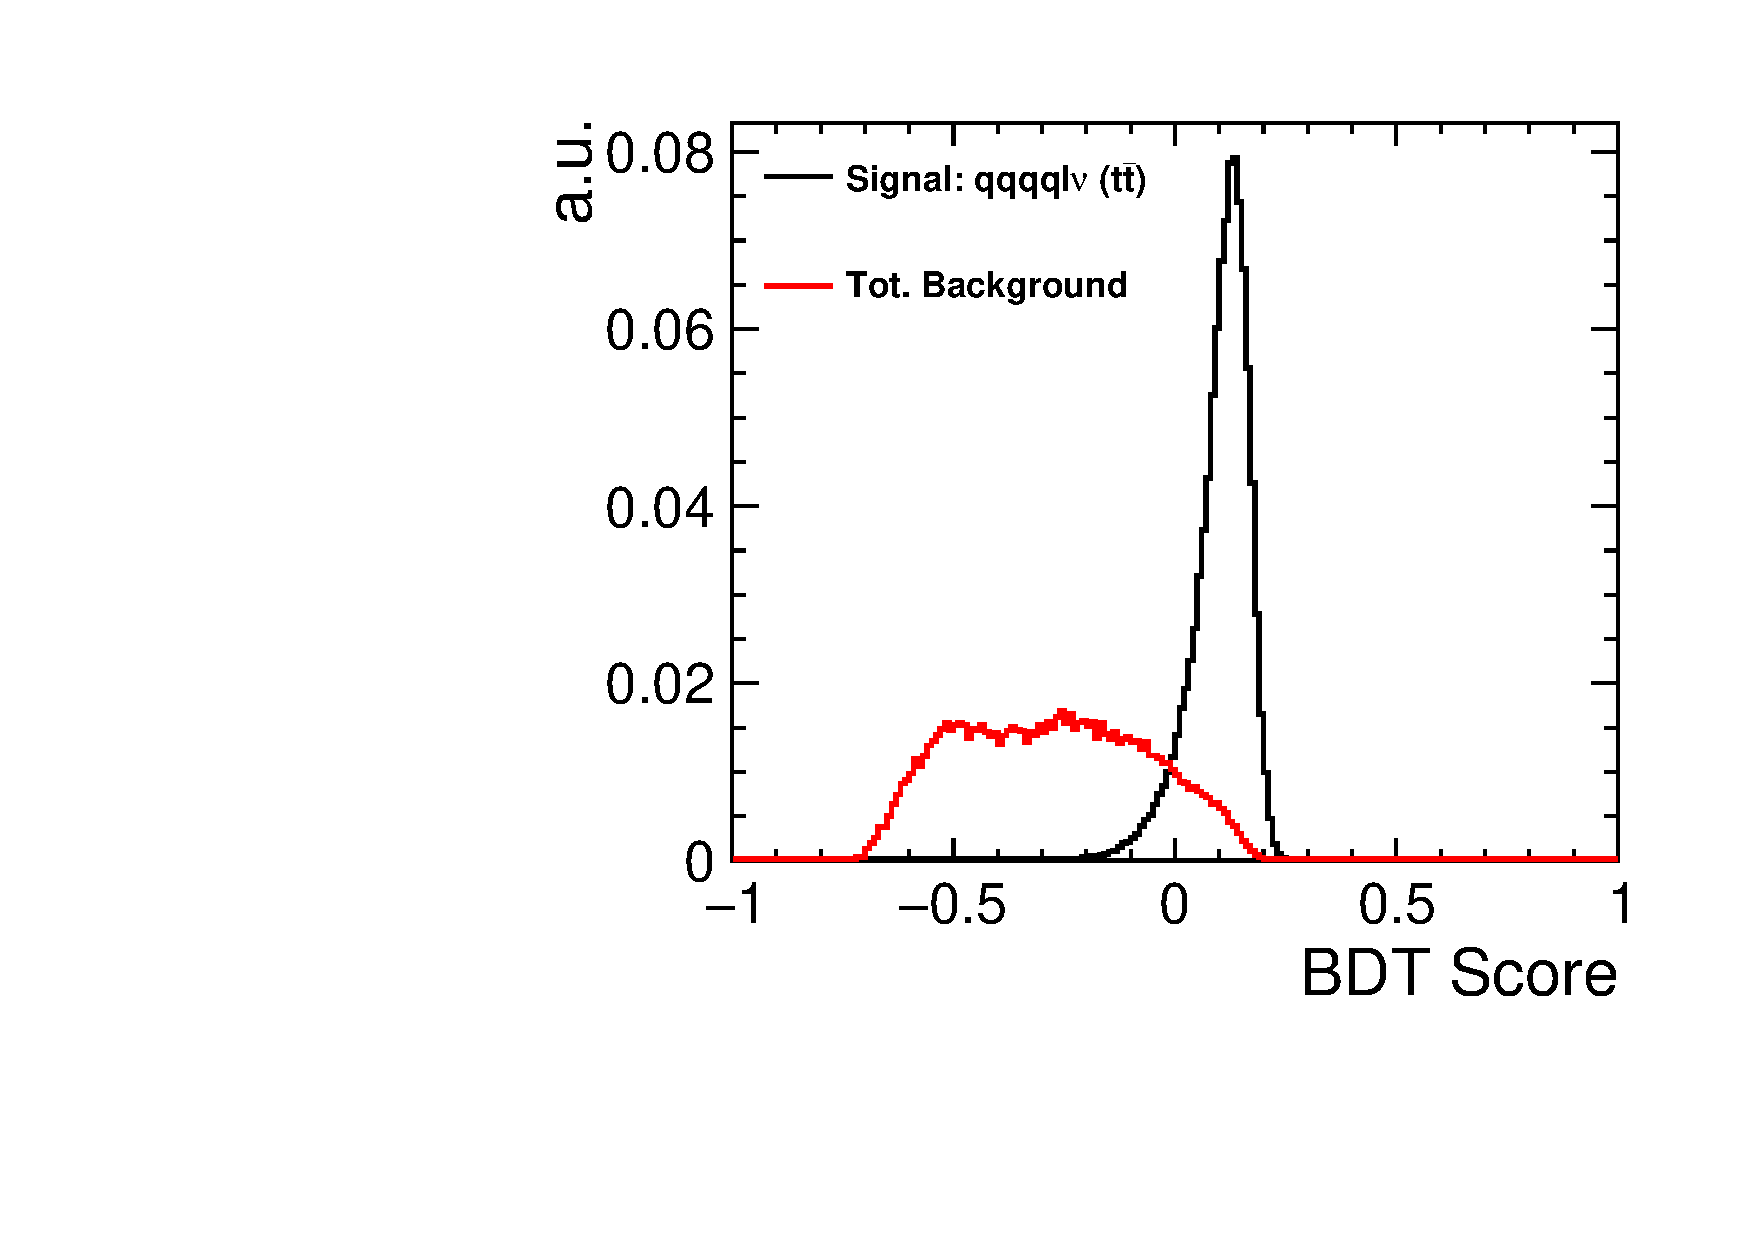
\includegraphics[width=0.99\linewidth]{TopAnalysis/figures/BDTScoreLowENeg.pdf} 
    \caption{Low energy, -80\% polarization} 
    \vspace{4ex}
  \end{subfigure} 
\end{figure}

\begin{figure}[ht]\ContinuedFloat 
  \begin{subfigure}[b]{0.5\linewidth}
    \centering
    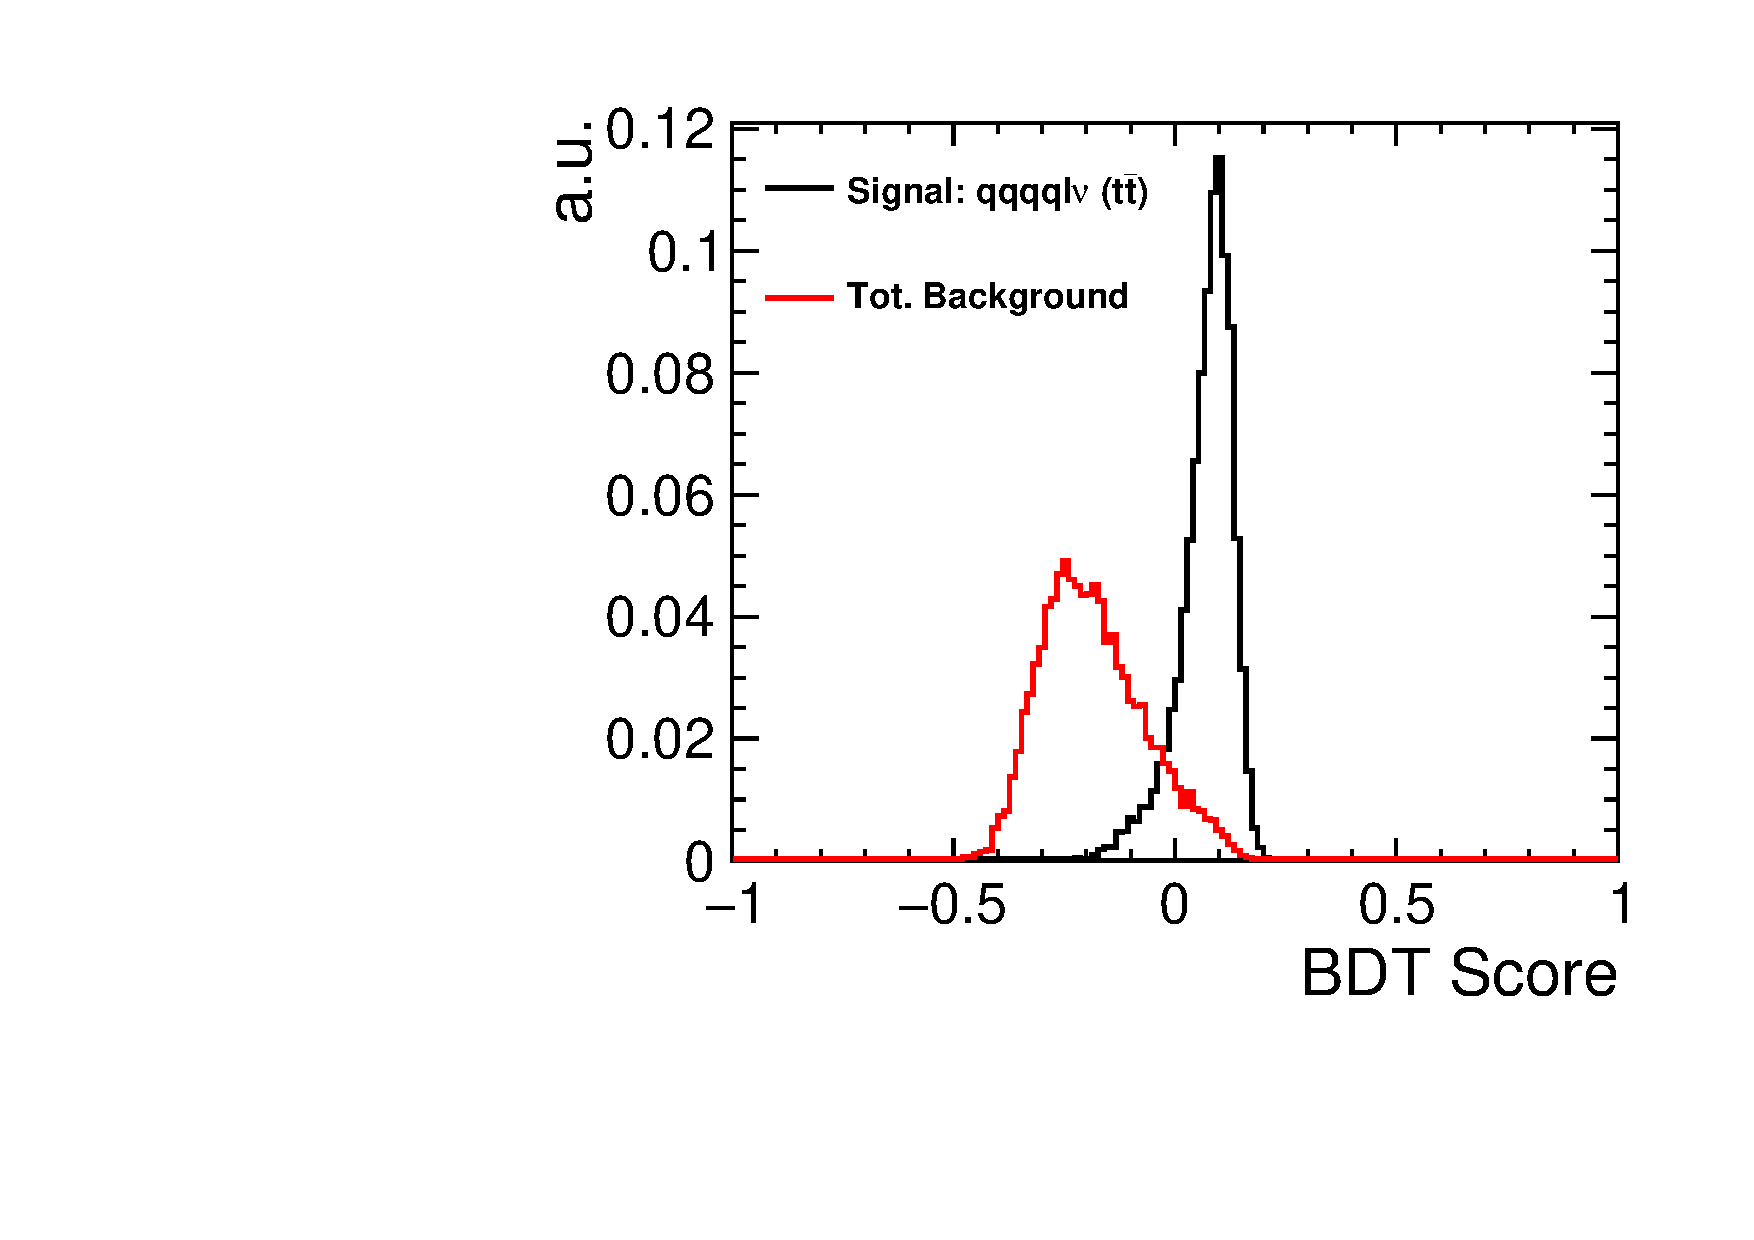
\includegraphics[width=0.99\linewidth]{TopAnalysis/figures/BDTScoreHighEPos.pdf} 
    \caption{High energy, +80\% polarization} 
    \vspace{4ex}
  \end{subfigure}%% 
  \begin{subfigure}[b]{0.5\linewidth}
    \centering
    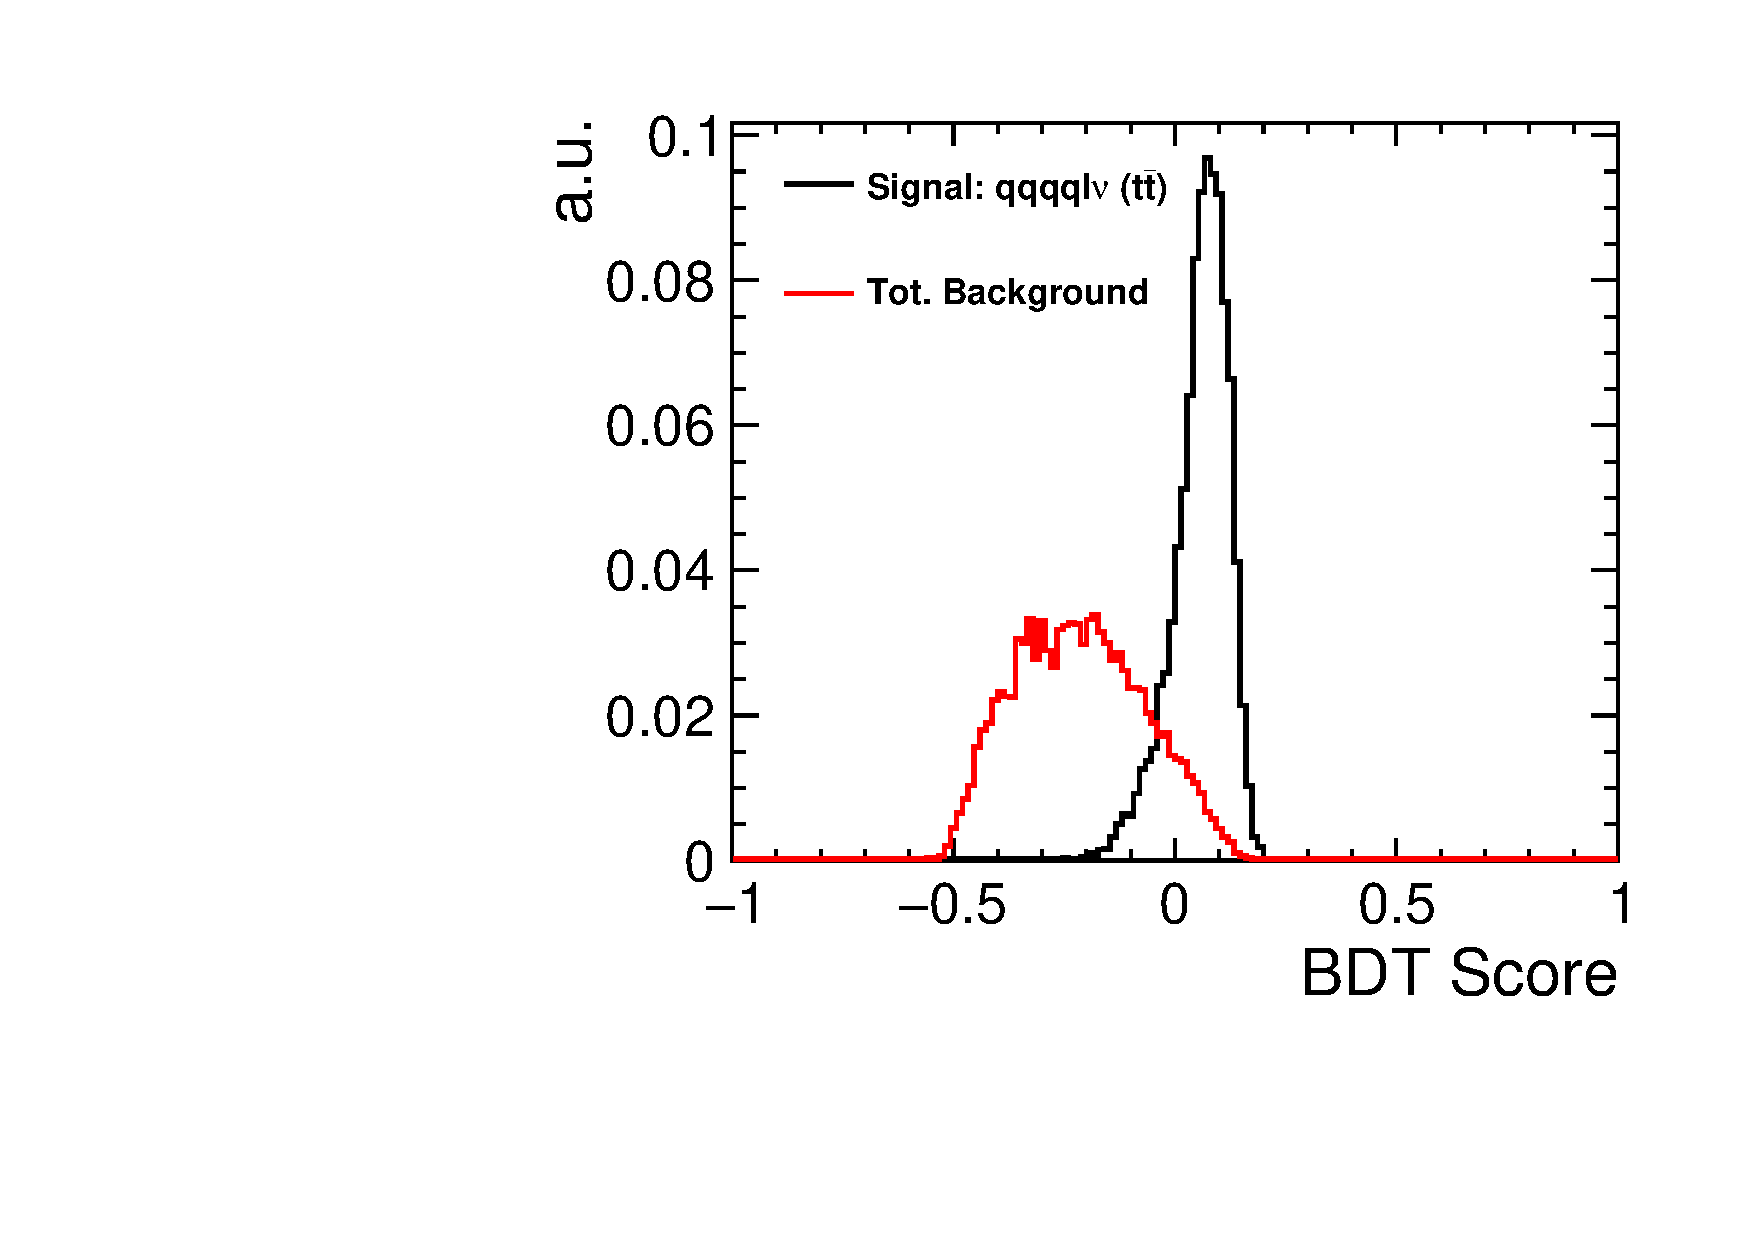
\includegraphics[width=0.99\linewidth]{TopAnalysis/figures/BDTScoreLowEPos.pdf} 
    \caption{Low energy, +80\% polarization} 
    \vspace{4ex}
  \end{subfigure}
  \caption[\ac{BDT} performance for all four classifiers]{\ac{BDT} performance for all four classifiers. Signal: $qqqql\nu (t\bar{t})$ is shown in black, background is shown in red.}
  \label{fig:topbdtscores}
\end{figure}

\begin{table}
  \centering
  \begin{tabular}{l | c | c | c | c}
    \toprule
     Process     & Cross Section & Efficiency & Efficiency & N Expected\\
     & (fb) & Pre. \& Quality & BDT & \\
     \midrule
    $e^+e^-\rightarrow t\bar{t} \rightarrow qqqql\nu (l=e,\mu)$&  &  & &\\
     E$>=$1200 GeV & 18.4 & 3.67E-1 & 3.15E-1 & 4350\\
     E$<$1200 GeV & 28.4 & 3.11E-2 & 2.59E-2 & 550 \\
    \midrule
    $e^+e^-\rightarrow t\bar{t} \rightarrow qqqql\nu (l=\tau)$& 23.2 & 1.20E-1 & 3.67E-2 & 640 \\
    \midrule
    $e^+e^-\rightarrow t\bar{t} \rightarrow qqqql\nu (non ~ t\bar{t})$& 72.3 & 4.80E-2 & 2.27E-2 & 1230\\
    \midrule
    $e^+e^-\rightarrow qqqqqq$ & 116.4 &  2.23E-2 &1.17E-3 & 100 \\
    \midrule
    $e^+e^-\rightarrow qql\nu l\nu$ & 44.1 & 1.48E-2 & 8.38E-3 & 280\\
    \midrule
    $e^+e^-\rightarrow qqqq$ & 2304.0 & 4.45E-3 & 4.72E-5 & 80 \\
    \midrule
    $e^+e^-\rightarrow qql\nu$ & 6975.0 & 4.75E-4 & 1.04E-5 & 50 \\
    \midrule
    $e^+e^-\rightarrow qqll$ & 2681.0 & 3.10E-4 & 1.19E-5 & 20 \\
    \midrule
    $e^+e^-\rightarrow qq\nu\nu$ & 1395.0 & 6.37E-5 & $<$E-6 & 0 \\
    \midrule
    $e^+e^-\rightarrow qq$ & 4843.0 & 2.97E-3 & 4.83E-5 & 180\\
    \midrule
    \midrule
    Total Background & 18500 & 2.12E-3 & 2.26E-4 & 3140 \\
    \bottomrule
  \end{tabular}
  \caption{Efficiency for signal and background processes being classified as E $>$ 1200 GeV following all stages of selection, and the expected number of events for 750 fb$^{-1}$ for -80\% polarization.}
  \label{table:topfinalefficienciesneg}
\end{table}

\begin{table}
  \centering
  \begin{tabular}{l | c | c | c | c}
    \toprule
    Process     & Cross Section & Efficiency & Efficiency & N Expected\\
         & (fb) & Pre. \& Quality & BDT & \\
    \midrule
    $e^+e^-\rightarrow t\bar{t} \rightarrow qqqql\nu (l=e,\mu)$ &  & \\
    E$>=$1200 GeV & 9.84 & 3.45E-1 & 3.04E-1 & 2240\\
    E$<$1200 GeV & 14.9 & 3.26E-2 & 2.81E-2 & 310 \\
   \midrule
    $e^+e^-\rightarrow t\bar{t} \rightarrow qqqql\nu (l=\tau)$& 12.3 & 1.25E-1 & 3.40E-2 & 310\\
    \midrule
    $e^+e^-\rightarrow t\bar{t} \rightarrow qqqql\nu (non ~ t\bar{t})$& 16.5 & 7.07E-2 & 4.47E-2 & 550\\
    \midrule
    $e^+e^-\rightarrow qqqqqq$ & 44.9 & 2.17E-2 & 1.27E-3 & 40 \\
    \midrule
    $e^+e^-\rightarrow qql\nu l\nu$ & 15.3  & 2.44E-2 & 1.59E-2 & 180 \\
    \midrule
    $e^+e^-\rightarrow qqqq$ & 347.0 & 7.13E-3 & 1.45E-4 & 40 \\
    \midrule
    $e^+e^-\rightarrow qql\nu$ & 1644.0 & 2.56E-4 & 1.59E-5 & 20\\
    \midrule
    $e^+e^-\rightarrow qqll$ & 2529.0 & 2.13E-4 & 1.38E-5 & 30 \\
    \midrule
    $e^+e^-\rightarrow qq\nu\nu$ & 180.0 & 1.16E-4 & $<$E-6 & 0 \\
    \midrule
    $e^+e^-\rightarrow qq$ & 3169.0 & 2.05E-3 & 5.45E-5 & 130 \\
    \midrule
    \midrule
    Total Background & 7970 & 1.82E-3 & 2.71E-4 & 1620\\
    \bottomrule
  \end{tabular}
  \caption{Efficiency for signal and background processes being classified as E $>$ 1200 GeV following all stages of selection and the expected number of events for 750 fb$^{-1}$ for +80\% polarization.}
  \label{table:topfinalefficienciespos}
\end{table}

\section{Extraction of $A_{FB}^t$ and cross section}
As discussed earlier, the measurement of the cross section and $A_{FB}^t$ can be performed simultaneously by fitting to \refeq{eq:afbfit}. However before this can be done, corrections must be made to account for remaining backgrounds and finite efficiencies. In both cases it is assumed that there is no statistical uncertainty introduced in these corrections as the statistical uncertainty can be made arbitrarily small by generating a sufficiently large event sample. Background subtraction was done assuming perfect background modeling in each bin. The uncertainty on the background is instead accounted for later as a systematic effect. After the background has been subtracted, bin by bin efficiency corrections are applied to scale back to the generator distribution. By definition this means that the final distribution the fit is performed on will have the same content per bin as the generator distribution with only the uncertainty on each bin changing. Due to the large statistical sample available for the signal process, the efficiency corrections can be calculated by splitting the signal sample in two, evaluating the efficiency per bin in each sample and scaling by these efficiencies in the alternative sample.

Following these corrections the fit can finally be applied. Due to the fact a cut of $\mid\cos\theta\mid < 0.9$ is applied in the lab frame, the fit is only performed in this same range in the $t\bar{t}$ rest frame as there are a statistically insignificant number of events reconstructed outside this range and so the efficiency corrections are large in these regions. The resulting fits, along with the $\cos\theta$ distributions before the corrections are applied are shown in \reffig{fig:finalfits}. The values for $A_{FB}^t$ and the total cross section along with their uncertainties are extracted from the fit, where the correlated errors between parameters $\sigma_U$ and $\sigma_L$ are taken into account when determining the total cross section uncertainty. These values along with the generator values for $A_{FB}^t$ and $\sigma_{Total}$ are shown for each energy and beam polarization in \reftab{tab:finalfitresults}.


\begin{figure}[] 
  \begin{subfigure}[]{0.5\linewidth}
    \centering
    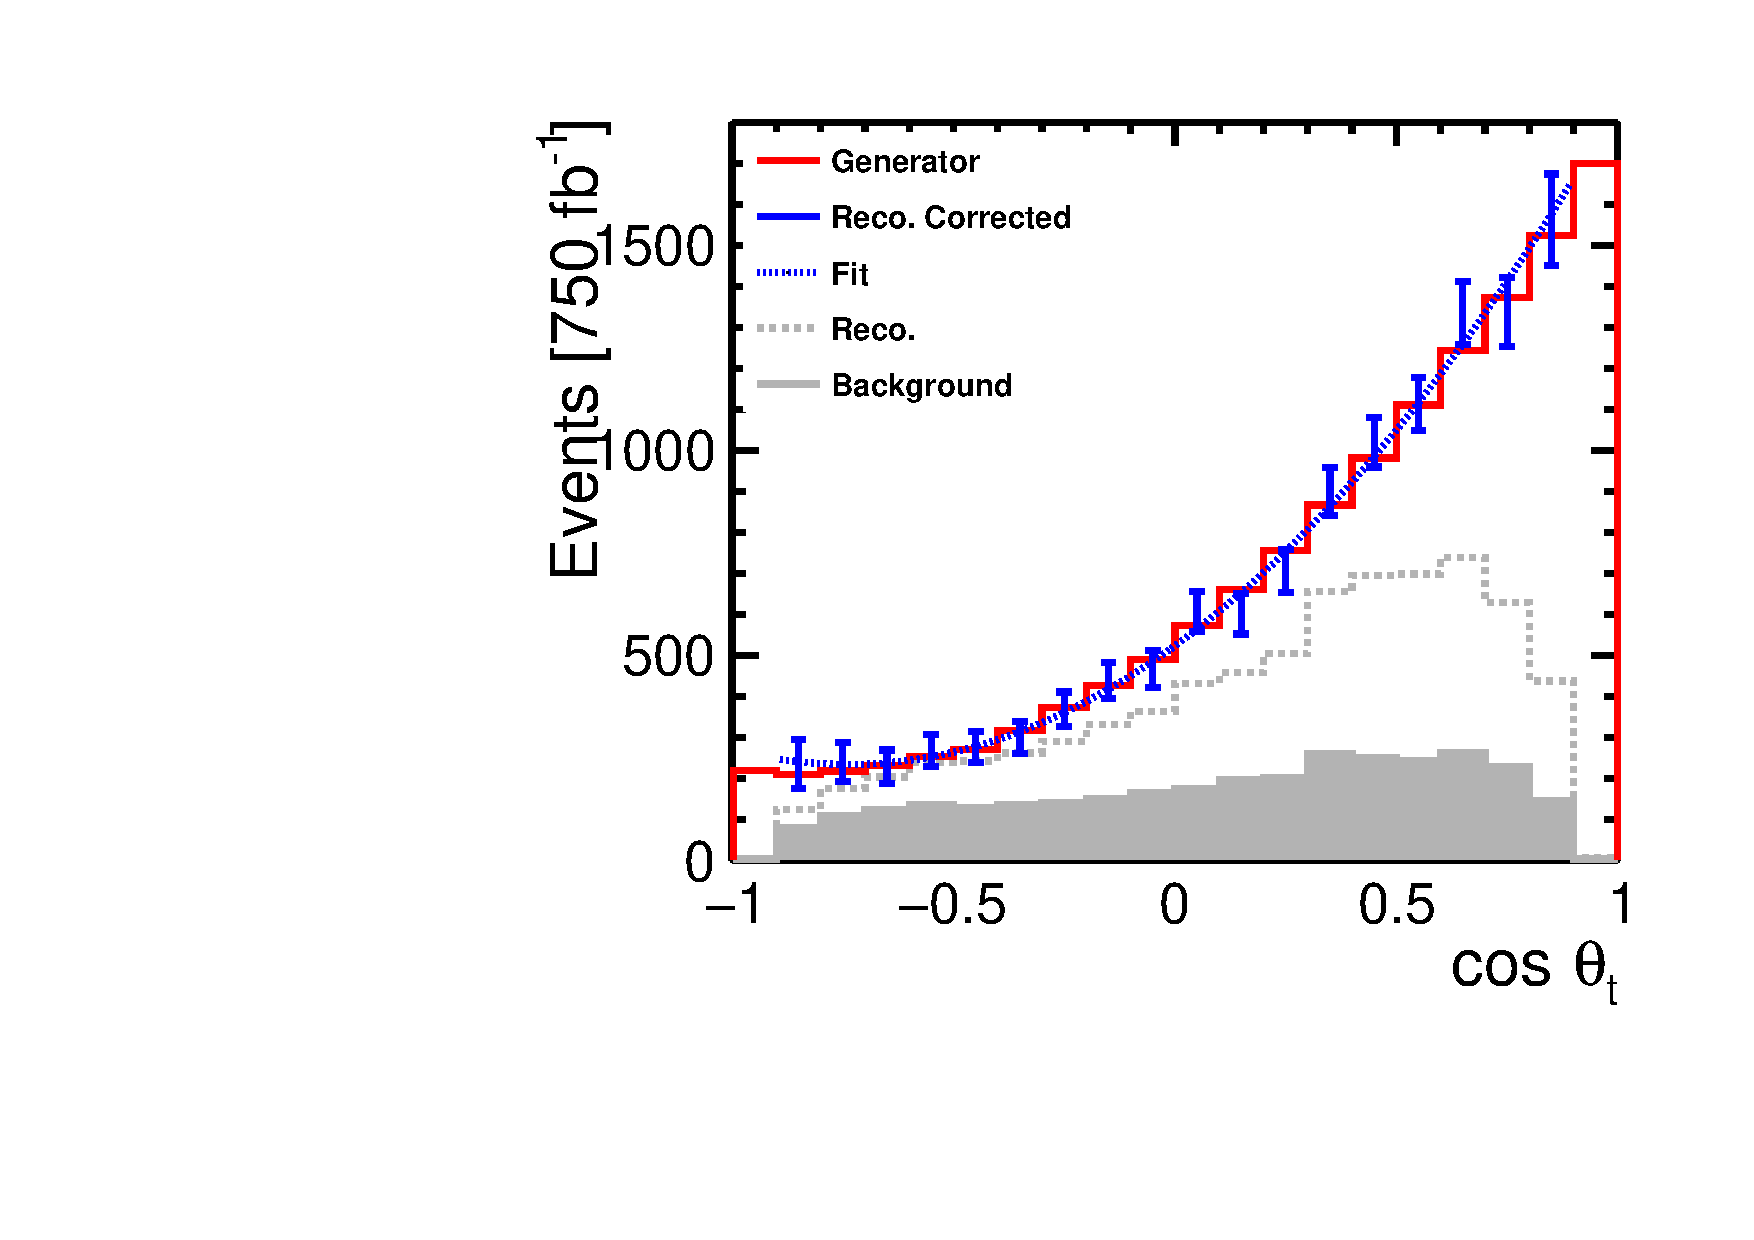
\includegraphics[width=0.99\linewidth]{TopAnalysis/figures/ThetaPlots_1200GeVNeg.pdf} 
    \caption{High energy, -80\% polarization} 
    \vspace{4ex}
  \end{subfigure}%% 
  \begin{subfigure}[]{0.5\linewidth}
    \centering
    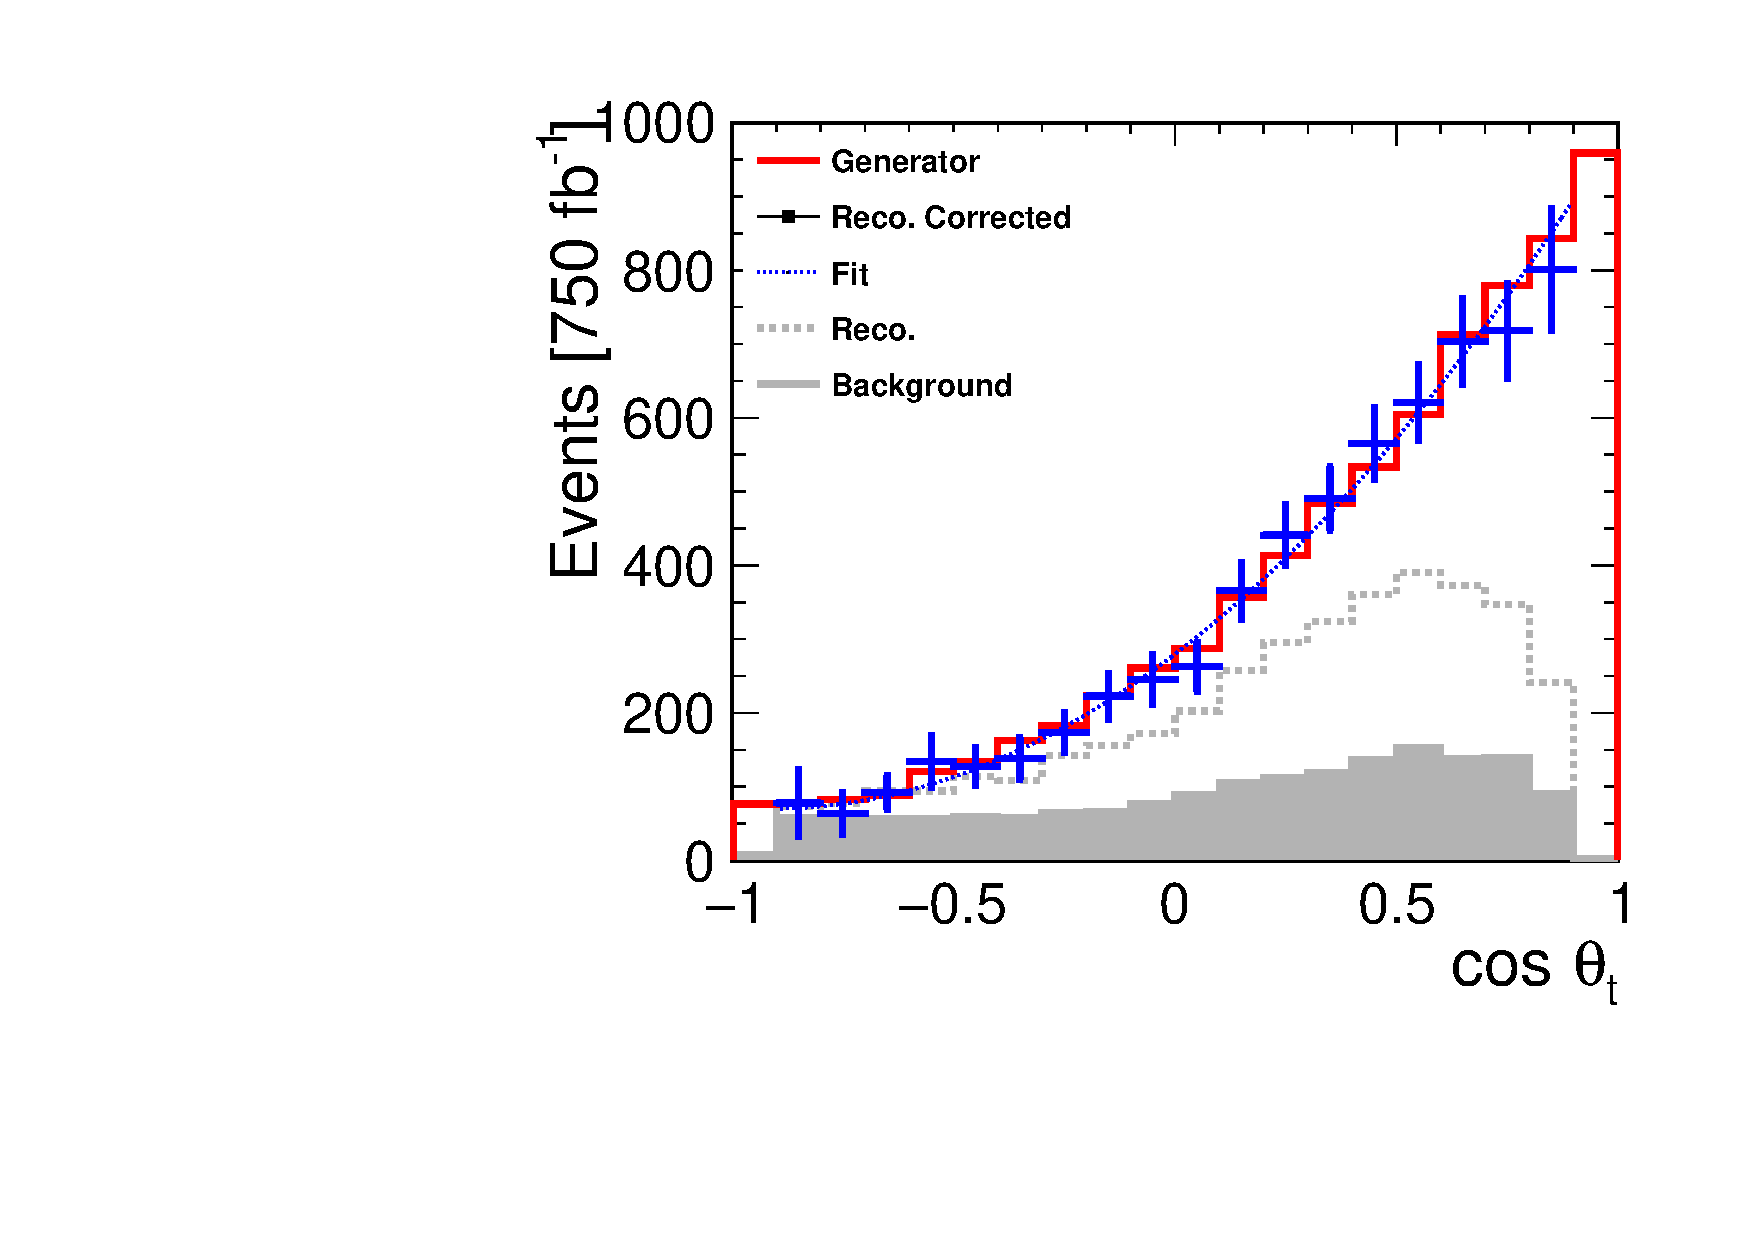
\includegraphics[width=0.99\linewidth]{TopAnalysis/figures/ThetaPlots_1200GeVPos.pdf} 
    \caption{High energy, +80\% polarization} 
    \vspace{4ex}
  \end{subfigure} 
  \begin{subfigure}[]{0.5\linewidth}
    \centering
    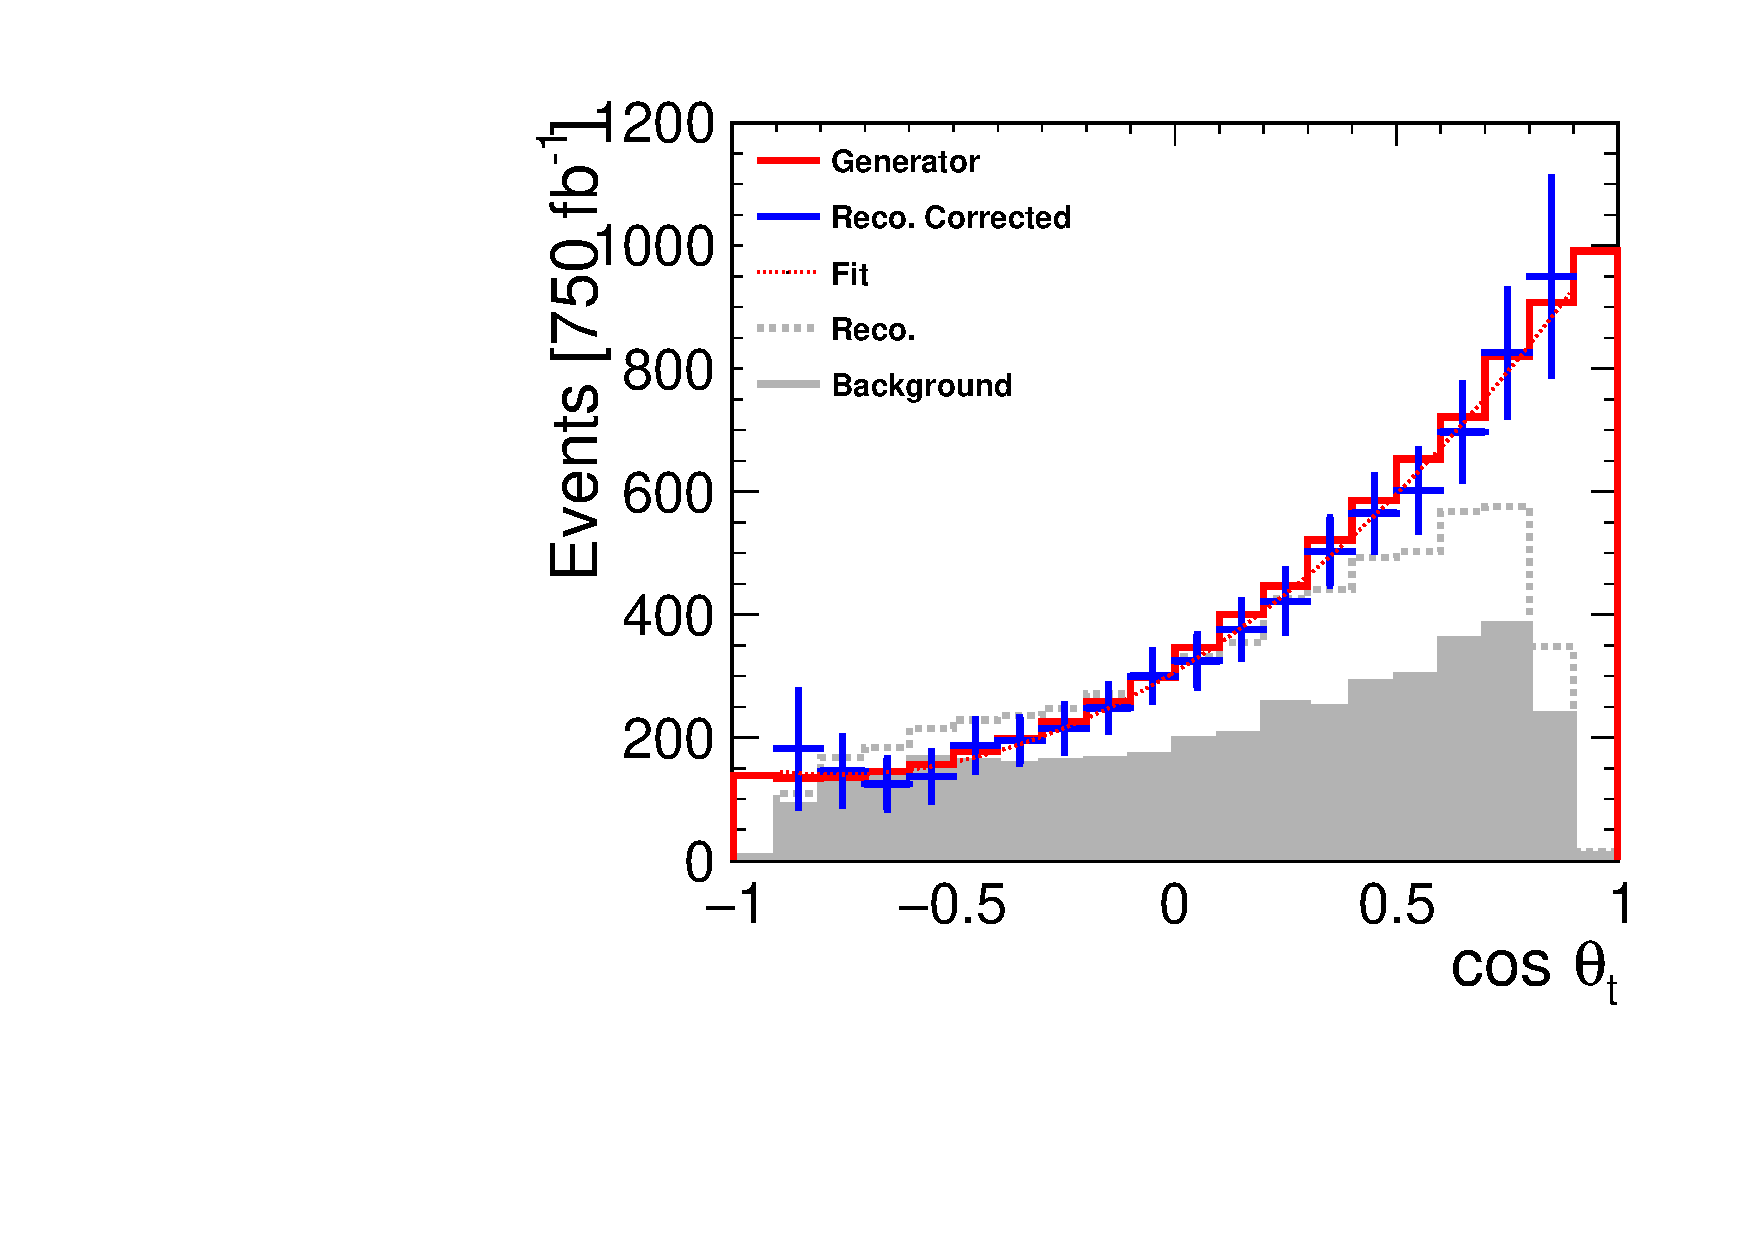
\includegraphics[width=0.99\linewidth]{TopAnalysis/figures/ThetaPlots_900GeVNeg.pdf} 
    \caption{Mid energy, -80\% polarization} 
    \vspace{4ex}
  \end{subfigure}%% 
  \begin{subfigure}[]{0.5\linewidth}
    \centering
    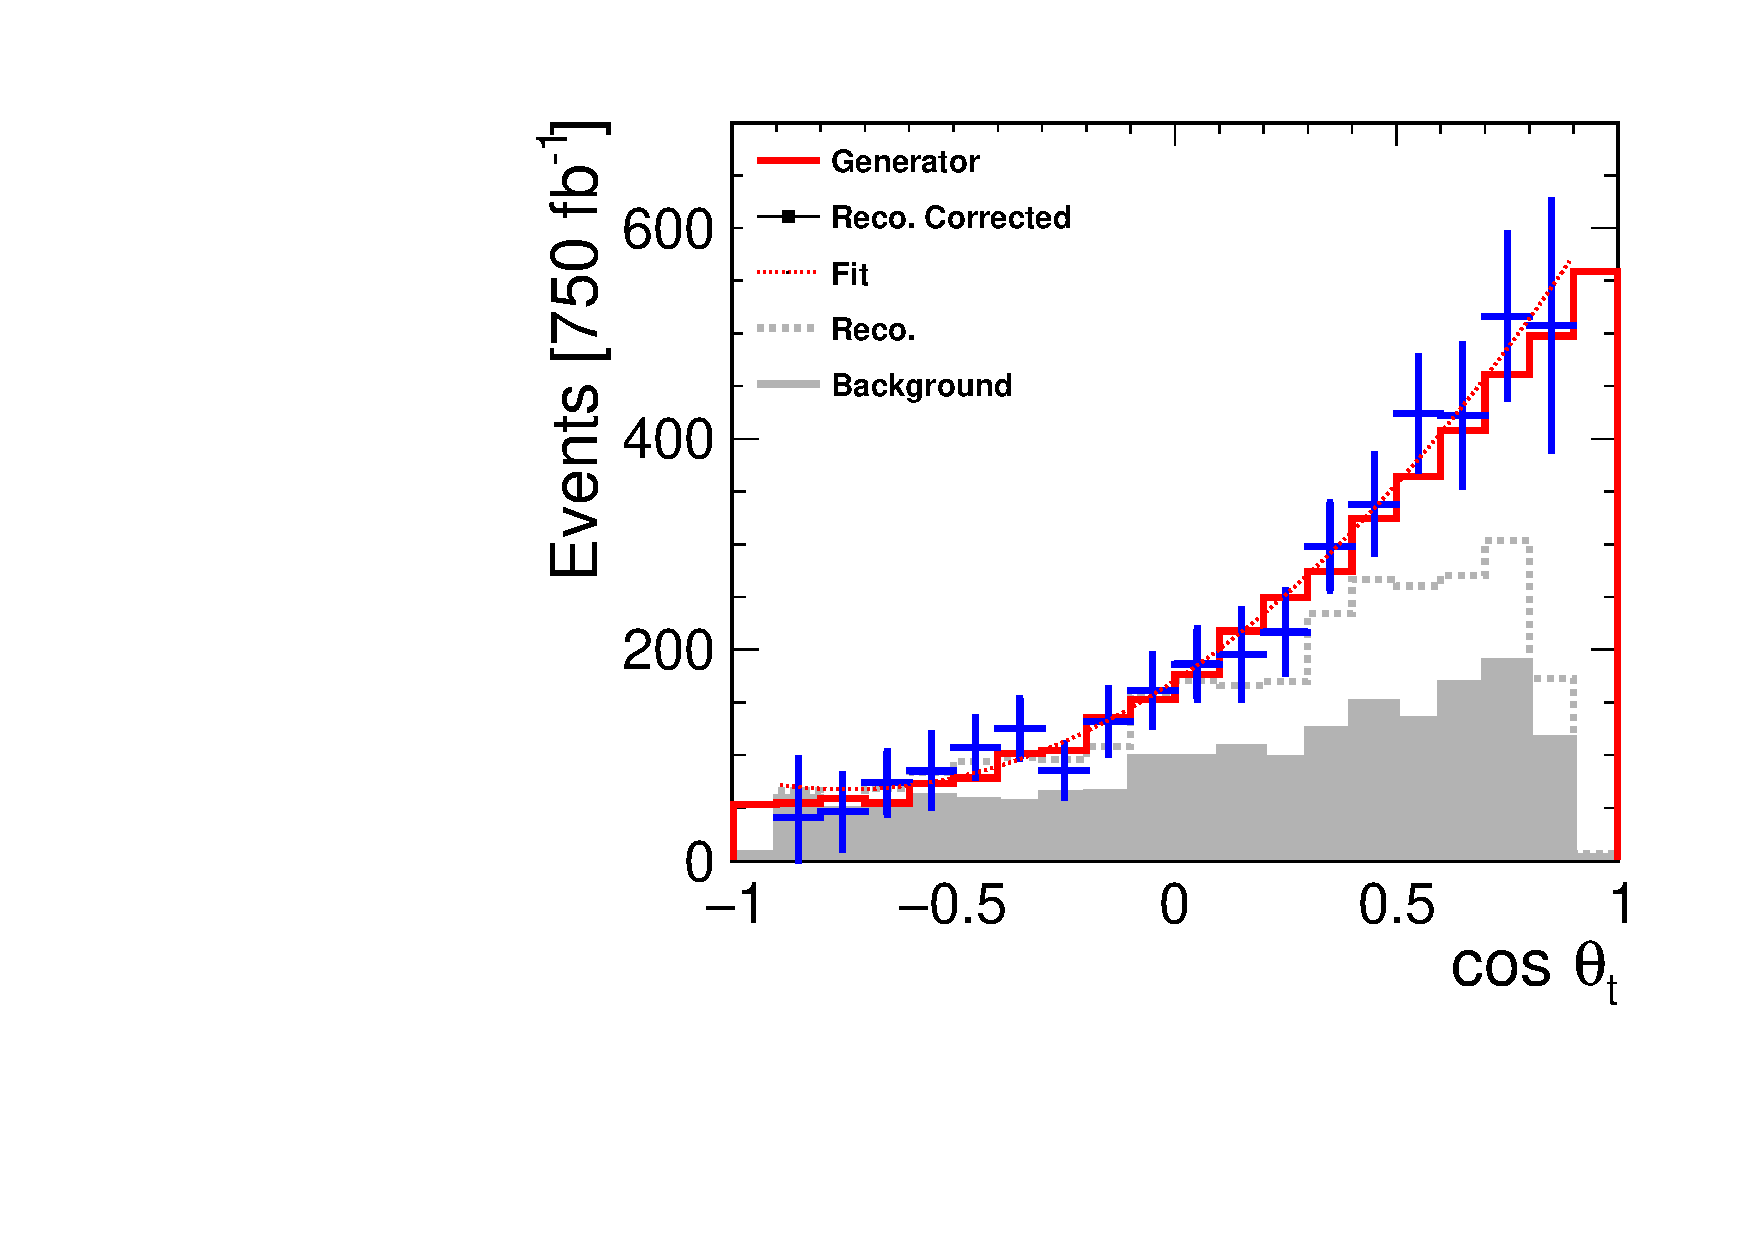
\includegraphics[width=0.99\linewidth]{TopAnalysis/figures/ThetaPlots_900GeVPos.pdf} 
    \caption{Mid energy, +80\% polarization} 
    \vspace{4ex}
  \end{subfigure}
  \begin{subfigure}[]{0.5\linewidth}
    \centering
    \includegraphics[width=0.99\linewidth]{TopAnalysis/figures/ThetaPlots_400GeVNeg.pdf} 
    \caption{Low energy, -80\% polarization} 
    \vspace{4ex}
  \end{subfigure}%% 
  \begin{subfigure}[]{0.5\linewidth}
    \centering
    \includegraphics[width=0.99\linewidth]{TopAnalysis/figures/ThetaPlots_400GeVPos.pdf} 
    \caption{Low energy, +80\% polarization} 
    \vspace{4ex}
  \end{subfigure}
  \caption[Final corrected angular distributions from which $A_{FB}^t$ and $\sigma_{Total}$ are extracted]{Angular distributions for all energy and polarization bins at generator, reconstructed and corrected levels along with the final fits from which $A_{FB}^t$ and $\sigma_{Total}$ are extracted. In all cases a luminosity of 750 fb$^{-1}$ is assumed for each beam polarization.}
  \label{fig:finalfits}
\end{figure}

\begin{table}
  \centering
  \begin{tabular}{l|c|c|c|c|c|c}
    \toprule
     Energy & $A_{FB}^t$ & $A_{FB}^t$  & $\Delta A^t_{FB}$ &  $\sigma$  &  $\sigma$  &  $\Delta\sigma$ \\
     (GeV) & (Gen.) & (Reco.) &  &  (Gen)(fb) &  (Reco)(fb) &  fb)\\
     \midrule
     \midrule
     \multicolumn{7}{l}{P(e$^-$)=-80\%} \\
     \midrule
     \midrule
    $>=$1200  & 0.563 & 0.563 & 0.018 & 18.4 & 18.4 & 0.37 \\
    \midrule
    900-1200  & 0.547 & 0.546 & 0.034 & 11.0 & 11.0 & 0.38 \\
    \midrule
    400-900   & 0.457 & 0.458 & 0.081 & 16.6 & 16.6 & 1.31 \\
    \midrule
    \midrule
   \multicolumn{7}{l}{ P(e$^-$)=+80\%}\\
    \midrule
    \midrule
    $>=$1200  & 0.621 & 0.621 & 0.024 & 9.8 & 9.8 & 0.28 \\
    \midrule
    900-1200  & 0.605 & 0.589 & 0.045 & 5.8 & 5.9 & 0.29 \\
    \midrule
    400-900   & 0.525 & 0.514 & 0.105 & 8.7 & 8.6 & 0.83 \\
    \bottomrule
  \end{tabular}
  \caption{Values and statistical uncertainties for $A_{FB}^t$ and cross section as extracted from performing a fit to $\cos\theta$ for each energy and polarization.}
  \label{tab:finalfitresults}
\end{table}

Overall it is seen that the typical uncertainties achieved are at the few per cent level. Already this is an order of magnitude better than the precision seen at the \ac{LHC}, $\mathcal{O}$(30\%)\cite{Bai:2011uk}, which is limited by the inability to distinguish tops produced via quark-quark interactions from those produced by gluon interactions. A factor of $\sim$$\sqrt{2}$ is seen between the equivalent results for each polarization, consistent with the factor of 2 difference in the $t\bar{t}$ cross section for each polarization. This indicates the reconstruction and event selection method is equally effective for both polarizations. The precision is seen to get worse for the lower energy bins. This is to be expected given that the reconstruction was designed with the focus of reconstructing events in which the top decay products are highly boosted. In the case of lower energy events the reconstruction is known to fail with neither fat jet corresponding to the complete decays products of the hadronic top. As a result these events typically fail the quality cuts leading to a low signal efficiency and so a large statistical uncertainty is introduced from  performing large efficiency corrections before the final fit.

It should be noted that these results are consistent with those seen for the alternative version of this analysis\cite{TopPaperDraft}. In that version of the analysis the lepton finding, top reconstruction, $\sqrt{s'}$ determination and event selection are all done in a completely different way to what is presented here, however the methods used for extracting the cross section and $A_{FB}^t$, and the treatment of uncertainties are identical for both analyses. The expected precision for the cross section and $A_{FB}^t$ in this alternative version of the analysis is entirely consistent in the precision obtained with that presented above as shown in \reftab{tab:RickardResults}. 

\begin{table}
  \centering
  \begin{tabular}{l|c|c|c|c|c|c}
    \toprule
    Energy & $A_{FB}^t$ & $A_{FB}^t$  & $\Delta A^t_{FB}$ &  $\sigma$  &  $\sigma$  &  $\Delta\sigma$ \\
    (GeV) & (Gen.) & (Reco.) &  &  (Gen)(fb) &  (Reco)(fb) &  fb)\\
    \midrule
    \midrule
    \multicolumn{7}{l}{P(e$^-$)=-80\%} \\
    \midrule
    \midrule
    $>=$1200  & 0.563 & 0.561 & 0.021 & 18.4 & 18.4 & 0.5 \\
    \midrule
    \midrule
    \multicolumn{7}{l}{ P(e$^-$)=+80\%}\\
    \midrule
    \midrule
    $>=$1200  & 0.621 & 0.618 & 0.023 & 9.8 & 9.9 & 0.31 \\
    \bottomrule
  \end{tabular}
  \caption{Values and statistical uncertainties for $A_{FB}^t$ and cross section as extracted from the alternative version of the analysis\cite{TopPaperDraft}.}
  \label{tab:RickardResults}
\end{table}

\section{Systematics}
\label{sec:topsystematics}

On top of the statistical uncertainty there are several additional sources of uncertainty that arise from systematic effects. A description of each effect considered is given below. 

\subsection{Background Normalization}

Following the event selection stage it was assumed that any remaining backgrounds could be removed without introducing an additional statistical uncertainty as this can be made arbitrarily small with a large enough sample size. While this is true, there will still be a theoretical uncertainty on the background cross sections which cannot be avoided. Here we assumed a conservative value of 5\% on the dominant backgrounds ($qqqql\nu, qql\nu l\nu,qq$.) While we assumed a lower value of 1\% during our treatment of the Higgs analysis, it was deemed necessary to increase this value here as for backgrounds such as $qq$ to resemble a six fermion final state requires the event to be in the tails of the kinematic distributions which are typically less well modelled. Assuming this value of 5\% for the theoretical uncertainty on each background, the analysis was repeated twice for each dominant background, once where the background is scaled to be 5\% greater than what is assumed in the subtraction step, once where it is 5\% lower. The presence of the excess background (\/deficit in signal events) will have a significant impact on the fit results, particularly in the cross section measurement. For each background the systematic uncertainty on the cross section and $A_{FB}^t$ was taken to be half the difference between the values observed for $\pm$5\%. The overall uncertainty from the background normalization was taken to be the sum in quadrature of all the individual background uncertainties. The results of this study are shown in \reftab{tab:bkgnorm}.

\begin{table}
  \centering
  \begin{tabular}{l|c|c|c|c|c|c}
    \toprule
     Energy & $A_{FB}^t$ & $\Delta A_{FB}^t$  & $\Delta A^t_{FB}$ &  $\sigma$  &  $\Delta\sigma$  &  $\Delta\sigma$ \\
     (GeV) &  & (Stat.) & (Syst.) &  (fb) &  (Stat.)(fb) &  (Syst.)(fb)\\
     \midrule
     \midrule
     \multicolumn{7}{l}{P(e$^-$)=-80\%} \\
     \midrule
     \midrule
    $>=$1200   & 0.563 & 0.018 & 0.003 & 18.4 & 0.37 & 0.27\\
    \midrule
    900-1200   & 0.546 & 0.034 & 0.006 & 11.0 & 0.38 & 0.28\\
    \midrule
    400-900    & 0.458 & 0.081 & 0.006 & 16.6 & 1.31 & 0.46\\
    \midrule
    \midrule
   \multicolumn{7}{l}{ P(e$^-$)=+80\%}\\
    \midrule
    \midrule
    $>=$1200  & 0.621 & 0.024 & 0.003 & 9.8 & 0.28 & 0.13 \\
    \midrule
    900-1200  & 0.589 & 0.045 & 0.003 & 5.9 & 0.29 & 0.13 \\
    \midrule
    400-900   & 0.514 & 0.105 & 0.002 & 8.6 & 0.83 & 0.17 \\
    \bottomrule
  \end{tabular}
  \caption{Systematic uncertainties for $A_{FB}^t$ and cross section arising from theoretical uncertainties on the background normalization.}
  \label{tab:bkgnorm}
\end{table}

One can see that the normalization uncertainty on $A_{FB}^t$ is relatively insignificant, however it is larger for the cross section as expected. In both cases the uncertainty is still dominated by the statistical component rather than the systematic.

\subsection{Background Shape}

As well as an uncertainty on the overall background normalization, there will also be a theoretical uncertainty on the shape of the background distribution. This is important to consider as $A_{FB}^t$ is entirely dependent on the shape of the $\cos\theta$ distribution. In order to quantify any effect this could have, a linear gradient was introduced in the total background distribution before the nominal background is subtracted from each bin. By a linear gradient it is meant that the $\cos\theta=1$ bin would be scaled by X\%, the $\cos\theta=-1$ bin by -X\% and all bins inbetween are scaled according to a linear distribution going from -X to X. A value of 2\% was chosen for the gradient. The result of applying this gradient is shown in \reftab{tab:bkggrad}.

\begin{table}
  \centering
  \begin{tabular}{l|c|c|c|c|c|c}
    \toprule
     Energy & $A_{FB}^t$ & $\Delta A_{FB}^t$  & $\Delta A^t_{FB}$ &  $\sigma$  &  $\Delta\sigma$  &  $\Delta\sigma$ \\
     (GeV) &  & (Stat.) & (Syst.) &  (fb) &  (Stat.)(fb) &  (Syst.)(fb)\\
     \midrule
     \midrule
     \multicolumn{7}{l}{P(e$^-$)=-80\%} \\
     \midrule
     \midrule
    $>=$1200   & 0.563 & 0.018 & 0.006 & 18.4 & 0.37 & 0.04\\
    \midrule
    900-1200   & 0.546 & 0.034 & 0.015 & 11.0 & 0.38 & 0.09\\
    \midrule
    400-900    & 0.458 & 0.081 & 0.013 & 16.6 & 1.31 & 0.08\\
    \midrule
    \midrule
   \multicolumn{7}{l}{ P(e$^-$)=+80\%}\\
    \midrule
    \midrule
    $>=$1200  & 0.621 & 0.024 & 0.006 & 9.8 & 0.28 & 0.03 \\
    \midrule
    900-1200  & 0.589 & 0.045 & 0.012 & 5.9 & 0.29 & 0.05 \\
    \midrule
    400-900   & 0.514 & 0.105 & 0.009 & 8.6 & 0.83 & 0.04 \\
    \bottomrule
  \end{tabular}
  \caption{Systematic uncertainties for $A_{FB}^t$ and cross section arising from theoretical uncertainties on the background shape.}
  \label{tab:bkggrad}
\end{table}

The uncertainty on the background shape causes a larger effect on $A_{FB}^t$ than on the cross section as expected. Ultimately the total uncertainty is still dominated by the statistical component. 

\subsection{Luminosity}

Is is anticipated that an uncertainty of 0.3\% can be achieved on the luminosity measurement at \ac{CLIC}. Incorrect measurement of the luminosity will directly affect the cross section measurement as $\sigma= \mathcal{L}/N$, however it also has an indirect effect from the fact the background subtraction will no longer be correct which can affect the $A_{FB}^t$ measurement. The effect of the luminosity uncertainty is shown in \reftab{tab:lumisys}. Ultimately this is seen to be small compared to the uncertainty from the background normalization or statistical component.

\begin{table}
  \centering
  \begin{tabular}{l|c|c|c|c|c|c}
    \toprule
     Energy & $A_{FB}^t$ & $\Delta A_{FB}^t$  & $\Delta A^t_{FB}$ &  $\sigma$  &  $\Delta\sigma$  &  $\Delta\sigma$ \\
     (GeV) &  & (Stat.) & (Syst.) &  (fb) &  (Stat.)(fb) &  (Syst.)(fb)\\
     \midrule
     \midrule
     \multicolumn{7}{l}{P(e$^-$)=-80\%} \\
     \midrule
     \midrule
    $>=$1200   & 0.563 & 0.018 & 0.001 & 18.4 & 0.37 & 0.10\\
    \midrule
    900-1200   & 0.546 & 0.034 & 0.001 & 11.0 & 0.38 & 0.10\\
    \midrule
    400-900    & 0.458 & 0.081 & 0.001 & 16.6 & 1.31 & 0.13\\
    \midrule
    \midrule
   \multicolumn{7}{l}{ P(e$^-$)=+80\%}\\
    \midrule
    \midrule
    $>=$1200  & 0.621 & 0.024 & 0.001 & 9.8 & 0.28 & 0.05 \\
    \midrule
    900-1200  & 0.589 & 0.045 & 0.001 & 5.9 & 0.29 & 0.05 \\
    \midrule
    400-900   & 0.514 & 0.105 & 0.001 & 8.6 & 0.83 & 0.06 \\
    \bottomrule
  \end{tabular}
  \caption{Systematic uncertainties for $A_{FB}^t$ and cross section arising from finite precision on integrated luminosity.}
  \label{tab:lumisys}
\end{table}


\subsection{Bias Towards Generator $A_{FB}^t$}

It is possible that in performing the bin by bin efficiency corrections to account for misreconstructed events a bias could have been introduced in the reconstructed $A_{FB}^t$. One way that this can be checked is by looking at the signal efficiency as a function of $\cos\theta$. If the efficiency corrections are only acting to correct for detector effects and not introducing a bias this distribution should be symmetric with a lower efficiency in the high $|\cos\theta|$ regions due to the detector acceptance. The signal efficiencies for each bin are shown in \reffigs{fig:sigefficienciesa} and \ref{fig:sigefficienciesb}. Note that without placing a cut on the lepton momentum in the lowest $\sqrt{s'}$ bin, an asymmetric efficiency distribution is observed. This is a result of the fact the efficiency for correctly identifying the lepton is worse for lower momentum leptons (see \refsec{sec:lepfinding}) and so the chance of the top charge tagging being incorrect increases in this region. When the top charge is misidentified, the reconstructed angle in the $t\bar{t}$ rest frame will be in the wrong hemisphere. Due to a non zero $A_{FB}^t$ there will be a net migration from the forward to backward regions. Thus when looking at the ratio of events in a bin to the number of events at generator level, the bins in the backward region will appear to have a higher efficiency than the forward region.

\begin{figure}
  \centering
  \begin{subfigure}{.5\textwidth}
    \centering
    \includegraphics[width=0.9\textwidth]{TopAnalysis/figures/efficiency_HighE.pdf}
    \caption{$>=$1200 GeV, -80\% polarization}
  \end{subfigure}%
  \begin{subfigure}{.5\textwidth}
    \centering
    \includegraphics[width=0.9\textwidth]{TopAnalysis/figures/efficiency_MidE.pdf}
    \caption{900-1200 GeV, -80\% polarization}
  \end{subfigure}
  \caption{Efficiency for reconstructing signal events in the correct $\cos\theta$ bins.}
  \label{fig:sigefficienciesa}
\end{figure}

\begin{figure}
  \centering
  \begin{subfigure}{.5\textwidth}
    \centering
    \includegraphics[width=0.9\textwidth]{TopAnalysis/figures/efficiency_LowE.pdf}
    \caption{400-900 GeV, -80\% polarization}
  \end{subfigure}%
  \begin{subfigure}{.5\textwidth}
    \centering
    \includegraphics[width=0.9\textwidth]{TopAnalysis/figures/efficiency_LowE_NoLepCut.pdf}
    \caption{400-900 GeV, -80\% polarization, no cut on lepton momentum}
  \end{subfigure}
  \caption{Efficiency for reconstructing signal events in the correct $\cos\theta$ bins.}
  \label{fig:sigefficienciesb}
\end{figure}

While the efficiencies do appear to be approximately symmetric, a more robust test can be performed by running the analysis on samples generated with a different $A_{FB}^t$ and seeing what $A_{FB}^t$ is obtained after reconstruction and event selection is performed. To avoid generating large new samples, samples with an alternative $A_{FB}^t$ were produced by sampling the full signal sample using \refeq{eq:afbfit} as the probability density function with the desired $A_{FB}^t$. In all cases the signal efficiency corrections applied are those calculated for the nominal $A_{FB}^t$. To measure the bias a linear fit of the generator $A_{FB}^t$ vs reconstructed $A_{FB}^t$ was performed. In the ideal case these two quantities should be directly proportional returning a gradient of one. The distribution of the reconstructed and generator $A_{FB}^t$ for each bin is shown in \reffig{fig:biassys}.

\begin{figure}
  \centering
  \begin{subfigure}{.6\textwidth}
    \centering
    \includegraphics[width=0.9\textwidth]{TopAnalysis/figures/BiasHighE.pdf}
    \caption{$>=$1200 GeV}
  \end{subfigure}
  \begin{subfigure}{.6\textwidth}
    \centering
    \includegraphics[width=0.9\textwidth]{TopAnalysis/figures/BiasMidE.pdf}
    \caption{900-1200 GeV}
  \end{subfigure}
  \begin{subfigure}{.6\textwidth}
    \centering
    \includegraphics[width=0.9\textwidth]{TopAnalysis/figures/BiasLowE.pdf}
    \caption{400-1200 GeV}
  \end{subfigure}
  \caption{Correlation between the reconstructed and generator $A_{FB}^t$ for each $\sqrt{s'}$ bin, -80\% polarization.}
  \label{fig:biassys}
\end{figure}

In all cases a slight bias is seen with the high, middle and low energy fits yielding gradients of 0.92$\pm$0.02, 0.93$\pm$0.04 and 0.83$\pm$0.05 respectively. The fact the bias is largest in the lowest $\sqrt{s'}$ bin is to be expected as the efficiency corrections are largest in this bin. In all cases the fit reveals a bias towards the original generator values, with an $A_{FB}^t$ greater than this being underestimated and vice versa. While this is not the ideal case, it should be noted that the relationship between the reconstructed and generator level $A_{FB}^t$ is still linear and as such a simple mapping between the two can be applied to recover the generator level value. The fractional uncertainty introduced on $A_{FB}^t$ from this additional correction corresponds to the fractional uncertainty on the gradient of the fits in \reffig{fig:biassys}. It is further worth noting that the uncertainty on this fit has no dependence on measured values as the fit uses only simulated data. As such the uncertainties can in principle be made arbitrarily small with a large enough statistical sample. For now, the uncertainty is conservatively taken to be that seen for the current sample size for -80\% polarization. For the +80\% polarization the current sample sizes are significantly smaller and so would yield much higher uncertainties. As a result, it is assumed that the same fractional uncertainty on $A_{FB}^t$ as seen for the -80\% polarization could be achieved for the +80\% polarization in future. The resulting uncertainty introduced on $A_{FB}^t$ for each polarization is shown in \reftab{tab:biassys}.

\begin{table}
  \centering
  \begin{tabular}{l|c|c|c}
    \toprule
    Energy (GeV)& $A_{FB}^t$ & $\Delta A_{FB}^t$  (Stat.) & $\Delta A^t_{FB}$ (Syst.)  \\
    \midrule
    \midrule
    \multicolumn{4}{l}{P(e$^-$)=-80\%} \\
    \midrule
    \midrule
    $>=$1200   & 0.563 & 0.018 & 0.014\\
    \midrule
    900-1200   & 0.546 & 0.034 & 0.023\\
    \midrule
    400-900    & 0.458 & 0.081 & 0.029\\
    \midrule
    \midrule
    \multicolumn{4}{l}{ P(e$^-$)=+80\%}\\
    \midrule
    \midrule
    $>=$1200  & 0.621 & 0.024 & 0.015\\
    \midrule
    900-1200  & 0.589 & 0.045 & 0.024\\
    \midrule
    400-900   & 0.514 & 0.105 & 0.032\\
    \bottomrule
  \end{tabular}
  \caption{Systematic uncertainties accounting for bias in $A_{FB}^t$ from signal efficiency corrections.}
  \label{tab:biassys}
\end{table}

The systematic effect of the bias is seen to produce the largest systematic uncertainty on $A_{FB}^t$, however it is still less than the statistical component.

\subsection{Unquantified Effects}

As well as the effects above which have been found to have significant contributions to the overall uncertainty on the measurements, several other effects have been examined but found to have negligible impacts on the final measurements and as such are not quantified here. There are three main effects of this type:

The first of these was the effect of the fit range. This was assessed by simply varying the range of $\mid\cos\theta\mid$ over which the fit is performed from 0.7 to 1.0 in 0.1 intervals. This was shown to change the statistical precision on the final result but not the central values for $A_{FB}^t$ or the cross section. This is somewhat to be expected as the distribution still has the correct shape in the central region and so the fit should still extract the same values as are seen at generator level.

The second effect was from changing the values used for the \ac{BDT} cut. Again this was found to only effect the uncertainty on the final results but not the central value as it only changes the signal to background ratio, but as the background is subtracted anyway this has no effect on the final distribution, only on the statistical uncertainty of each bin.

The final effect was considered was the relative performance of the electron and muon signal channels. While this is not something that should change the final results, a large difference between the two channels could indicate an area for improvement in future. The performance of each channel was evaluated by excluding the other lepton channel from the analysis entirely and then looking at how the final fit results and their uncertainties changed, accounting for the slightly different cross sections for each channel. Ultimately it was found that the central values of the fits were in agreement but that the electron channel had a slightly larger uncertainty. This arises from the arguments already described in \refsec{sec:lepfinding}, which state that because the electron reconstruction only relies on two detector components (the tracker and \ac{ECAL}) it has a higher chance of being missed or wrongly identified as a photon compared to the muon which penetrates the full detector. Events in which the electron is not correctly reconstructed will typically be removed by the quality cuts of the analysis leading to a reduced signal efficiency. Thankfully however, due to the fact the lepton finding presented here is based on the Pandora \ac{PID} of the particles, due to the ongoing efforts to improve Pandora it is likely that the efficiency in this channel will improve by the time the measurement can be performed. 

As well as these effects for which no additional systematic uncertainty is assigned as they are found to be negligible, there is one unquantified effect that should be taken into account when performing the measurement. As already mentioned, the centrally produced \ac{CLIC} samples currently only use one event generator and hadronization handler (WHIZARD and PYTHIA). Ideally one would try several different Monte Carlo models for the analysis to see if there is a systematic effect from the modeling. This is particularly true here where the jet substructure variables used for event selection could be particularly sensitive to the hadronization modeling. Efforts have been made to remain as insensitive to the modeling as possible (such as using ``microjets'' rather than PFOs for calculating these variables), however the sensitivity is something that should be quantified in future.

\subsection{Summary}
\begin{table}
  \centering
  \begin{tabular}{l|c|c|c|c|c|c|c}
    \toprule
    \midrule
    \multicolumn{8}{l}{P(e$^-$)=-80\%} \\
    \midrule
    \midrule
   Energy &  &  &     \multicolumn{5}{c}{Systematic Effects} \\
    (GeV) & $A_{FB}^t$ & Stat. & Total & Bias & Lumi. & Bkg Norm & Bkg Shape\\
    \midrule
    $>=$1200   & 0.563 & 0.018 & 0.015 & 0.014 & 0.001 & 0.003 & 0.006\\
    \midrule
    900-1200   & 0.546 & 0.034 & 0.028 & 0.023 & 0.001 & 0.006 & 0.015\\
    \midrule
    400-900    & 0.458 & 0.081 & 0.032 & 0.029 & 0.001 & 0.006 & 0.013\\
    \midrule
    \midrule
    Energy &  &   &     \multicolumn{5}{c}{Systematic Effects} \\
    (GeV) & $\sigma$ (fb) & Stat. & Total & Bias & Lumi. & Bkg Norm & Bkg Shape\\
    \midrule
    $>=$1200   & 18.41 & 0.37 & 0.29 & -- & 0.10 & 0.27 & 0.04\\
    \midrule
    900-1200   & 11.01 & 0.38 & 0.31 & -- & 0.10 & 0.28 & 0.10\\
    \midrule
    400-900    & 16.56 & 1.31 & 0.48 & -- & 0.13 & 0.46 & 0.08\\
    \midrule
    \multicolumn{8}{c}{}\\
    \midrule
    \midrule
    \multicolumn{8}{l}{ P(e$^-$)=+80\%}\\
    \midrule
    \midrule
   Energy &  &   &     \multicolumn{5}{c}{Systematic} \\
    (GeV) & $A_{FB}^t$ & Stat. & Total & Bias & Lumi. & Bkg Norm & Bkg Shape\\
    \midrule
    $>=$1200   & 0.621 & 0.024 & 0.016 & 0.015 & 0.001 & 0.003 & 0.006\\
    \midrule
    900-1200   & 0.588 & 0.045 & 0.027 & 0.024 & 0.001 & 0.003 & 0.012\\
    \midrule
    400-900    & 0.514 & 0.105 & 0.034 & 0.032 & 0.001 & 0.002 & 0.010\\
    \midrule
    \midrule
    Energy &  &   &     \multicolumn{5}{c}{Systematic} \\
    (GeV) & $\sigma$ (fb) & Stat. & Total & Bias & Lumi. & Bkg Norm & Bkg Shape\\
    \midrule
    $>=$1200   & 9.84 & 0.28 & 0.14 & -- & 0.05 & 0.13 & 0.03\\
    \midrule
    900-1200   & 5.87 & 0.29 & 0.14 & -- & 0.05 & 0.13 & 0.05\\
    \midrule
    400-900    & 8.63 & 0.83 & 0.19 & -- & 0.06 & 0.17 & 0.04\\
    \bottomrule
  \end{tabular}
  \caption{Summary of statistical and systematic uncertainties for both polarizations and all energy ranges.}
  \label{finaltable}
\end{table}

The culmination of all the sources of uncertainty examined in the analysis is shown in \reftab{finaltable}. One can see that the uncertainty on all quantities is ultimately dominated by the statistical uncertainty. It is possible that several of the systematic uncertainties could be reduced in future, particularly the signal efficiency bias that is dependent on the number of events generated. As such the values given here are likely to represent a conservative estimate of the systematic uncertainty.


\section{Improvements}

While the work here is considered complete, there are still potential improvements that could be made between now and the time at which the measurement would be performed. The most minor of these would be to optimize the quality cuts used for each energy bin. This might yield a slight improvement in the statistical precision for the lowest energy bins as this could improve the signal efficiency, however as the low signal efficiency is largely a result of the failed reconstruction of the top in this region, the improvement is unlikely to be large. A larger improvement could be achieved by changing how the reconstruction of the tops is performed in this region. Because the decay products of the tops will be less collimated in this region, it may be possible to resolve all four quark jets within the event allowing a more reliable reconstruction of the top that is less sensitive to overlapping fat jets. In practice this would likely warrant a dedicated study, separate to the higher $\sqrt{s'}$ analysis.

As already mentioned, one significant missing component from the study at the minute is an understanding of the systematic uncertainty associated with the hadronization modeling. While it is not currently possible to study this within the current ILCSoft framework, this is certainly something that will be investigated in future before the measurement is performed. On a related note of improving ILCSoft, further improvements could be made with the development of a tau finder package. Currently the signal channel only consists of states where the leptonic top produces an electron or muon. If taus could be reliably found, the signal cross section could optimistically be increased by a factor of $\sim$50\% by including the tau channel. This would also mean a reduction in the background as the tau channel would no longer be included. 

A final potential improvement that has yet to be mentioned is the optimization of the luminosity split between each polarization. Currently it is assumed that the same integrated luminosity will be accrued for each beam polarization, however as can be seen in the current results, due to the lower cross section of the signal channel in the +80\% polarization configuration, the expected statistical precision for the variables measured for this polarization is worse. In order to perform a full optimization of the luminosity division it would be necessary to look both at the end effect on the precision of the electroweak form factors of the ttX vertex as well the effect on the wider \ac{CLIC} physics programme. As such it is not clear what the optimal division should be, however it is likely that an even split between both run configurations is not optimal.

\section{Conclusions}
\begin{table}[t]
  \centering
  \begin{tabular}{l|c|c}
    \toprule
    Energy (GeV) & $A_{FB}^t$ $\pm$ Stat. $\oplus$ Syst. & $\sigma$  $\pm$ Stat. $\oplus$ Syst.   \\
    \midrule
    \midrule
    \multicolumn{3}{l}{ P(e$^-$)=-80\%}\\
    \midrule
    $>=$1200   & 0.563 $\pm$ 0.018 $\oplus$ 0.015 & 18.41 $\pm$ 0.37 $\oplus$ 0.29\\
    \midrule
    900-1200   & 0.546 $\pm$ 0.034 $\oplus$ 0.028 & 11.01 $\pm$ 0.38 $\oplus$ 0.31\\
    \midrule
    400-900    & 0.458 $\pm$ 0.081 $\oplus$ 0.032 & 16.56 $\pm$ 1.31 $\oplus$ 0.48\\
    \midrule
    \midrule
    \multicolumn{3}{l}{ P(e$^-$)=+80\%}\\
    \midrule
    $>=$1200  & 0.621 $\pm$ 0.024 $\oplus$ 0.016 & 9.84 $\pm$ 0.28 $\oplus$ 0.14\\
    \midrule
    900-1200  & 0.588 $\pm$ 0.045 $\oplus$ 0.027 & 5.87 $\pm$ 0.29 $\oplus$ 0.14\\
    \midrule
    400-900   & 0.514 $\pm$ 0.105 $\oplus$ 0.034 & 8.63 $\pm$ 0.83 $\oplus$ 0.19\\
    \bottomrule
  \end{tabular}
  \caption{Final summary of the expected precisions attainable from the $t\bar{t}$ analysis.}
  \label{tab:conclusionnumbers}
\end{table}

In summary, we have presented an analysis looking at the measurement of the top forward backward asymmetry and $t\bar{t}$ cross section with the aim of probing the electroweak form factors of the ttX vertex. To maximize the available information the analysis was split into six bins corresponding to three different energy ranges and two different beam polarizations. Events were reconstructed using large radius fat jets to account for the highly collimated nature of the top decay products, and the substructure of these fat jets was used to perform event selection. The event selection was performed in two main sections. Initially cuts were applied to remove easily identifiable backgrounds and events in which the reconstruction has failed. Following this a pair of \ac{BDT}s were used to remove remaining background events with one \ac{BDT} trained to select high energy events and the other trained on low energy events. The selection was found to give high efficiencies for high energy bins and significantly lower efficiencies for lower energy bins due to poor jet reconstruction at this scale. The cross section and $A_{FB}^t$ are extracted using a second order fit to the production angle of the top following the subtraction of any remaining backgrounds and correction for finite signal efficiency. The results of applying this method are summarized in \reftab{tab:conclusionnumbers}. A detailed study of various systematic effects revealed that in all cases the uncertainty is dominated by the statistical component with the dominant systematic contributions for the cross section and $A_{FB}^t$ coming from the background normalization and bias introduced during efficiency corrections respectively. The final precision was found to be an order of magnitude better than what is seen at the \ac{LHC}\cite{Bai:2011uk} and is consistent with results obtained for an alternative version of the analysis\cite{TopPaperDraft}.

